\documentclass[twocolumn,secnumarabic,amssymb, nobibnotes, aps, prl,
superscriptaddress, nobalancelastpage]{revtex4}
\newcommand{\revtex}{REV\TeX\ }
\newcommand{\classoption}[1]{\texttt{#1}}
\newcommand{\macro}[1]{\texttt{\textbackslash#1}}
\newcommand{\m}[1]{\macro{#1}} \newcommand{\env}[1]{\texttt{#1}}
\setlength{\textheight}{9.5in} \usepackage{graphicx}
\setlength{\belowcaptionskip}{6pt}
\usepackage{amsmath} \usepackage{braket} \usepackage{epsfig}
\usepackage{upgreek}
\usepackage{textcomp}
\usepackage[free-standing-units]{siunitx}
\usepackage{xcolor}

\newcolumntype{N}{>{\centering\arraybackslash}m{1.3in}}
\newcolumntype{M}{>{\centering\arraybackslash}m{1.0in}}
\newcolumntype{G}{>{\centering\arraybackslash}m{0.5in}}
\newcolumntype{R}{>{\raggedleft\arraybackslash}m{0.4in}}

\newcommand{\tot}{\ensuremath{\sigma_{tot}}}
\newcommand{\totRD}{\ensuremath{\sigma_{A,A'}}(E)}
\newcommand{\rxn}{\ensuremath{\sigma_{rxn}}}
\newcommand{\el}{\ensuremath{\frac{\lowercase{d}\sigma}{\lowercase{d}\Omega}}}

\newcommand{\oSix}{\ensuremath{^{16}}O}
\newcommand{\oSeven}{\ensuremath{^{17}}O}
\newcommand{\oEight}{\ensuremath{^{18}}O}
\newcommand{\oSixEight}{\ensuremath{^{16,18}}O}

\newcommand{\neEight}{\ensuremath{^{18}}N\lowercase{e}}

\newcommand{\caForty}{\ensuremath{^{40}}C\lowercase{a}}
\newcommand{\caEight}{\ensuremath{^{48}}C\lowercase{a}}
\newcommand{\caAughtEight}{\ensuremath{^{40,48}}C\lowercase{a}}

\newcommand{\niSix}{\ensuremath{^{56}}N\lowercase{i}}
\newcommand{\niEight}{\ensuremath{^{58}}N\lowercase{i}}
\newcommand{\niSixty}{\ensuremath{^{60}}N\lowercase{i}}
\newcommand{\niOne}{\ensuremath{^{61}}N\lowercase{i}}
\newcommand{\niTwo}{\ensuremath{^{62}}N\lowercase{i}}
\newcommand{\niFour}{\ensuremath{^{64}}N\lowercase{i}}
\newcommand{\niEightFour}{\ensuremath{^{58,64}}N\lowercase{i}}
\newcommand{\niNat}{\ensuremath{^{\text{nat}}}N\lowercase{i}}

\newcommand{\rhThree}{\ensuremath{^{103}}R\lowercase{h}}

\newcommand{\snTwelve}{\ensuremath{^{112}}S\lowercase{n}}
\newcommand{\snFourteen}{\ensuremath{^{114}}S\lowercase{n}}
\newcommand{\snFifteen}{\ensuremath{^{115}}S\lowercase{n}}
\newcommand{\snSixteen}{\ensuremath{^{116}}S\lowercase{n}}
\newcommand{\snSeventeen}{\ensuremath{^{117}}S\lowercase{n}}
\newcommand{\snEighteen}{\ensuremath{^{118}}S\lowercase{n}}
\newcommand{\snNineteen}{\ensuremath{^{119}}S\lowercase{n}}
\newcommand{\snTwenty}{\ensuremath{^{120}}S\lowercase{n}}
\newcommand{\snTwo}{\ensuremath{^{122}}S\lowercase{n}}
\newcommand{\snFour}{\ensuremath{^{124}}S\lowercase{n}}
\newcommand{\snTwelveFour}{\ensuremath{^{112,124}}S\lowercase{n}}
\newcommand{\snNat}{\ensuremath{^{\text{\lowercase{nat}}}}S\lowercase{n}}
\newcommand{\snTwelveNatFour}{\ensuremath{^{112,\text{nat},124}}S\lowercase{n}}

\newcommand{\pbEight}{\ensuremath{^{208}}P\lowercase{b}}
\newcommand{\pbNat}{\ensuremath{^{\text{\lowercase{nat}}}}P\lowercase{b}}

% shell labels
\newcommand{\sOne}{s\ensuremath{_{\frac{1}{2}}}}
\newcommand{\pThree}{p\ensuremath{_{\frac{3}{2}}}}
\newcommand{\pOne}{p\ensuremath{_{\frac{1}{2}}}}
\newcommand{\dFive}{d\ensuremath{_{\frac{5}{2}}}}
\newcommand{\dThree}{d\ensuremath{_{\frac{3}{2}}}}
\newcommand{\fSeven}{f\ensuremath{_{\frac{7}{2}}}}
\newcommand{\fFive}{f\ensuremath{_{\frac{5}{2}}}}
\newcommand{\gNine}{g\ensuremath{_{\frac{9}{2}}}}
\newcommand{\gSeven}{g\ensuremath{_{\frac{7}{2}}}}
\newcommand{\hEleven}{h\ensuremath{_{\frac{11}{2}}}}

\newcommand{\tZero}{T\ensuremath{_{0}}}



\begin{document}

\begin{abstract}
    The neutron total cross sections \tot\ of $^{16,18}$O,
    $^{58,nat,64}$Ni, $^{103}$Rh, and $^{112,nat,124}$Sn have been measured at the Los Alamos
    Neutron Science Center (LANSCE) at intermediate energies (3 $\leq E_{n}
    \leq$ 450 MeV) by
    leveraging waveform digitizer technology. The results are in good agreement
    with previous measurements that used analog techniques,
    excepting small deviations at high energies. These data
    continue the campaign of
    \tot\ measurements we initiated with the case study of $^{40,48}$Ca in 2009.
    The \tot\ relative differences between isotopes are presented,
    revealing additional information about
    the isovector components needed for an accurate optical model (OM)
    description away from stability. Digitizer-enabled \tot-measurement
    techniques are discussed and a series of Dispersive Optical Model (DOM)
    analyses using these new data is presented, validating the DOM for modeling light
    systems (\oSixEight) and systems with open neutron shells (\niEightFour\ and \snTwelveFour).
\end{abstract}

\title{Isotopically-Resolved Neutron Total Cross Sections At
Intermediate Energies}

\author{C.~D.~Pruitt}  \email[Corresponding author:]{cdpruitt@wustl.edu}
\author{R.~J.~Charity}
\affiliation{Department of Chemistry, Washington University, St. Louis, MO 63130}
\author{L.~G.~Sobotka}
\affiliation{Department of  Chemistry, Washington University, St. Louis, MO 63130, USA}
\affiliation{Department of  Physics, Washington University, St. Louis, MO 63130, USA}
\author{D. E.~M.~Hoff}  
\affiliation{Department of Chemistry, Washington University, St. Louis, MO 63130}
\altaffiliation{Present Address: \textit{Department of Physics, University of
        Massachusetts-Lowell and
Astronomy, Michigan State University, East Lansing, MI 48824, USA}}

\author{K.~W.~Brown} \altaffiliation{Present Address: \textit{National
        Superconducting Cyclotron Laboratory, Departments of Physics and
Astronomy, Michigan State University, East Lansing, MI 48824, USA}}
\author{J.~M.~Elson}
\affiliation{Department of Chemistry, Washington University, St. Louis, MO 63130}

\author{M.C.~Atkinson}
\author{W.H.~Dickhoff}
\affiliation{Department of Physics, Washington University, St. Louis, MO 63130}

\author{H. Y. Lee}
\author{M. Devlin}
\author{N. Fotiadis}
\author{S. Mosby}
\affiliation{Los Alamos National Lab, Los Alamos, NM 87545, USA}
\maketitle

Neutron scattering is a direct, Coulomb-insensitive tool for probing the nuclear
environment. The simplest neutron-nucleus interaction quantity is 
the neutron total cross section, \tot, which provides fundamental information about
nuclear size and the ratio of elastic-to-inelastic components of nucleon 
scattering. Additionally, \tot\ data are thought to be tightly correlated with
a variety of structural nuclear properties of great interest
including the neutron skin of neutron-rich nuclei
\cite{Mahzoon2017} and thus the density dependence of the symmetry energy $L$,
an essential equation-of-state (EOS) input for neutron star
structure calculations \cite{Fattoyev2012, Vinas2014, Brown2000}.

In the crudest approximation, the ``strongly-absorbing sphere'' picture
explains the dependence of \tot\ on the size of the target nucleus and on the
energy of the incident neutron as a consequence of simple size-scaling:
\begin{equation} \label{SASAbsolute}
    \sigma_{tot}(E) = 2\pi(R + \lambdabar)^{2},
\end{equation}
where $R=r_{0}A^{\frac{1}{3}}$ and $\lambdabar$ is the reduced wavelength
of the incident neutron with energy $E$ in the center of mass \cite{Fernbach1949, Satchler1980}. 
%To compare \tot\ for two different targets of masses A and A$'$, the relative
%difference \totRD\ is useful:
%\begin{equation} \label{SASRelDiff}
%    \begin{split}
%        \totRD\ & \equiv
%    \frac{\sigma_{A}-\sigma_{A'}}{\sigma_{A}+\sigma_{A'}} \\
%    & =
%    \frac{r_{0}^{2}(A^{\frac{2}{3}}-A'^{\frac{2}{3}}) +
%    2\lambdabar r_{0}(A^{\frac{1}{3}}-A'^{\frac{1}{3}})}
%    {r_{0}^{2}(A^{\frac{2}{3}}+A'^{\frac{2}{3}}) +
%    2\lambdabar r_{0}(A^{\frac{1}{3}}+A'^{\frac{1}{3}}) + 2\lambdabar^{2}},
%    \end{split}
%\end{equation}
While on \textit{average}, experimental \tot\ data comport with this naive
model, the most prominent feature of experimental \tot\ data is the oscillatory
behavior centered about the average of Eq. \ref{SASAbsolute}, visible in Fig.
\ref{SASphereVsExperiment}.

\begin{figure}
    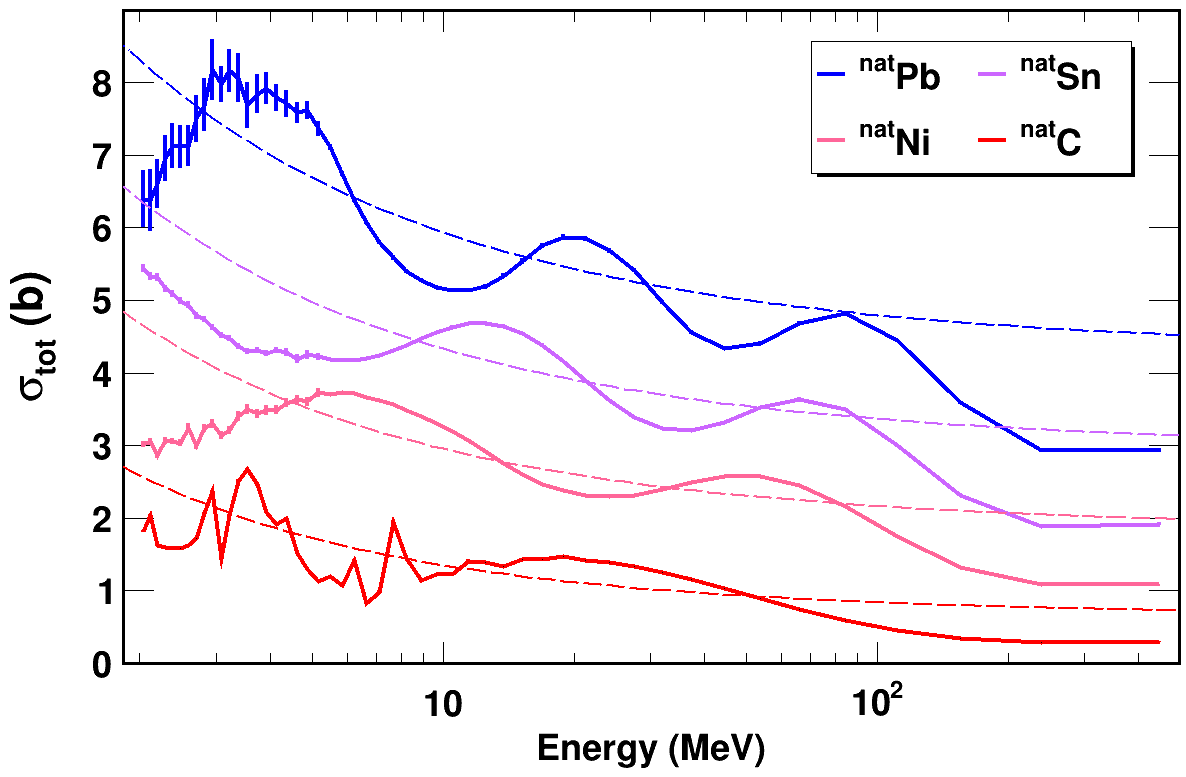
\includegraphics[width=0.5\textwidth]{figures/ExampleTCS.png}
    \caption{
        (Color online) Experimental \tot\ data are shown from 2-500
        MeV for nuclides from A=12 to A=208
        \cite{Finlay1993, Schwartz1974, Poenitz1983, Abfalterer2000, Abfalterer2001}.
        Predictions for \tot\ given by the ``strongly-absorbing sphere'' (SAS)
        model, Eq. \ref{SASAbsolute}, are shown as thin dashed lines for each nucleus.
        Regular oscillations about the SAS model are visible
        as is the trend for the oscillation
        maxima and minima to shift to \textit{higher} energies as A is increased.
    }
    \label{SASphereVsExperiment}
\end{figure}
Peterson \cite{Peterson1962} interpreted these oscillations as the 
result of a phase shift between neutron partial waves passing \textit{around} the 
nucleus (thus undergoing no phase shift) and waves passing
\textit{through} the nuclear potential, where they are refracted and exhibit a 
retardation of phase (an illustration is available in \cite{Satchler1980}).
This explanation was termed the 
``nuclear Ramsauer effect'' by Carpenter and Wilson \cite{Carpenter1959} based on 
the analogous effect seen in electron scattering on noble gases.

Following Angeli and Csikai \cite{Angeli1970}, this explanation can be
incorporated into the strongly-absorbing sphere relations (Eq. \ref{SASAbsolute}) 
by addition of a sinusoidal term:
\begin{equation} \label{OscillatoryModel}
    \tot = 2\pi (R+\lambdabar)^{2}(1 - \rho \cos(\delta))
\end{equation}
where $\rho = e^{-\operatorname{Im}(\Delta)}$ and $\delta =
\operatorname{Re}(\Delta)$, $\Delta$ being the phase difference between a
partial wave traveling
around and traveling through the nucleus. The large amplitude of the
oscillations ($\rho$) suggests that elastic scattering accounts for a
significant fraction of the total cross section, in turn implying a 
larger mean free path for neutrons through the nucleus 
than might otherwise be expected in the absence of Pauli blocking
\cite{Mohr1955, Feshbach1958}.
Continuing, if we approximate the nucleus with a
real spherical potential of radius $R$ and depth $U$, the total phase shift $\delta$ is:
\begin{equation} \label{phaseShift}
    \delta =
    \frac{\overline{C}\left(\left[{\frac{E+U}{E}}\right]^{\frac{1}{2}}-1\right)}{\lambdabar}
\end{equation}
where $\overline{C} = \frac{4}{3}R$ is the average chord length through the
sphere \cite{Angeli1970}. Rearranging Eq. \ref{phaseShift} in terms of A and E and
discarding leading constants yields:
\begin{equation}
    \delta \propto A^{\frac{1}{3}}\times\left(\sqrt{E+U}-\sqrt{E}\right)
\end{equation}
This form reveals an important relation: as A is increased, to maintain constant 
phase $\delta$, E must also increase \cite{Satchler1980, Peterson1962}. 
This is contrary to a typical resonance condition where an integer number of wavelengths
are fit inside a potential; in that case, to maintain constant phase as A is increased,
E must be decreased. Thus these \tot\ oscillations have been referred to as
``anti-resonances'' or ``echoes'' \cite{Satchler1980, McVoy1967}.
Other authors \cite{Ahmad1973} have
exposed weaknesses in Angeli and Csikai's interpretation of
Eq. \ref{OscillatoryModel} and have provided a more general semi-empirical
equation for \tot. However, Eq. \ref{OscillatoryModel} is a valuable starting
point for connecting \tot\ with the depth and shape of the nuclear
potential as experienced by neutrons.

By including additional surface, spin-orbit, and other terms, optical models (OMs) have been 
used to successfully reproduce the general features of all manner of single-nucleon scattering 
data across the chart of nuclides up to several hundred MeV \cite{Perey1976,
CH89, KoningDelaroche}. However, despite the excellent agreement with experiment, optical models
involve the interaction of many partial waves with many sometimes-opaque terms
in the potential, complicating intuitive understanding of the underlying
physics at play. In particular, the isovector components of optical potentials
are quite difficult to constrain as they depend on both proton and neutron 
scattering data, one or both of which are often unavailable. For example,
analysis of of neutron total cross section differences in W isotopes by Dietrich et al.
\cite{Dietrich2003} indicated that inclusion of standard isovector terms in the optical model they used
actually did a poorer job reproducing the W relative difference data, an
illustration of how poorly these isovector components are known.

With these considerations in mind, our present goal is twofold: first, to
provide new isotopically-resolved \tot\ data useful for identifying the 
dependence of optical 
potential terms on nuclear asymmetry; and second, conduct a Dispersive Optical Model
(DOM) analysis of these new \tot\ data along with a large corpus of scattering
and bound-state data to extract structural quantities (neutron skin
thicknesses, spectroscopic factors) for several cornerstone, closed proton shell nuclei.
This work details the experimental effort while the key findings of the DOM analysis are
presented in the companion paper \cite{Pruitt2020PRL}.

%from  Anderson and Grimes were the first to define an isospin-isospin cross section
%$\sigma_{is}$:
%\begin{equation}
%    \sigma = \frac{\sigma_{tot}^{>} - \sigma_{tot}^{<}}{2}
%\end{equation}
%where > and < refer to the isospin parallel ($T_0 + \frac{1}{2}$) and
%anti-parallel ($T_0 - \frac{1}{2}$) projections, with the explicit intention of
%examining the differences in \tot\ between isotopes to learn more about the
%isovector components of the optical potentials \cite{Anderson1990}.

\section{Experimental Considerations}
By scattering secondary radioactive beams off of hydrogen targets in inverse
kinematics, proton-scattering experiments are possible even on highly unstable
nuclides. Because neutrons themselves must be generated as a
secondary radioactive beam, neutron-scattering experiments are restricted to
normal kinematics and \tot\ measurements are possible only for relatively stable
nuclides that can be formed into a target. At present, \tot\ measurements above
the resonance region on nuclides with short half-lives (shorter than the timescale of
days) are technically infeasible for this reason, though a handful have been carried out on
samples with half-lives in the tens to thousands of years \cite{Poenitz1983,
Phillips1980, Foster1971}.

Traditionally, \tot\ measurements have relied on analog techniques for recording
events, techniques that suffer from a large per-event deadtime of
up to several $\micro\second$. Thus for a typical intermediate-energy \tot\ measurement
with dozens or hundreds of energy bins, achieving statistical uncertainty at the
level of 1\% requires a thick sample to attenuate a sizable fraction of the
incident neutron flux. For cross sections in the 1-10 barn range, this means
sample masses of tens of grams \cite{Finlay1993, Abfalterer2001}.
Producing an isotopically-enriched sample of this size is often
prohibitively expensive; indeed, a literature search for isotopically-resolved
\tot\ measurements reveals a paucity of data from 1-300 MeV, even for
closed-shell isotopes of special importance like $^{3,4}$He, $^{64}$Ni, and
$^{204}$Pb (see Table \ref{IsotopicCrossSectionTable}).


Recent developments in waveform digitizer technology have made it
possible to reduce the per-event deadtime by an order of magnitude or more,
enabling a corresponding reduction in the necessary sample size. In 2008, with
these improvements available, we
embarked on a campaign of \tot\ measurements on isotopically-enriched samples,
starting with $^{40,48}$Ca from $15 \leq E_{n} \leq 300$ MeV \cite{Shane2010}.
The data from that measurement have been incorporated into a comprehensive
Dispersive Optical Model (DOM) analysis \cite{Mueller2011, Mahzoon2014,
MahzoonPhDThesis} yielding proton and neutron spectroscopic factors, charge
radii, and initial estimates of the neutron skins \cite{Mahzoon2017}
for these nuclei.
Here we advance that program with \tot\ results for
the important closed-shell nuclides
$^{16,18}$O, $^{58,64}$Ni, and $^{112,124}$Sn. We also present a measurement
on a very thin sample of the naturally-monoisotopic $^{103}$Rh to demonstrate that
\tot\ experiments over a broad energy range using minute amounts of material are feasible.

\section{Experimental Details}
All \tot\ measurements were carried out at the 15R
beamline at the Weapons Neutron Research (WNR) facility of the Los Alamos
Neutron Science Center (LANSCE) during two run cycles (November 2016 and
September 2017). Our experiment was modeled on previous
\tot\ measurements at WNR \cite{Finlay1993,Abfalterer2001,Shane2010}.
At WNR,
broad-spectrum neutrons up
to $\approx$700 MeV are generated by impinging proton pulses onto a water-cooled, 7.5
cm-long tungsten target (see Fig. \ref{ExperimentalApparatus}). Before the beam
enters the experimental area, a
permanent magnet deflects all charged particles generated by the proton pulses, 
allowing only neutrons and $\gamma$ rays to reach the flight path. At the
entrance to the flight path, the beam was collimated to 0.200 inches using steel
donuts with a total thickness of 24 inches and hardened using a plug of Hevimet (90\% W, 6\% 
Ni, 4\% Cu by weight) inserted at the upstream entrance of the
collimation stack. After collimation, the beam passed successively through a flux 
monitor, the sample of interest held in a sample changer, a veto detector, and finally the 
time-of-flight (TOF) detector approximately 25 meters from the neutron source.
All detectors consisted of BC-400 fast scintillating plastic mated with 
photomultiplier tubes (PMTs) and encased in either a plastic or
an aluminum housing. The flux monitor and veto detector each had
scintillator thicknesses of $\frac{1}{4}$ inch and the TOF detector had a
scintillator thickness of 1 inch. Signals from all detectors and
the target changer were relayed to a 500-MHz CAEN DT-5730 waveform digitizer
running custom software. To improve time resolution, the TOF detector used two
PMTs (one left, one right) mated to the plastic scintillator and the PMTs' signals were 
summed before digitization.

\begin{figure}
    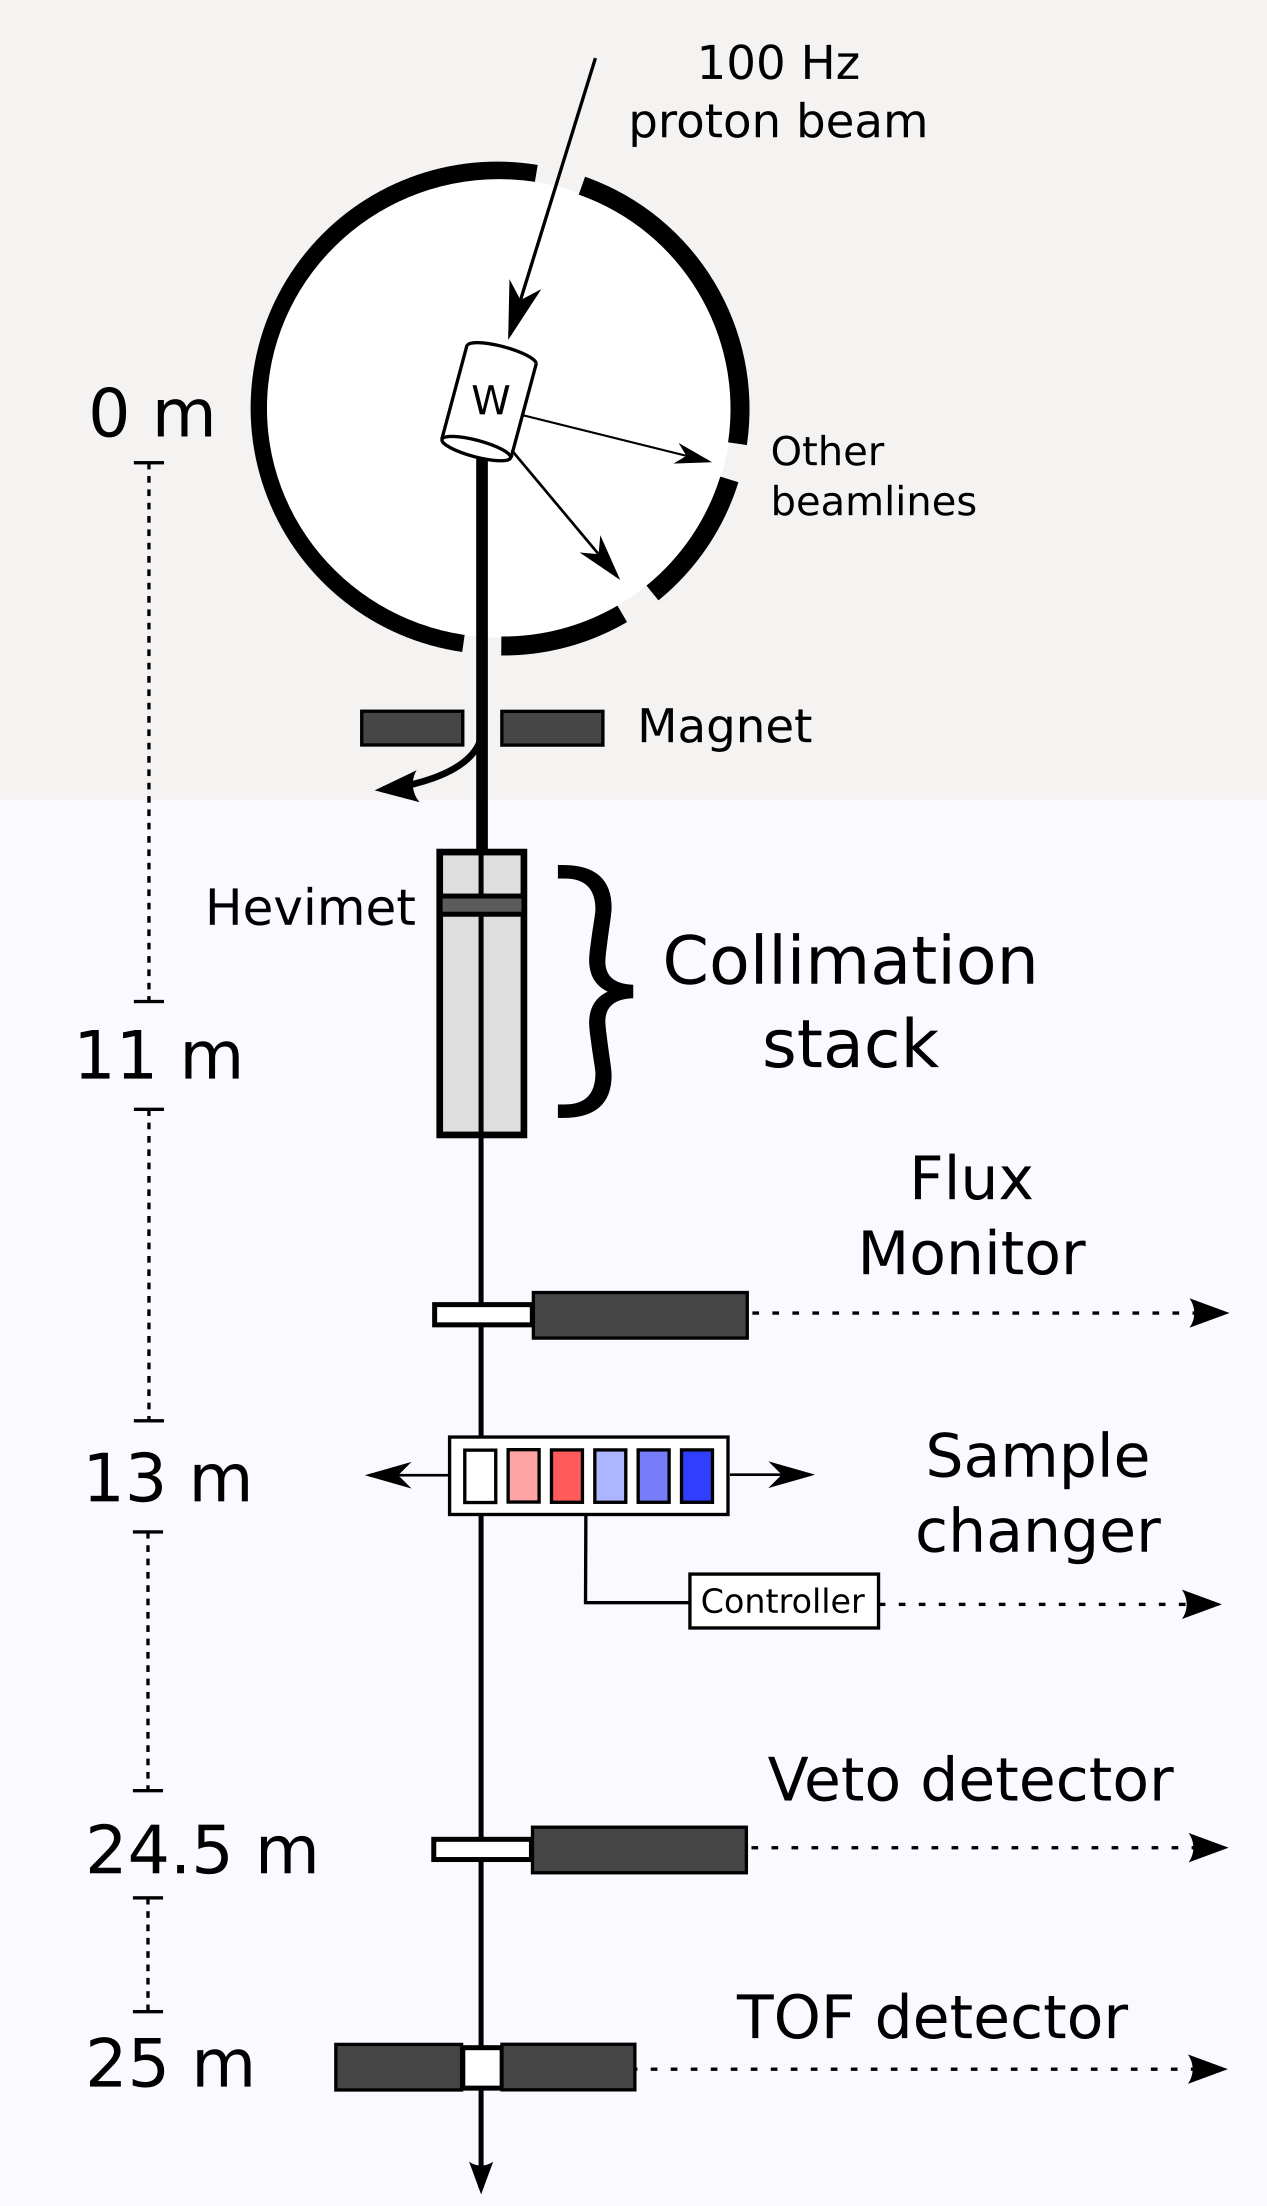
\includegraphics[width=0.3\textwidth]{figures/ExperimentalSetup.png}
    \caption{(Color online) Experimental configuration at WNR facility.
        Samples are cycled into and out of the beam
        using a linear actuator with a period of 150 seconds. Times-of-flight (TOFs) are
    determined by the TOF detector and used to calculate neutron energy.}
    \label{ExperimentalApparatus}
\end{figure}

\begin{figure}
    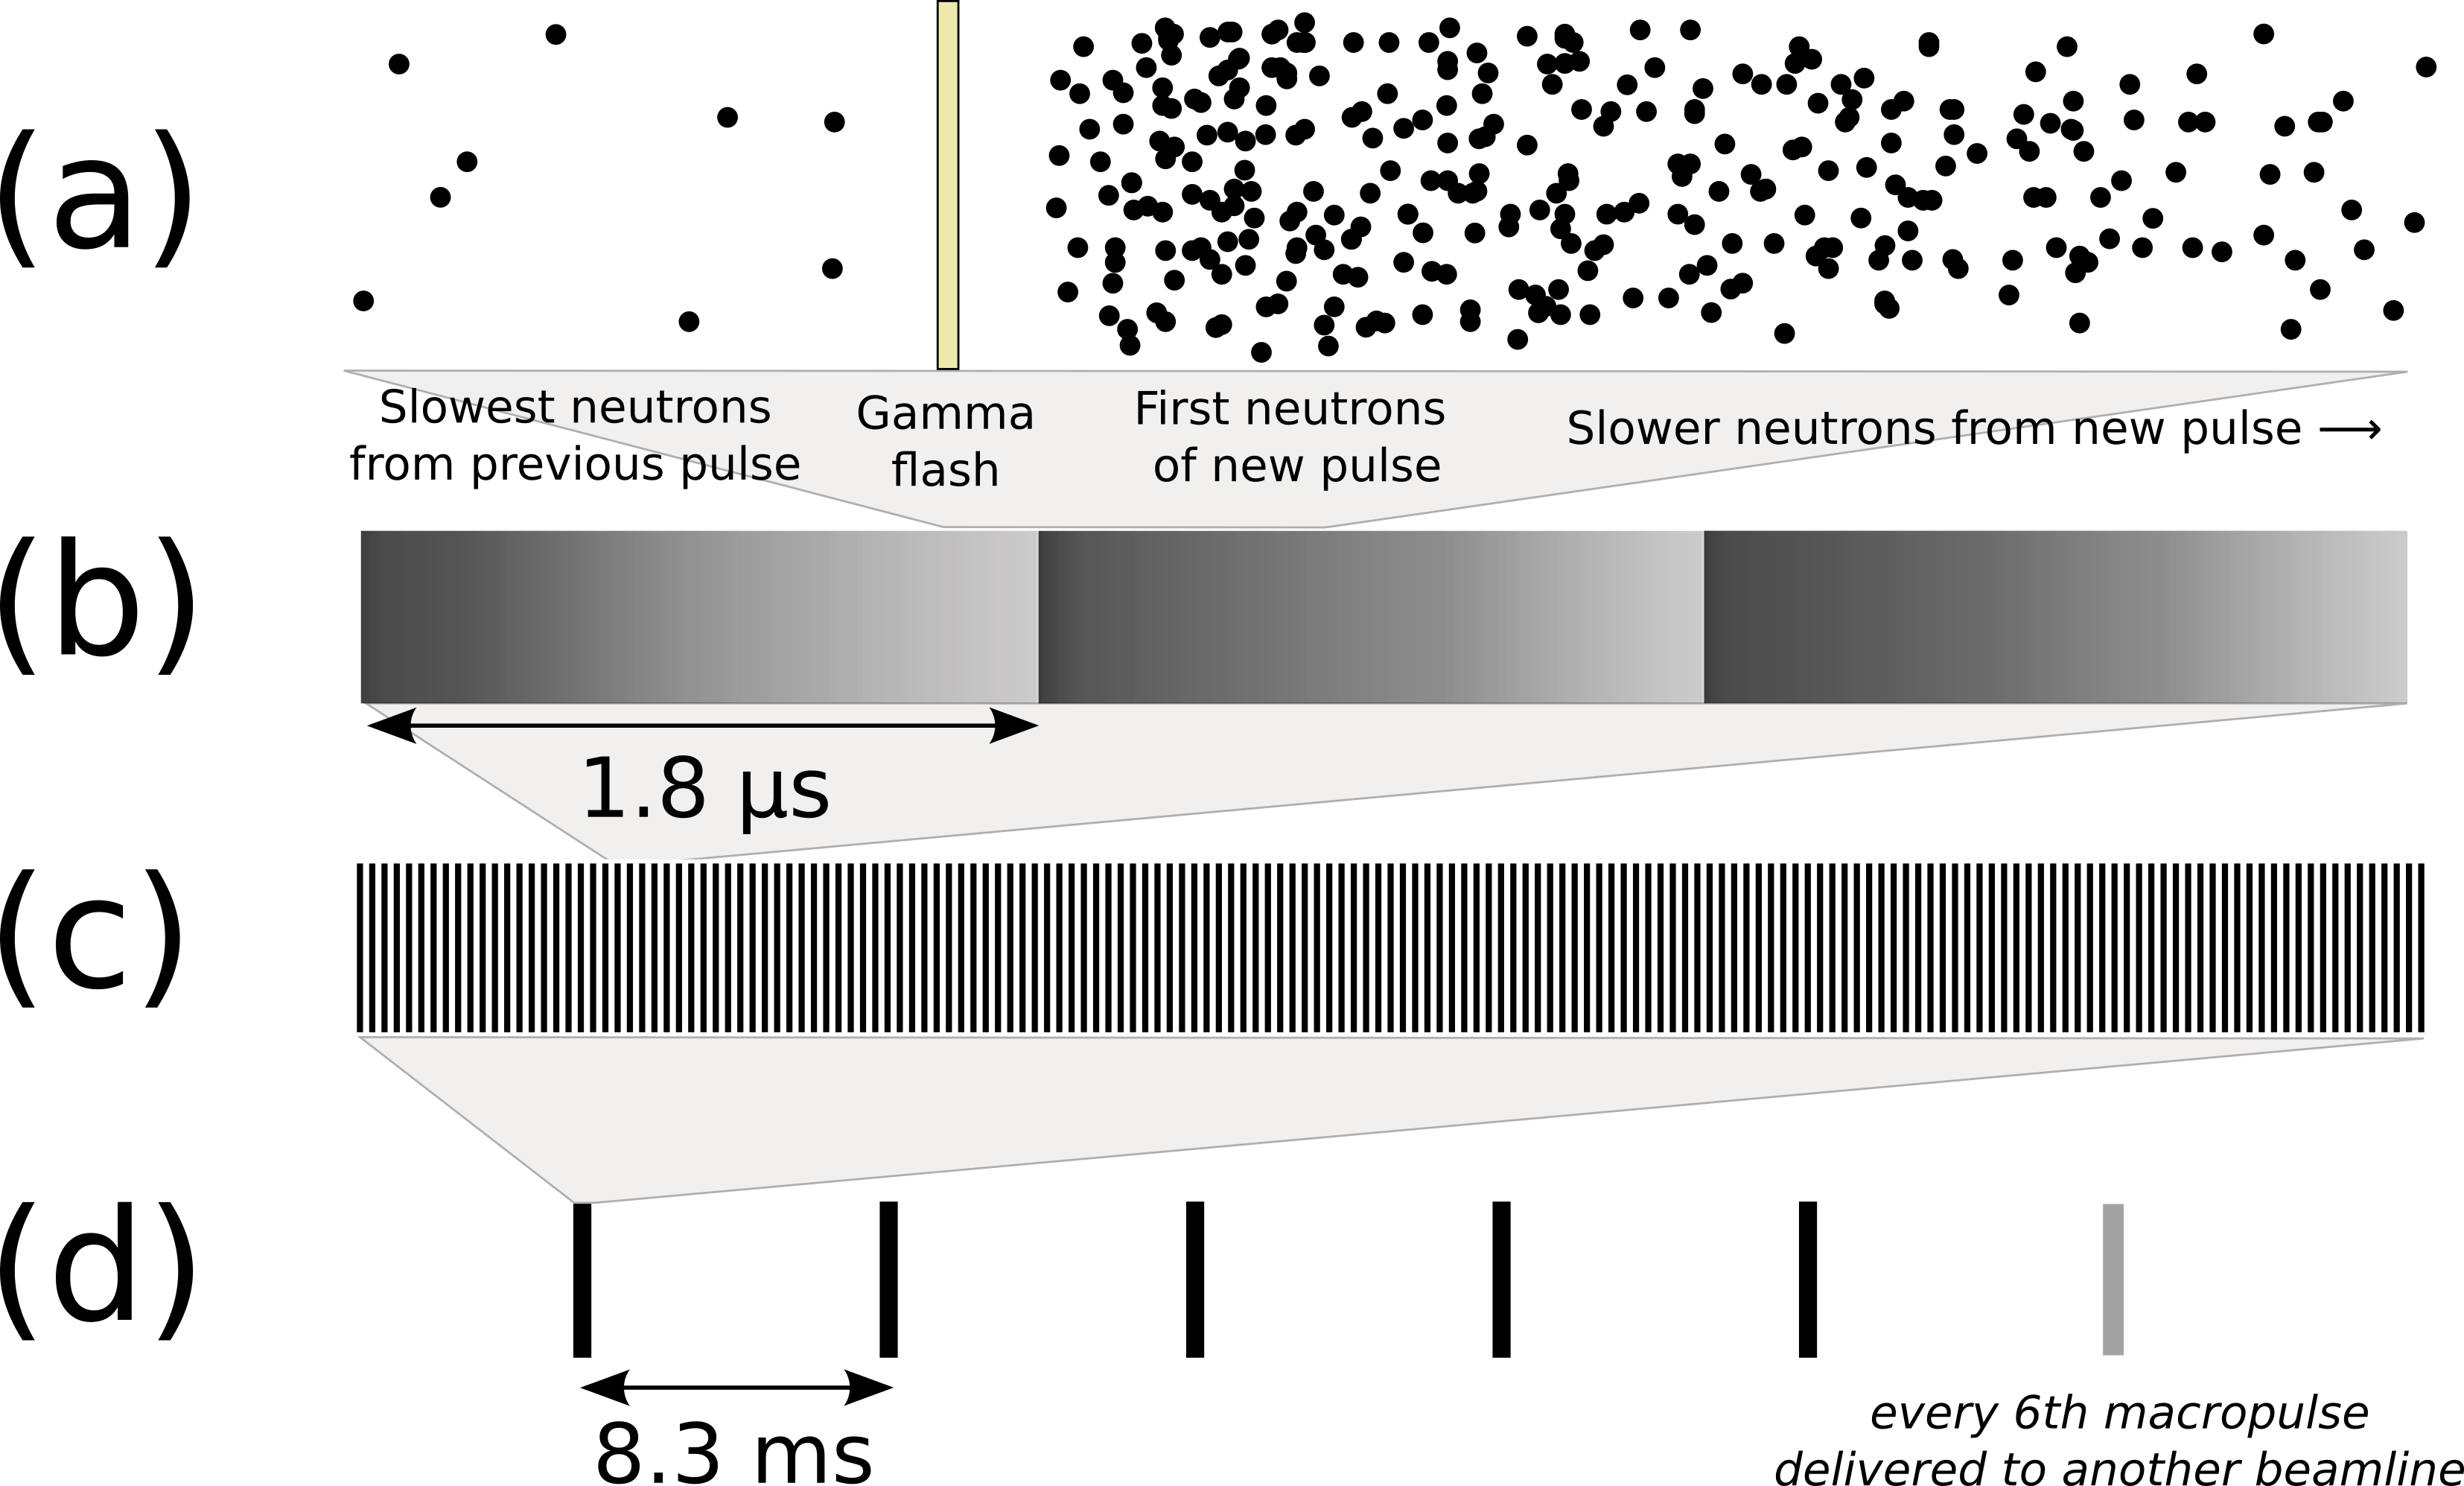
\includegraphics[width=0.5\textwidth]{figures/beamStructure.png}
    \caption{(Color online) Neutron beam structure at WNR facility.
        ``Macropulses'' of protons (row d) are delivered to
        WNR's tungsten Target 4, where they generate neutrons by spallation.
        Each macropulse consists of
        $\approx$350 proton ``micropulses'' (row c). Neutrons
        from each micropulse (row b) disperse in
        time as they travel along the flight path so that $\gamma$ rays and high-energy 
    neutrons catch up to low-energy ones from the previous pulse (row a).}
    \label{BeamStructure}
\end{figure}

The particular neutron beam structure at WNR dictates the energy range
achievable for \tot\ measurements (see Fig. \ref{BeamStructure}).
Proton pulse trains, called ``macropulses'', are delivered to the tungsten target at 120 Hz.
Each macropulse consists of ~350 individual proton pulses, called
``micropulses'', spaced 1.8 
$\mu$s apart. Each micropulse consists of a single proton packet $<$1 ns wide when it 
arrives at the tungsten target that generates $\gamma$ rays and neutrons within a tight
temporal-spatial range. As neutrons from this micropulse travel along the beam path, 
high energy neutrons separate in time from lower-energy neutrons so that neutron
energy can be determined by standard TOF techniques (see \cite{Moore1980} for details).
Because the $\gamma$ rays and high-energy neutrons from later micropulses can
overtake slower neutrons from an earlier micropulse, the distance of the TOF
detector from the neutron source determines both the minimum neutron energy that can be 
unambiguously resolved and the maximum instantaneous neutron flux, critical to correcting
for per-event deadtime.

A programmable sample changer with six positions
was used to cycle each sample into the beam at a regular interval of 150 seconds 
per sample. Once per macropulse, an analog signal from the sample changer
was recorded to indicate its current position.
The flux monitor was used to correct for variations in beam flux between 
macropulses. The veto detector suppressed events from charged-particle production 
in the samples and in air along the flight path.

Custom digitizer software was used to run the 
digitizer in two complementary modes, referred to as ``DPP mode'' and ``Waveform 
mode''. In DPP mode, triggers were initiated by the digitizer's onboard
peak-sensing firmware. For each trigger, several quantities were recorded: the trigger 
timestamp, two charge integrals over the detected peak with different
integration ranges (32 ns for the short integral, 100 ns for the long integral),
and a 96-ns portion of the raw digitized waveform, referred to as a ``wavelet''.
DPP mode was used for the vast majority of the 
experiment and accounts for $\approx$99\% of the total data volume. In waveform mode, 
the digitizer performs no peak-sensing and was externally triggered. Upon 
triggering, the trigger timestamp and a very long wavelet (60 $\micro\second$) 
were recorded. While waveform mode data accounts for only $\approx$1\% of the total data, 
the instantaneous data rate is much higher than in DPP 
mode because hundreds of $\micro\second$ of consecutive waveform samples are 
stored. Roughly once every three seconds, the digitizer was switched to 
waveform mode for one macropulse, then switched back to DPP mode as quickly as
possible (10-40 ms, depending on run configuration).  

Except for the oxygen and rhodium samples, all samples were prepared as right
cylinders 8.25 mm in diameter and ranging from 10-27 mm in length (see
Table \ref{SampleCharacteristics} for sample characteristics and Fig. \ref{SamplesImage}
for sample images). For each element under study, a natural-abundance sample
was also prepared as were two natural carbon
samples and a natural lead sample, useful for benchmarking against
literature data. The samples
were inserted into styrofoam sleeves and seated in the cradles of the sample
changer. This design minimizes the amount of non-target mass proximate to the
neutron beam path.

\begin{table*}[tb]
    \caption[Physical characteristics of samples used for neutron \tot\
    measurements]
    {
        For isotopically-enriched samples, the natural abundance
        of the enriched isotope and the isotopic fraction of the sample are
        given. To calculate cross sections, the relevant ``sample thickness'' is the areal
        density of nuclei $\rho_{\text{areal}}$, equivalent to
        the (volumetric) density times the length of the sample. For liquid
        samples H$_{2}^{\text{nat}}$O, D$_{2}^{\text{nat}}$O, and H$_{2}^{18}$O,
        the length and diameter listed are for the interior of the vessels
        used to hold the samples and the masses given are calculated based on 
        literature values for the density of each sample at 25 C.
        Our samples are generally much smaller than those used in previous
        measurements; for comparison, the Ni and Sn samples used in \cite{Abfalterer2001,
        Finlay1993} had areal densities of 1.515 and 0.5475
        $\frac{mol}{cm^{2}}$, respectively (12.7 and 6.5 times larger than our
        Ni and Sn samples). Columns 6 and 7 give the natural abundance of the
        isotope (NA) and the purity of our isotopic samples (SP).
    }
    \label{SampleCharacteristics}
    \begin{center}
        \begin{tabular}{ c c c c c c c }
            \hline
            Isotope & Len. [\milli\meter] & Diam. [\milli\meter]
            & Mass [\gram] & $\rho_{\text{areal}}$
            [$\frac{mol}{cm^{2}}$] & NA [\%] & SP 
            [\%]\\
            \hline

            $^{\text{nat}}$C & 13.66(2) & 8.260(5) & 1.2363
            & 0.1921(1) & - & -\\
            $^{\text{nat}}$C & 27.29(2) & 8.260(5) & 2.4680
            & 0.3835(2) & - & -\\
            \\
            H$_{2}$$^{\text{nat}}$O & 20.00(1) & 8.92(1) & 1.2461 & 0.1107(3) & - &
            - \\
            D$_{2}$$^{\text{nat}}$O & 20.00(1) & 8.92(1) & 1.3852 & 0.1107(3) &
            0.02 &
            99.9 \\
            H$_{2}$$^{18}$O & 20.00(1) & 8.92(1) & 1.3844 & 0.1107(3) & 0.20 &
            99.9\\
            \\
            $^{58}$Ni & 7.97(3)& 8.18(2) &
            3.6438 & 0.1197(3)& 68.1 & 99.6 \\
            $^{\text{nat}}$Ni & 8.00(3) & 8.20(2) &
            3.6898 & 0.1192(3)& - & -\\
            $^{64}$Ni & 7.96(2) & 8.20(4) &
            3.9942 & 0.1192(6) & 0.93 & 92.2\\
            \\
            $^{103}$Rh & 2.03(1) & 10.20(2) & 2.8359 & 0.02426(4) & 100 & 99.9\\
            \\
            $^{112}$Sn & 13.65(3) & 8.245(5) &
            4.9720 & 0.08332(5) & 0.97 & 99.9\\
            $^{\text{nat}}$Sn & 13.68(3) & 8.245(5) &
            5.3263 & 0.08414(5) & - & -\\
            $^{124}$Sn & 13.73(3) & 8.245(5) &
            5.5492 & 0.08399(5) & 5.79 & 99.9\\
            \\
            $^{\text{nat}}$Pb & 10.07(2) & 8.27(1) & 6.130 &
            0.05508(6) & - & -\\
            \hline
        \end{tabular}
    \end{center}
\end{table*}

%\begin{table*}[ht]
%    \caption{
%        Physical characteristics of all samples used for our \tot\
%        measurements. For isotopically-enriched samples, the natural abundance
%        of the enriched isotope and the isotopic fraction of the sample are
%        given. To calculate cross sections, the relevant ``sample thickness'' is the areal
%        density of nuclei $\rho_{\text{areal}}$, equivalent to
%        the (volumetric) density times the length of the sample. For liquid
%        samples H$_{2}^{\text{nat}}$O, D$_{2}^{\text{nat}}$O, and H$_{2}^{18}$O,
%        the length and diameter listed are for the interior of the vessels
%        used to hold the samples and the masses given are calculated based on 
%        literature values for the density of each sample at 25\textdegree{}C.
%        Our samples are generally much smaller than those used in previous
%        measurements; for comparison, the Ni and Sn samples used in \cite{Abfalterer2001,
%        Finlay1993} had areal densities of 1.515 and 0.5475
%        $\frac{mol}{cm^{2}}$, respectively (12.7 and 6.5 times larger than our
%    Ni and Sn samples).}
%    \label{SampleTable}
%    \begin{center}
%        \begin{tabular}{ c c c c c c c }
%            \hline
%            Isotope & Length & Diameter
%            & Mass & $\rho_{\text{areal}}$ & Nat. Abund. & Isotopic Purity\\
%                 & [mm] & [mm] & [g] & [$\frac{mol}{cm^{2}}$] & [\%] & [\%]\\
%            \hline
%
%            $^{\text{nat}}$C & 13.66(2) & 8.260(5) & 1.2363
%            & 0.1921(1) & - & -\\
%            $^{\text{nat}}$C & 27.29(2) & 8.260(5) & 2.4680
%            & 0.3835(2) & - & -\\
%
%            H$_{2}$$^{\text{nat}}$O & 20.00(1) & 8.92(1) & 1.2461 & 0.1107(3) & - &
%            - \\
%            D$_{2}$$^{\text{nat}}$O & 20.00(1) & 8.92(1) & 1.3852 & 0.1107(3) & - &
%            99.9 \\
%            H$_{2}$$^{18}$O & 20.00(1) & 8.92(1) & 1.3844 & 0.1107(3) & 0.20 &
%            99.0\\
%
%            $^{58}$Ni & 7.97(3)& 8.18(2) &
%            3.6438 & 0.1197(3)& 68.1 & 99.6 \\
%            $^{\text{nat}}$Ni & 8.00(3) & 8.20(2) &
%            3.6898 & 0.1192(3)& - & -\\
%            $^{64}$Ni & 7.96(2) & 8.20(4) &
%            3.9942 & 0.1192(6) & 0.93 & 92.2\\
%
%            $^{103}$Rh & 2.03(1) & 10.20(2) & 2.8359 & 0.02426(4) & 100 & 99.9\\
%
%            $^{112}$Sn & 13.65(3) & 8.245(5) &
%            4.9720 & 0.08332(5) & 0.97 & 99.9\\
%            $^{\text{nat}}$Sn & 13.68(3) & 8.245(5) &
%            5.3263 & 0.08414(5) & - & -\\
%            $^{124}$Sn & 13.73(3) & 8.245(5) &
%            5.5492 & 0.08399(5) & 5.79 & 99.9\\
%
%            $^{\text{nat}}$Pb & 10.07(2) & 8.27(1) & 6.130 &
%            0.05508(6) & - & -\\
%
%            \hline
%        \end{tabular}
%    \end{center}
%\end{table*}

The oxygen isotopes were prepared as water samples to increase the areal density
of atoms and for ease of handling. Each water sample was contained by a
cylindrical brass vessel with thin (0.002 inch) brass endcaps. Oxygen cross sections were calculated by
subtracting the well-known hydrogen cross section from the raw H$_{2}$O result
(we used H \tot\  data sets from Clement et al. \cite{Clement1972} and Abfalterer
et al. \cite{Abfalterer2001}, which together cover the range $0.5 \leq E_n \leq 500$ MeV
and are in excellent agreement where their energy ranges overlap). In light of
the additional uncertainty inherent to this kind of subtractive \tot\ determination,
a D$_{2}^{\text{nat}}$O sample from which the literature \tot\  for
D$_{2}$ could be subtracted was prepared as an additional cross-check. Due to
rhodium's poor machining properties, the \rhThree\ sample
was prepared by purchasing and stacking a series of thin discs rather than by
manufacturing a fused cylinder. These discs were corralled
by a cylindrical plastic case with open ends.

The sample configuration for each run varied, but generally all six positions on
the sample changer were used. For the solid targets, a typical configuration was
to place an empty styrofoam sample sleeve in the first sample-changer cradle as
the ``blank'', the $^{\text{nat}}$C and $^{\text{nat}}$Pb samples in the second and third
cradles, and the samples of interest (e.g., $^{58}$Ni, $^{\text{nat}}$Ni, $^{64}$Ni) in
the fourth, fifth, and sixth cradles. For water samples, an empty brass vessel
was placed in the first cradle to serve as the blank.

\begin{figure}
    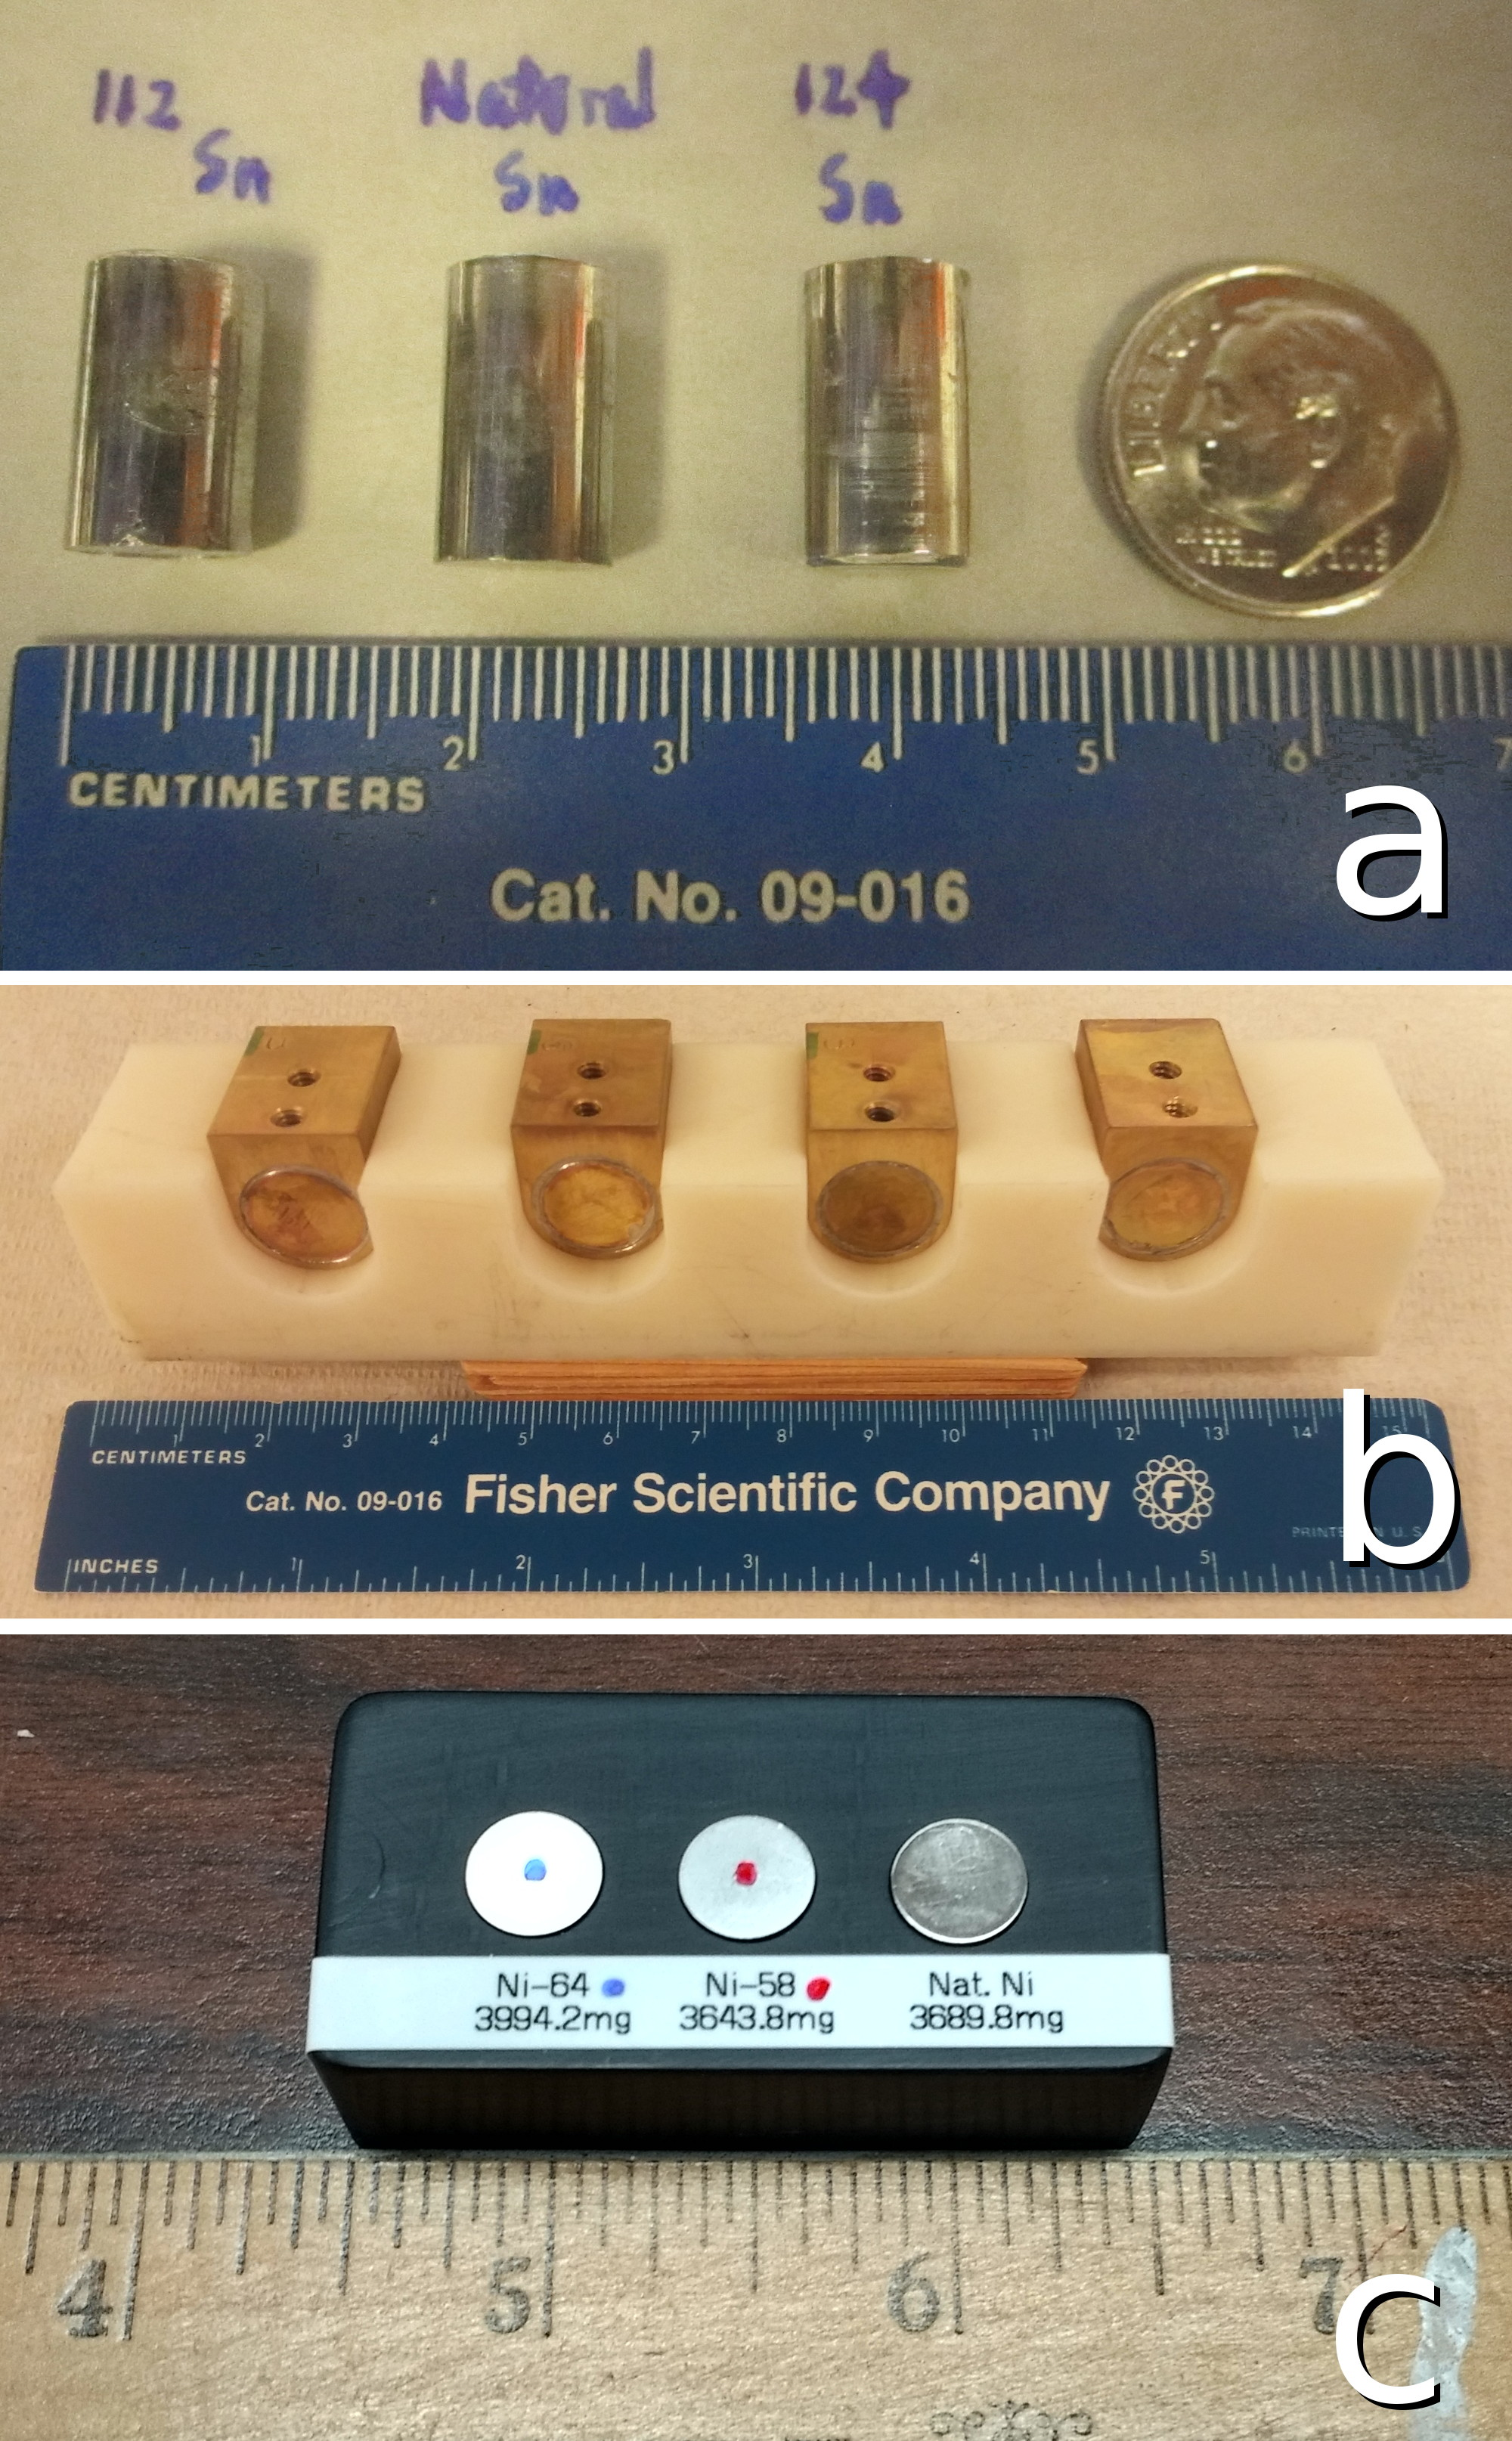
\includegraphics[width=0.3\textwidth]{figures/AllIsotopicSamples.jpg}
    \caption{(Color online) Section (a): the ${^{112,nat,124}}$Sn samples. Section (b): the 
        vessels used to hold water samples for the ${^{nat, 18}}$O \tot\  measurement. 
        Section (c): ${^{58,nat,64}}$Ni samples, shown end-on.}
    \label{SamplesImage}
\end{figure}

\section{Experimental Analysis}

The fundamental quantity of interest, \tot, is related to the flux
loss through a sample by:
\begin{equation}
I_{t} = I_{0}e^{-{\ell\rho\sigma_{tot}}}
\end{equation}
or, equivalently,
\begin{equation}
    \tot = -\frac{1}{\ell\rho}ln\left(\frac{I_{t}}{I_{0}}\right)
\end{equation}
where $I_{0}$ is the neutron flux entering the sample, $I_{t}$ is the neutron
flux transmitted through the sample without interaction, $\rho$ is the number
density of nuclei in the sample, and $\ell$ is the sample length. For thin
or low-density samples, flux attenuation through the sample will be small
(e.g., 13\% for our Ni samples at 100 MeV) and a large number
of counts will be required to determine the cross section to high
precision.

To identify valid neutron events and precisely determine the TOF start (micropulse start 
time) and TOF stop time (arrival at TOF detector) for each event, a series of corrections 
are required.  First, each event was assigned to the correct macropulse.
Time offsets accounting for cable and
electronics delay were applied, coarsely synchronizing all detectors with
facility-provided pulses indicating the arrival time of proton micropulses on the
tungsten target, so-called ``\tZero'' pulses.
To improve the time resolution for each TOF
event, the digitized waveform for each event was passed 
through an offline software constant-fraction discriminator (CFD) algorithm
and a $\gamma$-ray-averaging
procedure (cf. \cite{Shane2010}) was used to improve the precision of the start 
time of each micropulse.  After these corrections, the final TOF resolution
(taken as the FWHM of the $\gamma$-ray peak in the TOF spectra) ranged from
0.60-0.90 ns over the series of \tot\ measurements.
This is comparable to the resolution from 
our digitizer-mediated \tot\ measurement on Ca isotopes in 2008 \cite{Shane2010}.
For context, for a 100-MeV neutron and a TOF detector distance of 27 meters, a TOF 
uncertainty of 0.80 ns translates to an energy resolution of $\approx$900 keV.
For neutrons below $\approx$20 MeV, the TOF time resolution worsens as the traversal time 
through the 1-inch thickness of the TOF detector becomes non-negligible.
However, because the TOF of these neutrons is already several hundred ns or
longer, the relative energy resolution ($\frac{\Delta E}{E}$) is
superior at low energies: for a 5 MeV neutron with a 0.82 ns detector-traversal time and
an inherent TOF resolution of 0.80 ns, $\Delta E$ is 13 keV. These energy uncertainties
have been propagated through subsequent analysis into our \tot\ results below.

Calculating the neutron energy requires knowledge of the flight path
distance to high precision. We determined this distance by calculating 
putative \tot\ data for $^{\text{nat}}$C from 3-15 MeV from our measurement and 
comparing the resonance peaks in this region with high-precision literature data
sets. From this study, the TOF distance was determined as 2709 $\pm$1
\centi\meter\ for the Ni and Rh run configuration and 2554
$\pm$1 \centi\meter\ for the Sn and O run configuration.

\begin{figure}
    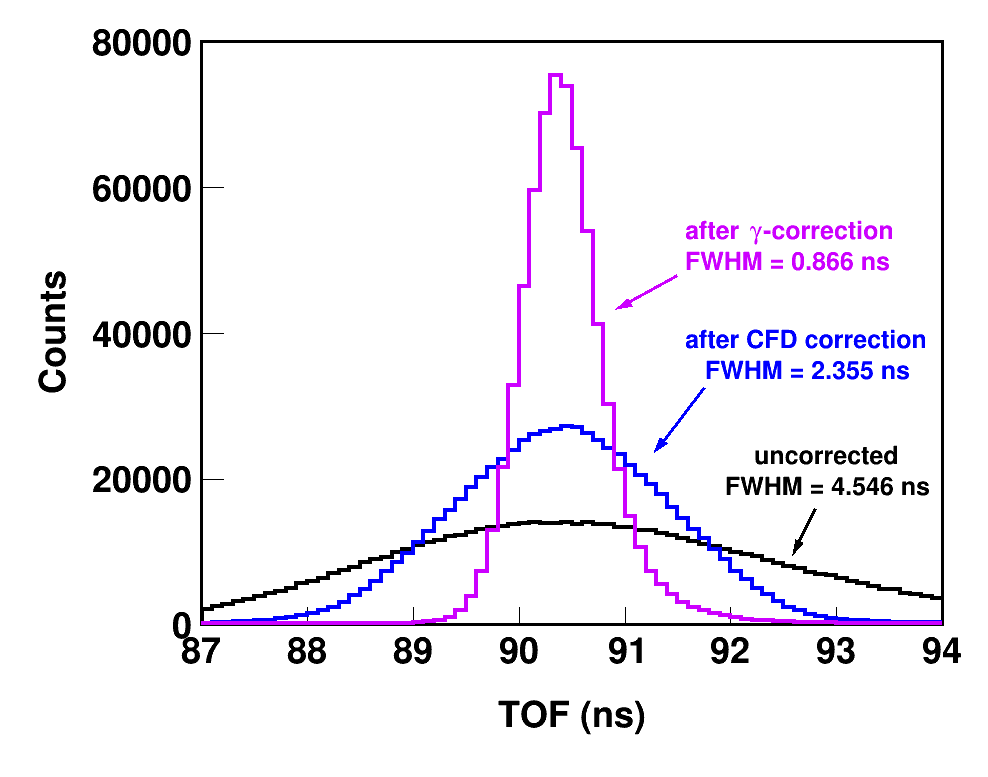
\includegraphics[width=0.5\textwidth]{figures/TimeCorrections.png}
    \caption{(Color online) The effects of timing corrections on the $\gamma$-ray
        peak of a typical run are shown. The uncorrected spectrum is shown in black,
        the spectrum after correction with our software CFD is shown in blue,
        and the spectrum after correction with both our software CFD and
        $\gamma$-averaging is 
        shown in pink. For this run, the final $\gamma$-ray peak 
        FWHM after both corrections is 0.866 ns, comparable to the precision we
        achieved in our Ca study \cite{Shane2010}, which also employed $\gamma$-
        averaging.
        }
    \label{TimingCorrectionStudy}
\end{figure}

Before cross sections could be tabulated, the per-event deadtime had to be
modeled and corrected for. Because events are not processed
instantaneously, there is a brief period
after each trigger during which the digitizer is busy processing that trigger.
Any newly-arriving events in this period will be ignored,
privileging events arriving earlier and thus distorting
TOF spectra and resulting cross sections. This busy period is referred to as the
``analytic'' or ``per-event'' deadtime and can be corrected for according to standard 
techniques
\cite{Moore1980}. An additional complication is the possibility of flux
variation between micropulses. If there is no variation, the fraction of time
that the digitizer is dead for a given time bin $i$ can be calculated with a
simple formula, per Moore's analysis of rate-dependence of counting losses
\cite{Moore1980}:
\begin{equation}
    F_{i} = \sum^{N-1}_{j=0} R_{(i-j)\text{ mod N}}\times P_{j}
    \label{DeadtimeEquation}
\end{equation}
where $N$ is the number of time bins in the micropulse, $R_{x}$ is the rate of
detected events per micropulse in bin $x$, and $P_{j}$ is the probability that the
digitizer is still busy from a trigger $j$ bins ago.
Moore also provides a more advanced formula to generate the appropriate
dead-time correction in cases where the variation in beam flux 
is significant. However, an examination of our flux-per-micropulse data showed
very little flux variance across macropulses, except during the first 10\%
of the micropulses within each macropulse. In our final analysis, we discarded 
the first 40 micropulses of each 
macropulse and used the simpler Eq. \ref{DeadtimeEquation} to calculate the dead
time fraction.

To model the experimentally-observed $P_{j}$, we
employed a logistic function and fitted it to the observed spectrum for time
differences between consecutive events (see Fig.
\ref{TimeDifferenceBetweenEvents}). For a given bin $i$, the fraction of time that the 
digitizer is dead, $F_{i}$, is in essence a discrete convolution of the
\textit{measured} TOF spectrum with $P_{j}$. Note that except for the first and
last micropulses in a macropulse, micropulses are consecutive and thus deadtime effects can
``wrap around'' from the end of one micropulse to the next. For these wrap-around
contributions (that is, $j>i$), the (mod N) term ensures that the bin referred
to by $i-j$ is non-negative and has physical meaning as a time bin from the 
previous micropulse.

\begin{figure}
    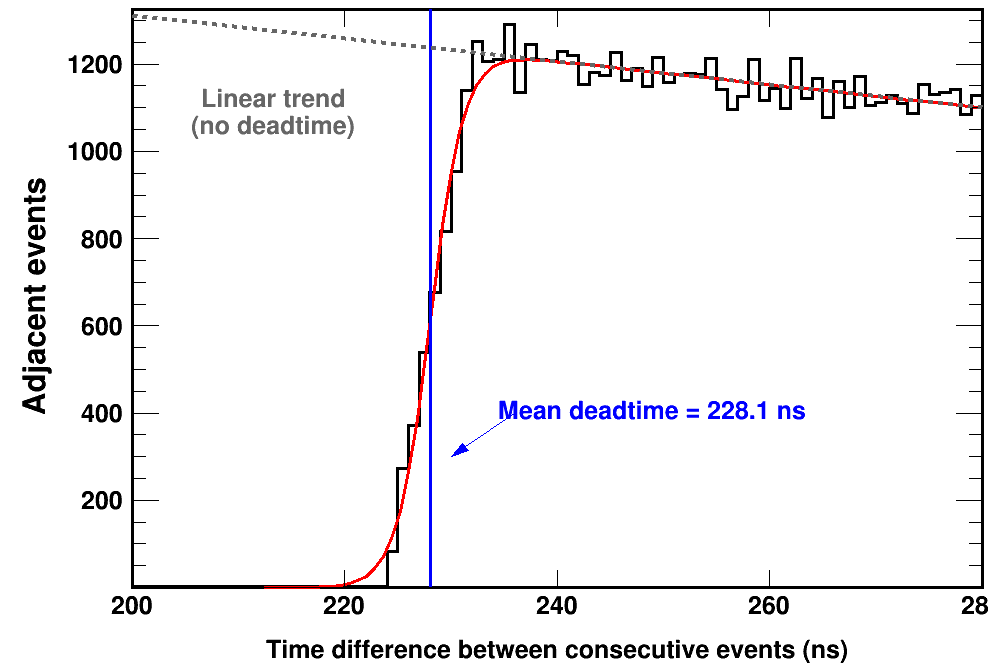
\includegraphics[width=0.5\textwidth]{figures/TimeDifferenceBetweenEvents.png}
    \caption{(Color online) The time difference between adjacent TOF-detector
    events for a single run is plotted (black histogram). Below a certain
minimum time difference (the ``deadtime''), no events are recorded. A logistic
fit (red) models the detector's deadtime response and is used to generate a
deadtime correction. The underlying linearly-decreasing count rate (gray dashed
line) in incorporated into the logistic model. From the fit, a mean deadtime of
228.1 ns was extracted for the Sn and O run configurations (a similar
procedure was used to recover a deadtime of 159.7 ns for the Ni and Rh
run configurations).}
    \label{TimeDifferenceBetweenEvents}
\end{figure}

Because trigger processing is done in firmware onboard the digitizer,
the per-event deadtimes affecting our
measurement were reduced to between 150-230 \nano\second.
Once the average probability-dead was calculated for each time bin,
the total number of
events detected in that bin, $N_{d}[i]$, was corrected to the \textit{true}
number of events in that bin $N_{t}[i]$ that would have been detected in the
absence of a per-event deadtime:
\begin{equation}
    N_{t}[i] = -ln\left[1-\frac{\frac{N_{d}[i]}{M}}{(1-F_{i})}\right]\times M
\end{equation}
where M is the total number of micropulse periods. At large TOFs (low energies) 
the correction is as low as a few percent,
but at small TOFs (high energies) when the digitizer is still dead
from the $\gamma$-ray flash and high-energy neutrons, the correction is 
significant ($\approx$20\% for our Ni/Rh runs, and $\approx$40\% for
our Sn/O runs). These 
corrections are themselves far lower than the typical
analytic deadtime correction required with the deadtime mitigation scheme of
previous analog measurements \cite{Finlay1993,
Abfalterer2001}. %The effect of this correction on the final 
%cross section results is shown in Fig. \ref{DeadtimeEffectOnCS}.

In addition to analytic deadtime, there is an additional deadtime factor associated with 
digitizer readout to the data acquisition computer (DAQ). During data
collection, each pair of digitizer channels shares a common buffer for storing events.
After several seconds of acquisition, the digitizer tally of total events would
reach reaching a user-defined threshold to begin readout, at which time the
acquitision was paused and buffer contents passed out to the DAQ. However,
because each buffer was independently read out to the DAQ, it is possible that buffers
could be emptied and readied for new acquisition at slightly different times
(10-40 ms apart). Such run-time interactions between the firmware and USB
traffic of the DAQ were difficult to characterize, but we estimate that they might cause a 
systematic error of a few tenths of one
percent in the number of macropulses seen by differing channels, depending on the user-defined 
threshold and the buffer size, which could contribute to the discrepancy at the
highest energies ($>$100 MeV) between our results and past analog-enabled
measurements. 

During analysis, it was noted that occasionally (1 in 400 macropulses), one or two 
adjacent macropulses would have an abnormally small number of flux monitor events or 
TOF events. The frequency of these ``data dropouts'' was similar to the rate of
switching between DPP and waveform modes and we suspect it is related to edge
case behavior right before or after a mode switch. To mitigate this issue,
any macropulse that had less than 50\% of the average event rate in either the
flux monitor or TOF detector channel was ignored during cross section calculation.

After applying these corrections, the veto and integrated charge gates are applied to 
all events and surviving events are populated into TOF spectra (see Fig.
\ref{ExampleTOFSpectrum}). Next, room background was subtracted (responsible for 0.1\% to 
1\% of event rate, depending on energy) and spectra were mapped to the energy domain.

\begin{figure}
    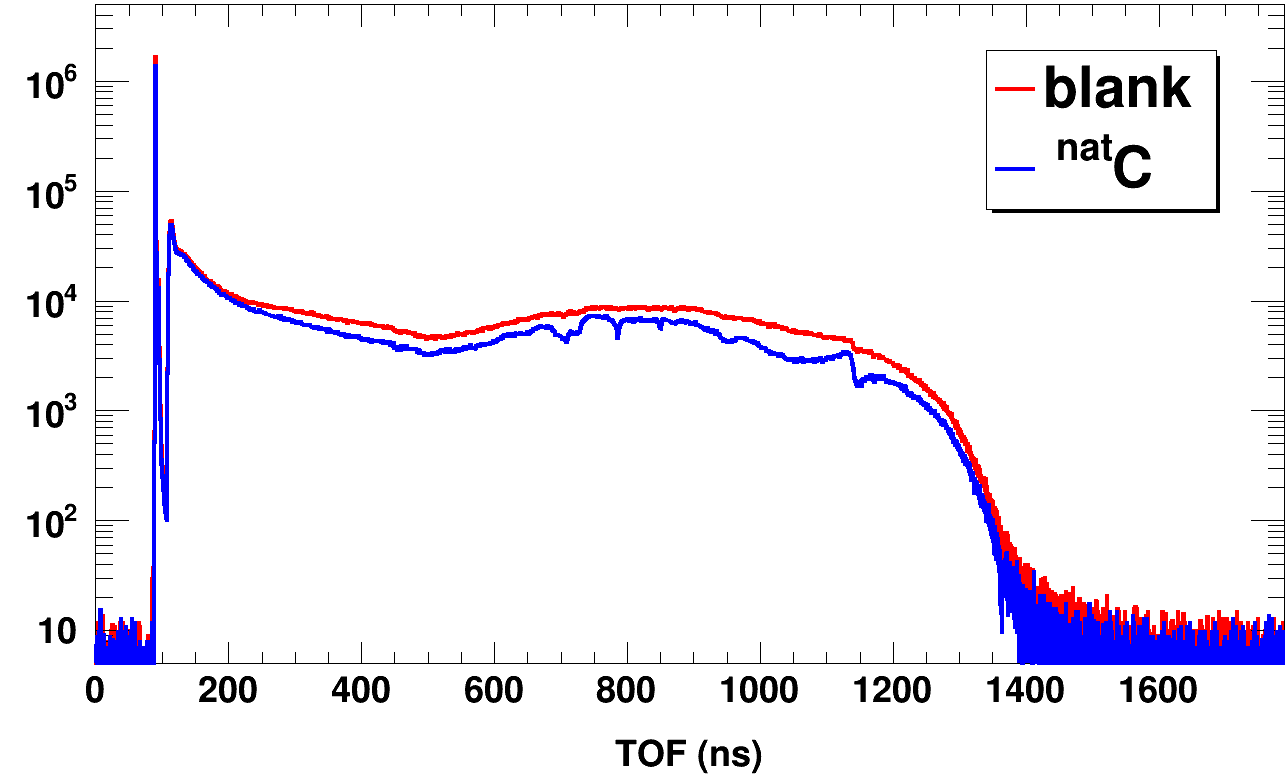
\includegraphics[width=0.5\textwidth]{figures/exampleTOFSpectrum.png}
    \caption{(Color online) TOF spectra after analytic deadtime correction and
        veto and integrated charge gating for the blank sample (in
        red) and for the $^{\text{nat}}$C sample (in blue), from the Ni/Rh experiment.
        The $\gamma$-ray peak is visible as a sharp spike at 90 ns, followed by
        the highest-energy neutrons at 130 ns. The small spikes spaced 60 ns
        apart (visible before 90 ns and after 1500
        ns) are identified as $\gamma$-ray peaks from a low-level, continuous
        ``drip'' 
        of protons onto the tungsten target caused by mistuning of the proton 
        buncher; their effect on the calculated cross sections is negligible.
    }
    \label{ExampleTOFSpectrum}
\end{figure}

From these energy spectra, the raw cross sections were calculated, bin-wise, as follows:
$$
\tot = -\frac{1}{\ell\rho_{n}}
\ln \left(\frac{I_{0}}{I_{s}}\times\frac{M_{s}}{M_{0}}\right)
$$
where $\frac{I_{0}}{I_{s}}$ is the ratio of counts in the energy spectra between 
the blank and sample, $\frac{M_{s}}{M_{0}}$ is the ratio of counts in the
monitor detector between the sample and blank (for flux normalization), $\ell$ is the length 
of the sample, and $\rho_{n}$ is the number density of atoms in the sample.

A series of small corrections were applied to the raw cross sections to produce
the final results. First, because the blank sample contains air and not vacuum,
the cross section of air must be added to each other sample's cross section (scaled by  
the ratio of areal densities of air in the blank and the sample of interest).
For the sample with the smallest areal density (Rh), this correction was 2 mb.
The cross section for $^{64}$Ni was corrected for the isotopic enrichment of our
sample (92.2\%) using our measured $^{\text{nat}}$Ni cross section. All other isotopes were 
sufficiently pure such that the impurity correction was negligible.

To validate our analysis, we first benchmarked our \tot\ measurements of natural samples
($^{\text{nat}}$C, $^{\text{nat}}$Ni, $^{\text{nat}}$Sn, and
$^{\text{nat}}$Pb) against the high-precision data sets on natural samples from Finlay
\cite{Finlay1993} and Abfalterer \cite{Abfalterer2001}, shown in Fig.
\ref{LiteratureBenchmarking}. Our natural sample results
are in excellent agreement with 
these previous results from 3-100 MeV and show slight deviation above 100 MeV (a
relative difference of up to 5\% at 300 MeV), suggesting a small systematic
error at high energies in one or both approaches when the instantaneous neutron
flux is highest. As an additional diagnostic, we compared 
\tot\ results from our long and short natural carbon targets and
found excellent agreement, within 1\% throughout the measured energy domain.

Extracting the \oSixEight\ neutron \tot\ required subtraction of the
well-measured hydrogen neutron \tot. To better understand
the additional systematic uncertainty
associated with this subtractive analysis, we subtracted our final
\oSix\ neutron \tot\ results from our raw D$_{2}$O and H$_{2}$O data and 
calculated the deuterium-to-hydrogen neutron \tot\ relative difference. A
comparison of our D-to-H relative difference with that of
\cite{Abfalterer1998} is shown in the supplemental materials. Our results differ
systematically from the previous (analog) measurement by 2-3\% throughout the
energy range, comparable to the 2\% systematic difference between our final
\oSix\ neutron \tot\ results and those of \cite{Abfalterer2001}. The size and
uniformity of these systematic differences is consistent with
a combination of slight ($\approx$ 1\%) normalization errors
in some or all of the H, D, O, and C neutron \tot\ results,
both in our measurement and in the literature.

\begin{figure}
    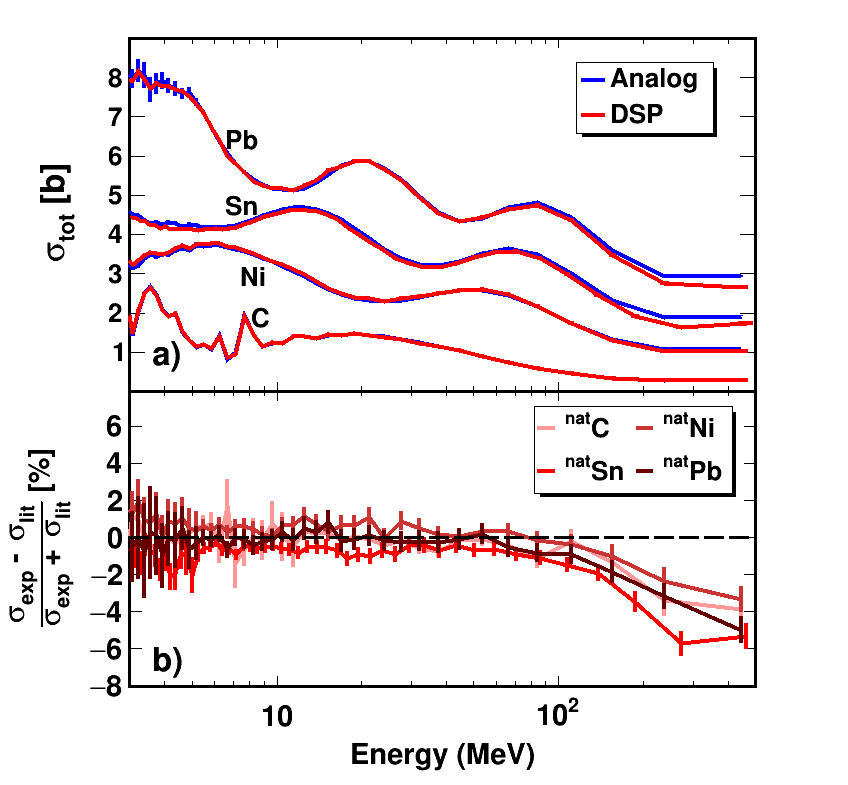
\includegraphics[width=0.5\textwidth]{figures/literatureBenchmarking.png}
    \caption{(Color online) A comparison of literature data (taken with analog
    techniques) and our results (signals processed with a digitizer, or ``DSP'')
    for natural C, Ni, Sn, and Pb. In panel (a), the absolute cross sections are shown from
    3-500 MeV; in panel (b), the relative differences between the literature data and
    our data are shown in percent. From 3-100 MeV, our data are fully consistent with the
    literature datasets but above 100 MeV, a difference arises, peaking at
    $\approx$5\% at 300 MeV.
b}
    \label{LiteratureBenchmarking}
\end{figure}

\section{Experimental Results}

Our absolute \tot\ results for O, Ni, and Sn isotopic targets are shown in Fig.
\ref{SixPanel} (results for Rh are shown in the supplemental materials).
Literature isotopic \tot\ measurements
(where they exist) are shown alongside our results for comparison.
Residuals between our data and any existing literature data are also shown.
In each figure, the literature data sets have rebinned to match the bin
structure of our data to facilitate comparison. In regions with a low density of
states where individual resonances are visible (e.g., $^{\text{nat}}$C
below 10 MeV), this rebinning washes out the fine structure of the
cross section data.

Except for the already well-measured \oSix, our new data significantly
extend knowledge of the neutron \tot\ for each sample. In the case of \oEight,
\niEight, \rhThree, and \snFour, almost all previous data was collected at less 
than 20 MeV. Our new data are in reasonable agreement with the previous
measurements when experimental error of these measurements is taken into
account. In the cases of the rare isotopes \niFour\ and \snTwelve,
only one datum (at 14.1 MeV) was 
available in the literature \cite{Dukarevich1967}. Our measurements on these
rare isotopes are in excellent agreement, within 2-3\%, of these data from more
than fifty years ago.

Our results for relative differences between isotopic pairs \oSixEight,
\niEightFour, and \snTwelveFour\ are shown in Fig. \ref{ThreePanelRelDiff}. In
\oSixEight, the purely-isoscalar SAS model grossly reproduces the relative
difference below 100 MeV, but fails completely above 100 MeV. Near 200
MeV, the \oEight\ \tot\ drops below that of \oSix\ resulting in a negative
relative difference, in keeping with the Ramsauer-logic expectation (Eq.
\ref{OscillatoryModel}) that \tot\ oscillation minima shift to higher
energies as A is increased. In the relative difference subfigures for 
\niEightFour\ and \snTwelveFour, the average \tot\ values are below the
SAS model trend ($r \propto A^{\frac{1}{3}}$), shown by the black dashed lines. 
The well-known $r \propto A^{\frac{1}{6}}$ trend in Sn isotope shift data 
\cite{Anselment1986} are also shown for reference (grad dotted lines) and
underpredict the relative differences. As was noted by Dietrich et al. in
their study of \tot\ relative differences in W isotopes, a simultaneous optical
model analysis along the entire isotopic chain (a l\'a \cite{Mueller2010})
may be required to reproduce the oscillatory behavior seen in the relative differences.
The individual Dispersive Optical Model fits to \oSixEight, \niEightFour, and
\snTwelveFour\ in the following section lay the groundwork for a future study of
this type.

\begin{figure*}[tb]
    \centering
    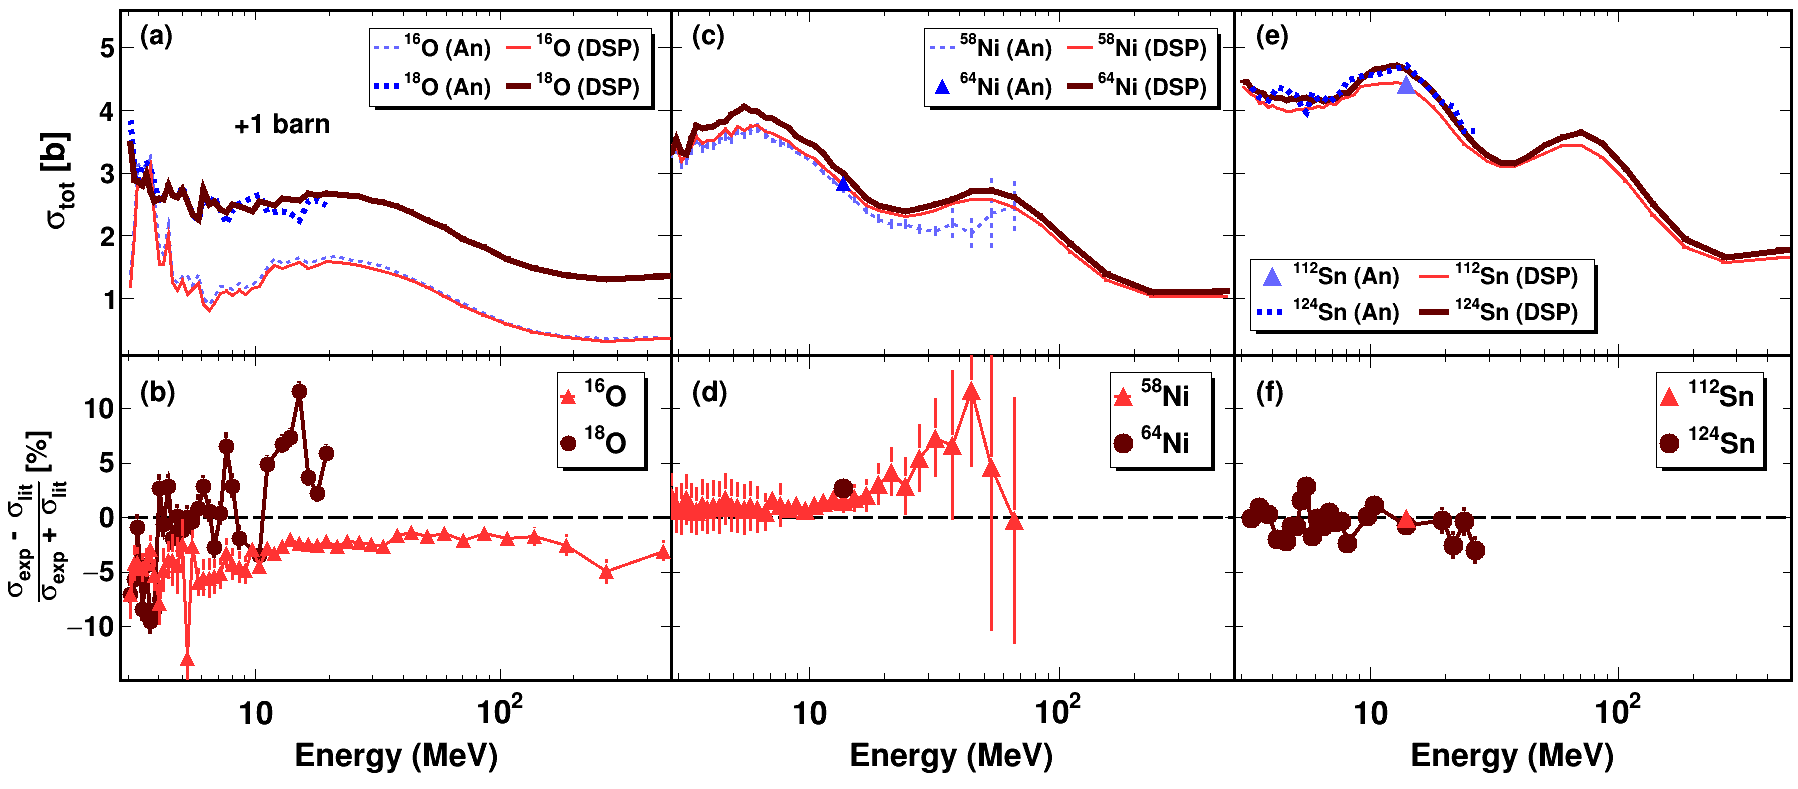
\includegraphics[width=\textwidth]{figures/SixPanel.png}
    \caption[Neutron \tot\ for \oSixEight, \niEightFour, and \snTwelveFour: our results and literature data]
    {(Color online) Neutron \tot\ for \oSixEight, \niEightFour, and \snTwelveFour: our results 
        and literature data.  In the upper three panels, our digitizer-measured
        isotopic results are shown in red and
        corresponding analog-measured literature data \cite{Finlay1993, 
        Perey1972, Vaughn1965, Salisbury1965, Perey1993, Dukarevich1967,
        Harper1982, Timokhov1989, Rapaport1980} are shown in blue.
        The data for \oEight\ in panel a) have been
        shifted up by 1 barn for visibility.
        The lower three panels show residuals between our data and the
        literature data shown in the upper three panels.
    }
    \label{SixPanel}
\end{figure*}

\begin{figure*}[tb]
    \centering
    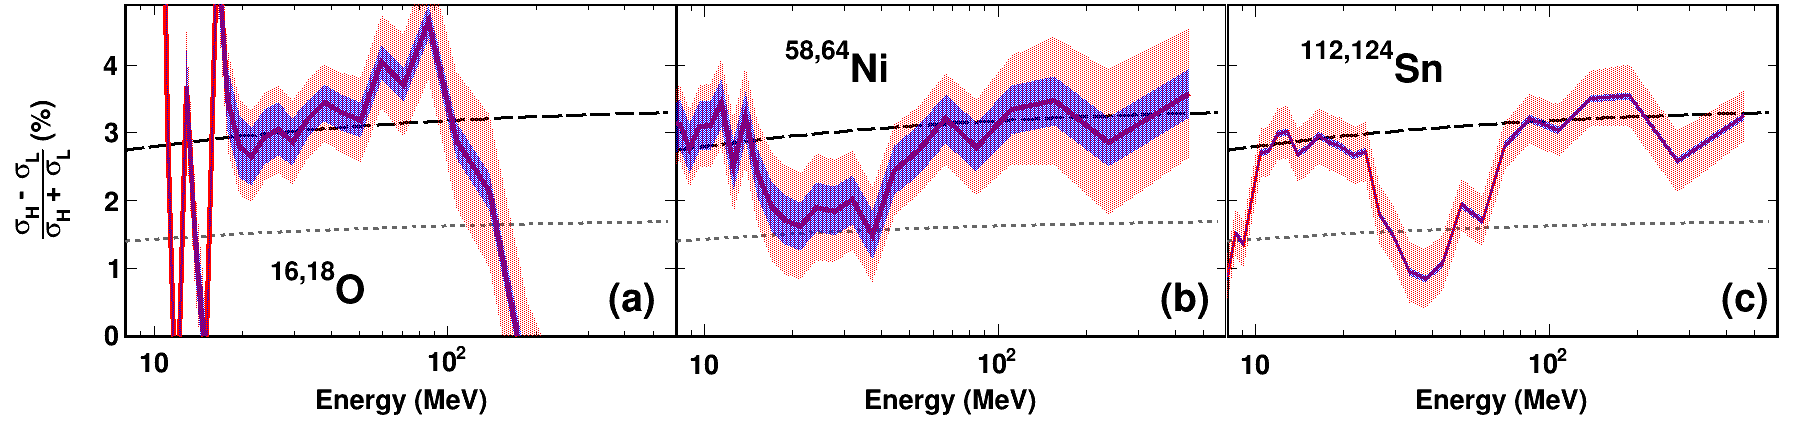
\includegraphics[width=\textwidth]{figures/ThreePanelRelDiff.png}
    \caption[\oSixEight, \niEightFour, \snTwelveFour\ neutron \tot\ relative difference]
    {
        (Color online) \oSixEight, \niEightFour, \snTwelveFour\ neutron \tot\ relative differences
        from our measurement. In each figure, the black dashed line shows the 
        prediction for the \tot\ relative difference per the strongly-absorbing 
        sphere (SAS) model (Eq. \ref{SASAbsolute}), which assumes a simple 
        A$^{\frac{1}{3}}$ size scaling for the nuclear radius.
        The gray dotted line shows the
        SAS model prediction but with an
        A$^{\frac{1}{6}}$ size scaling. The blue band in each panel indicates
        uncertainty due to target thickness imprecision;
        the red band in each panel
        indicates uncertainty from both target thickness and statistics.
    }
    \label{ThreePanelRelDiff}
\end{figure*}

\section{DOM Analysis}

The Dispersive Optical Model (DOM) is a phenomenological Green's-function
framework enabling a simultaneous and self-consistent analysis of nuclear
structure and reaction data.
An essential feature of the DOM is the enforcement of a dispersion
relation between the complex components of the self-energy across the entire
energy domain, allowing structural data from below the Fermi energy
(e.g., charge densities, bound levels) to constrain the potential above,
and data from above the Fermi energy (e.g., elastic, reaction, and total
cross sections) to constrain the potential
below. A thorough description of the DOM formalism and of past DOM analyses are
available in \cite{Mahaux1991, Dickhoff2018, PruittPhDThesis, AtkinsonPhDThesis, MahzoonPhDThesis}.

With our new \tot\ data for \oSixEight, \niEightFour, and \snTwelveFour, we
performed a comprehensive DOM analysis on these isotopes along with
\caAughtEight and \pbEight using Markov-Chain Monte Carlo
(MCMC) to optimize DOM parameters (see the companion paper
\cite{Pruitt2020PRL} for details on the MCMC implementation). Compared to previous DOM analyses
\cite{Mueller2011, AtkinsonPhDThesis, MahzoonPhDThesis}, we used an updated version of the DOM
that has been generalized for use with any even-even nucleus that is not too
deformed. Partial filling of open shells, as for the neutron $d_{\frac{5}{2}}$
valence shell in \oEight, is accommodated with a simple
pairing parameter $\Delta$ (details are provided in \cite{PruittPhDThesis}).
The full DOM potential parameterization and the optimized parameter mean values
and variances recovered from the fitting are provided in Appendix
\ref{ParameterValues} for all isotopes. The purpose of this section is to
demonstrate the suitability of the DOM approach (as evidenced by the quality of
the reproduction of experimental data used to constrain the potential) and to
identify the dominant gaps in the nuclear data available for these systems
and their impact on predicted quantities. Detailed results for \oSixEight\ are presented
in the following subsection, followed by summarized results for \niEightFour\ and
\snTwelveFour.

\subsection{Experimental data used to constrain $^{16}$O DOM potential}
Nucleon elastic scattering data (including differential cross sections and analyzing
powers) from 10-200 MeV and nucleon reaction cross sections from 20-65 MeV
were retrieved from the EXFOR database \cite{EXFORDatabase}.
For protons, twenty-eight elastic differential cross
sections data sets, twenty analyzing power data sets,
and three reaction cross section data sets were
incorporated in this energy range (see full list in Appendix
\cite{DataReferences}). Due to the lack of experimental proton
reaction cross sections between 65-200 MeV, we generated proton reaction cross
section data points based on systematic trends identified in the comprehensive
review of Carlson \cite{Carlson1996}. These pseudo-data points were included in the fit.
For neutrons, ten neutron elastic differential cross section
data sets, ranging from a neutron energy of 10 MeV to 95 MeV, and a single
neutron reaction cross section data point, at 14 MeV, were included. 
Our newly-measured \tot\ results for $^{16}$O were included as well. In all,
over sixty experimental nucleon scattering data sets, including our new \tot\ 
measurement, were used to constrain the \oSix\ parameters.

In addition to nucleon scattering data, several sectors of bound-state data were
included in the fit. Neutron (proton) 0p$_{\frac{1}{2}}$ and 0d$_{\frac{5}{2}}$
single-particle level energies were
assigned according to the nucleon separation energies of $^{16}$O and
$^{17}$O isotopes ($^{16}$O, $^{17}$F isotopes) \cite{AME2016}.
The charge density distributions used were extracted/compiled from elastic
electron scattering data \cite{DeVries1987}. Since the time of that compilation,
new experimental data (in particular from muonic atom measurements) have improved the precision
of many root-mean-square (RMS) charge radii by roughly an order of magnitude \cite{Angeli2013}.
To account for these improved data, we rescaled the distributions from
\cite{DeVries1987} to recover the updated
RMS charge radii while still conserving particle number. We also fitted directly
to the updated RMS charge radii of \cite{Angeli2013}.
Lastly, the experimentally-known total binding energy of \oSix\ from \cite{AME2016} was
included as a fit constraint. 

\subsection{Experimental data used to constrain $^{18}$O potential}
As with $^{16}$O, a large corpus of proton elastic scattering data was
available in the EXFOR database. Twenty-eight proton elastic differential cross
sections were include, with an energy range from 10-200 MeV in the lab frame.
No proton reaction cross sections were available. On the neutron side, two
elastic differential cross section data sets were used, at 14 and 24 MeV in the
lab frame. Only one data point for the neutron reaction cross section was available
(14.1 MeV) and was included. Our new \tot\ results for $^{18}$O were the
sole neutron total cross section data used in the fit. The energies of the
neutron (proton) 0p$_{\frac{1}{2}}$ and 0d$_{\frac{5}{2}}$ single-particle
levels were assigned according to the same procedure used for \oSix.

Unlike \oSix, for \oEight, no charge density distribution was available from
\cite{DeVries1987}. To approximate it, we re-scaled the charge density
distribution used for \oSix\ to match the reported \oEight\ RMS charge radius
while preserving 8 units of charge. As with \oSix, we also fitted to the
evaluated RMS charge radius of \cite{Angeli2013} and to the total binding
energy.

\subsection{Fit results on $^{16}$O}
\begin{figure*}[!htb]
    \centering
    \begin{minipage}{0.45\textwidth}
        \centering
        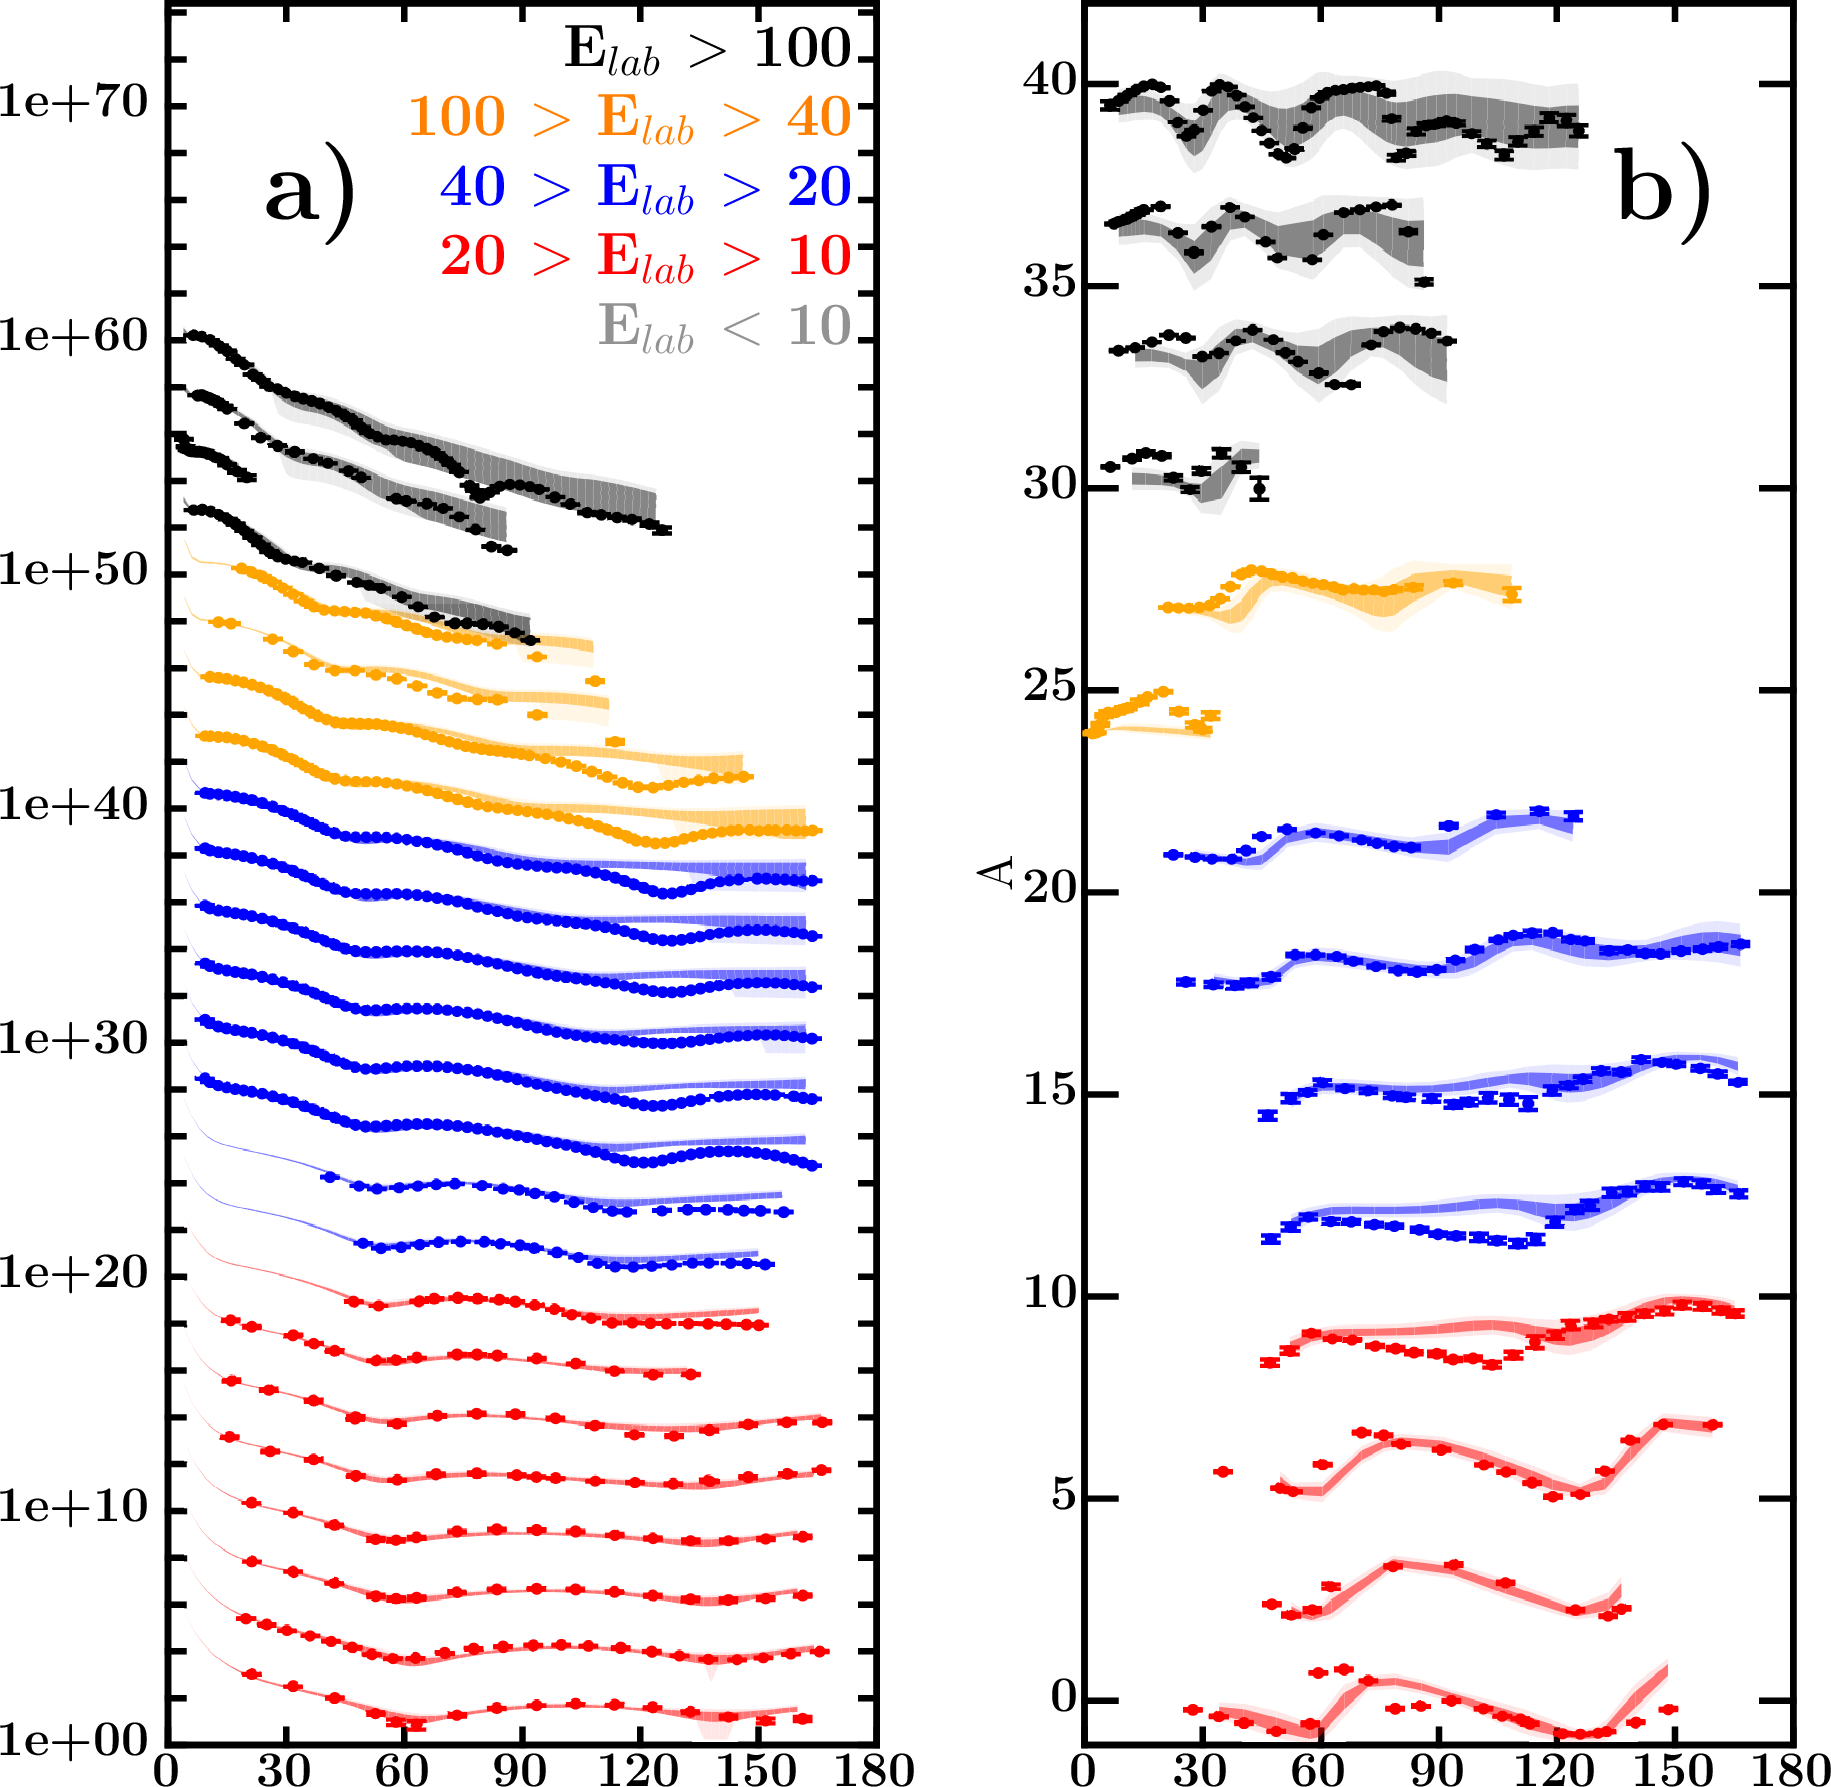
\includegraphics[width=\textwidth]{figures/o16_protonElastic.png}
        \label{DOM_o16_proton_elastic}
    \end{minipage}\hspace{6pt}
    \begin{minipage}{0.45\textwidth}
        \centering
        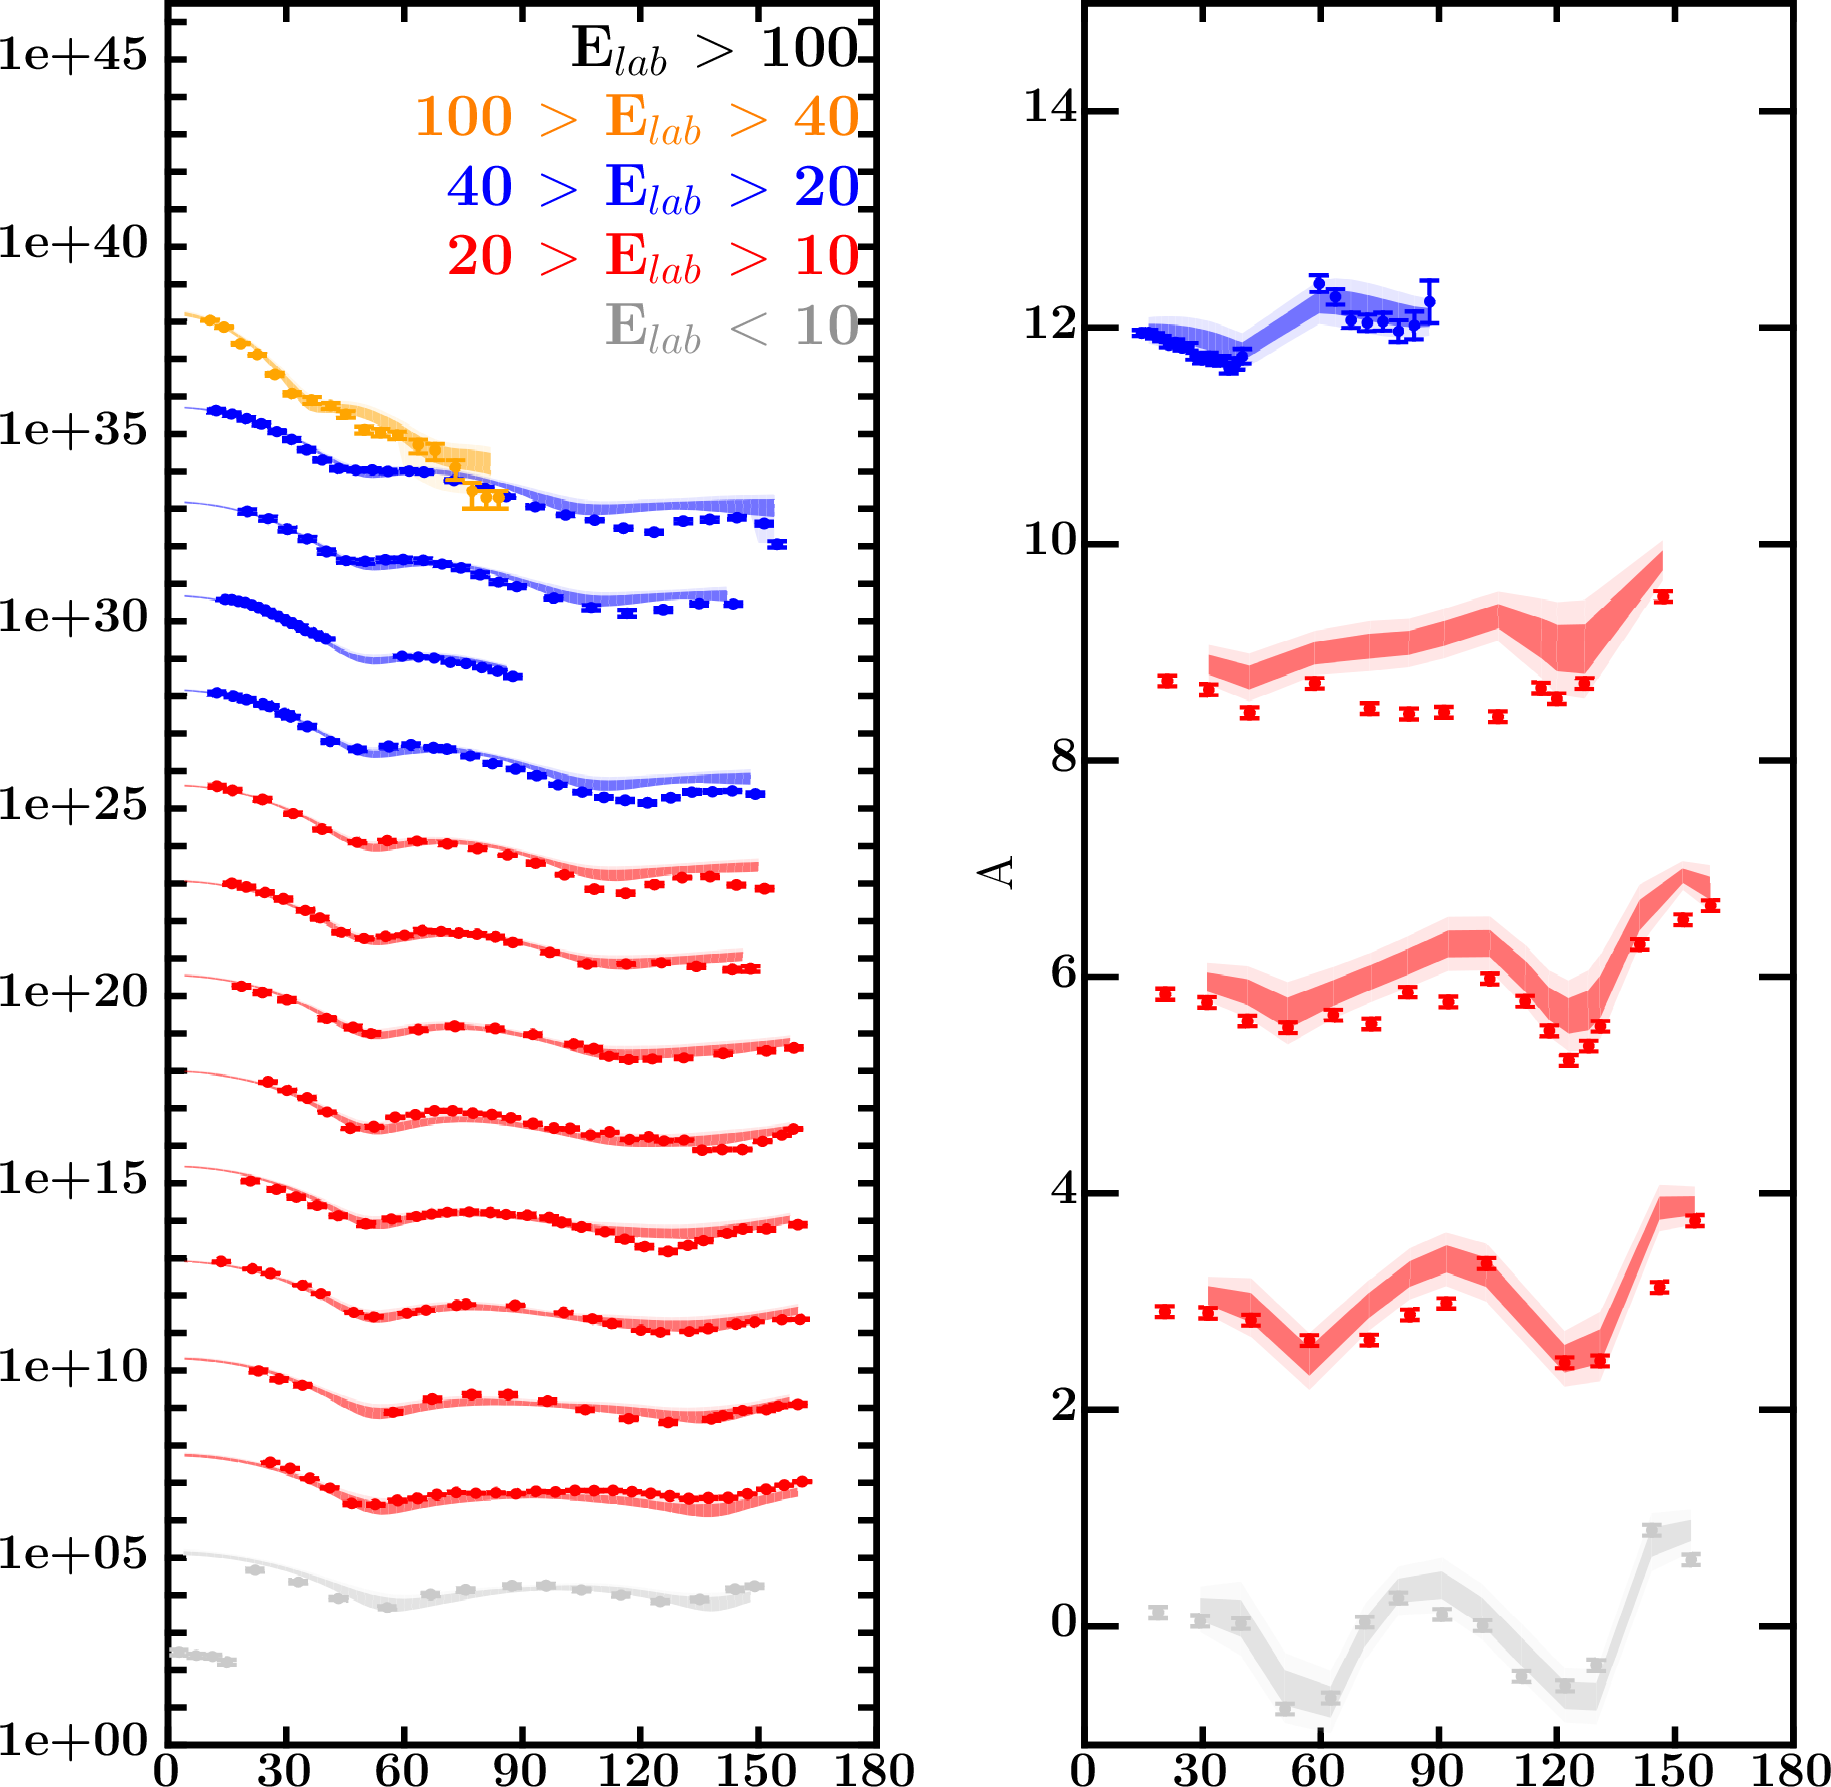
\includegraphics[width=\textwidth]{figures/o16_neutronElastic.png}
        \label{DOM_o16_neutron_elastic}
    \end{minipage}
    \centering
    \begin{minipage}{0.45\textwidth}
        \centering
        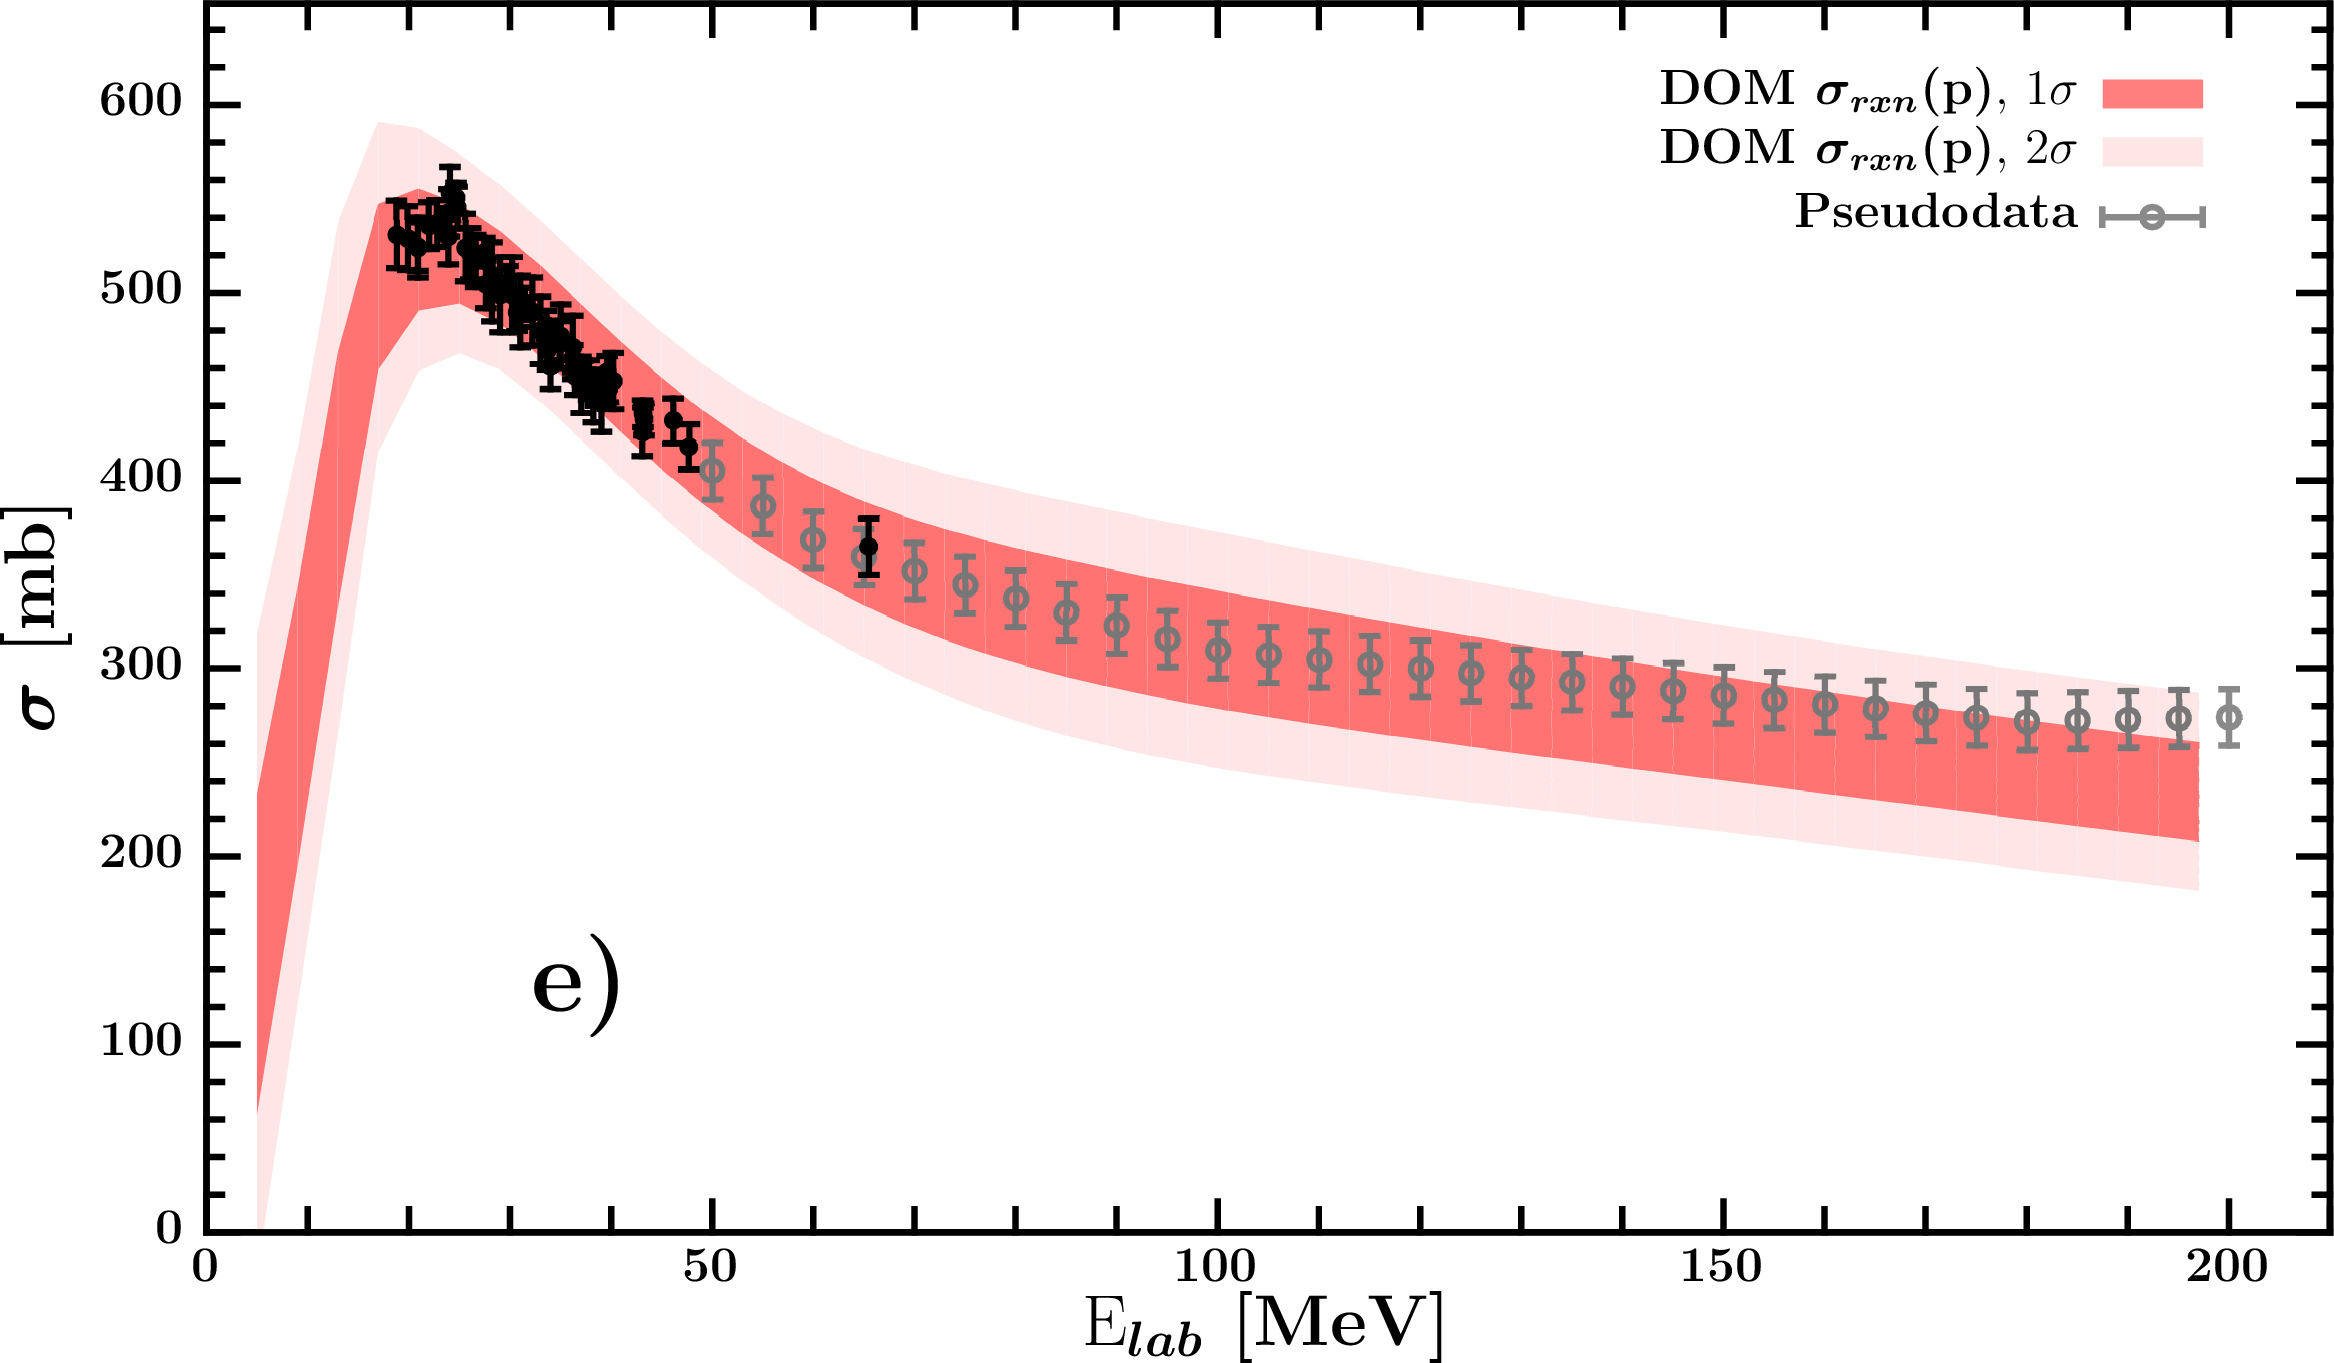
\includegraphics[width=\textwidth]{figures/o16_protonInelastic.png}
        \label{DOM_o16_proton_inelastic}
    \end{minipage}\hspace{6pt}
    \begin{minipage}{0.45\textwidth}
        \centering
        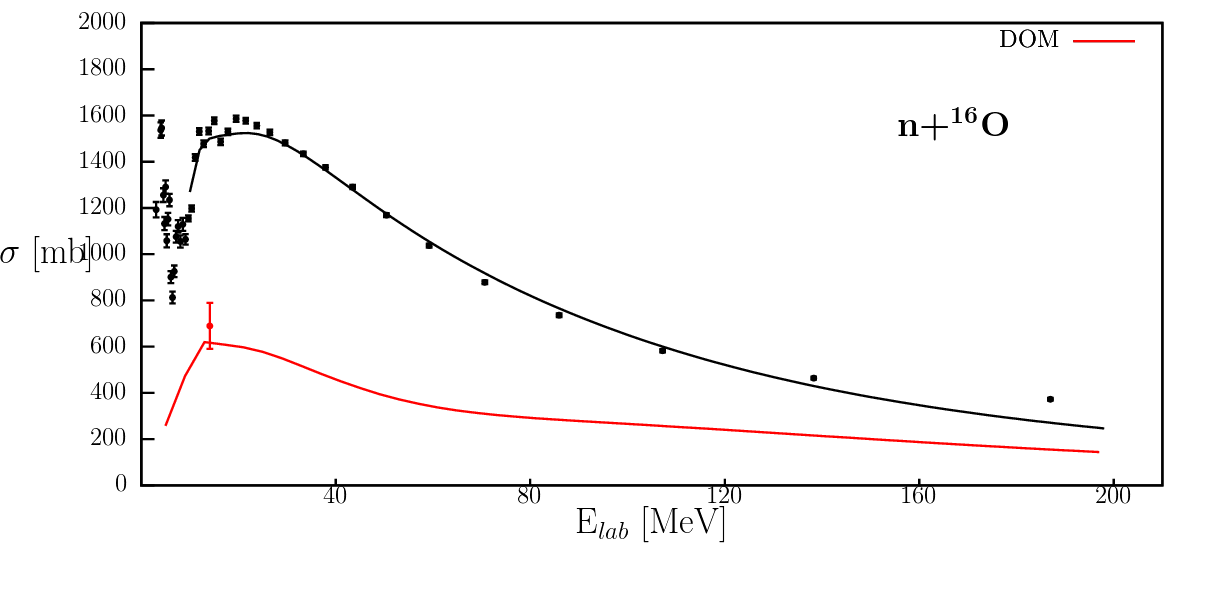
\includegraphics[width=\textwidth]{figures/o16_neutronInelastic.png}
        \label{DOM_o16_neutron_inelastic}
    \end{minipage}
    \caption{\oSix\ nucleon scattering data used in DOM fit. In all panels, experimental data
    are plotted as points and DOM calculations are shown as colored bands with
    associated one-$\sigma$ and two-$\sigma$ uncertainty regions. Panel a (c)
    shows proton (neutron) \el\ from 10-200 MeV. Panel b (d) shows proton
    (neutron) analyzing powers. Data sets are offset vertically for clarity
    and colored according to the center-of-mass scattering energy of the data
    set. Panel e shows the proton \rxn. Panel f shows the neutron \tot\ and
\rxn.}
    \label{DOM_o16_scattering}
\end{figure*}
\begin{figure*}
    \centering
    \begin{minipage}{0.45\textwidth}
        \centering
        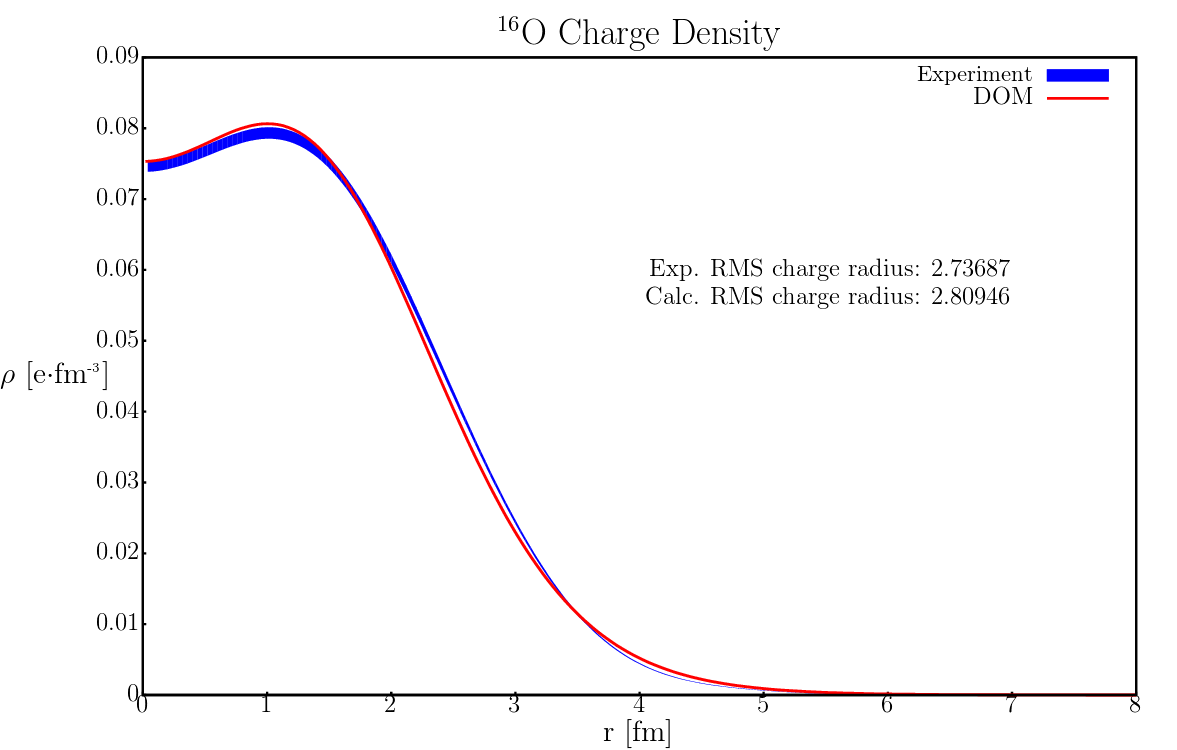
\includegraphics[width=\textwidth]{figures/o16_chargeDensity.png}
        \label{DOM_o16_chargeDensity}
    \end{minipage}
    \begin{minipage}{0.45\textwidth}
        \centering
        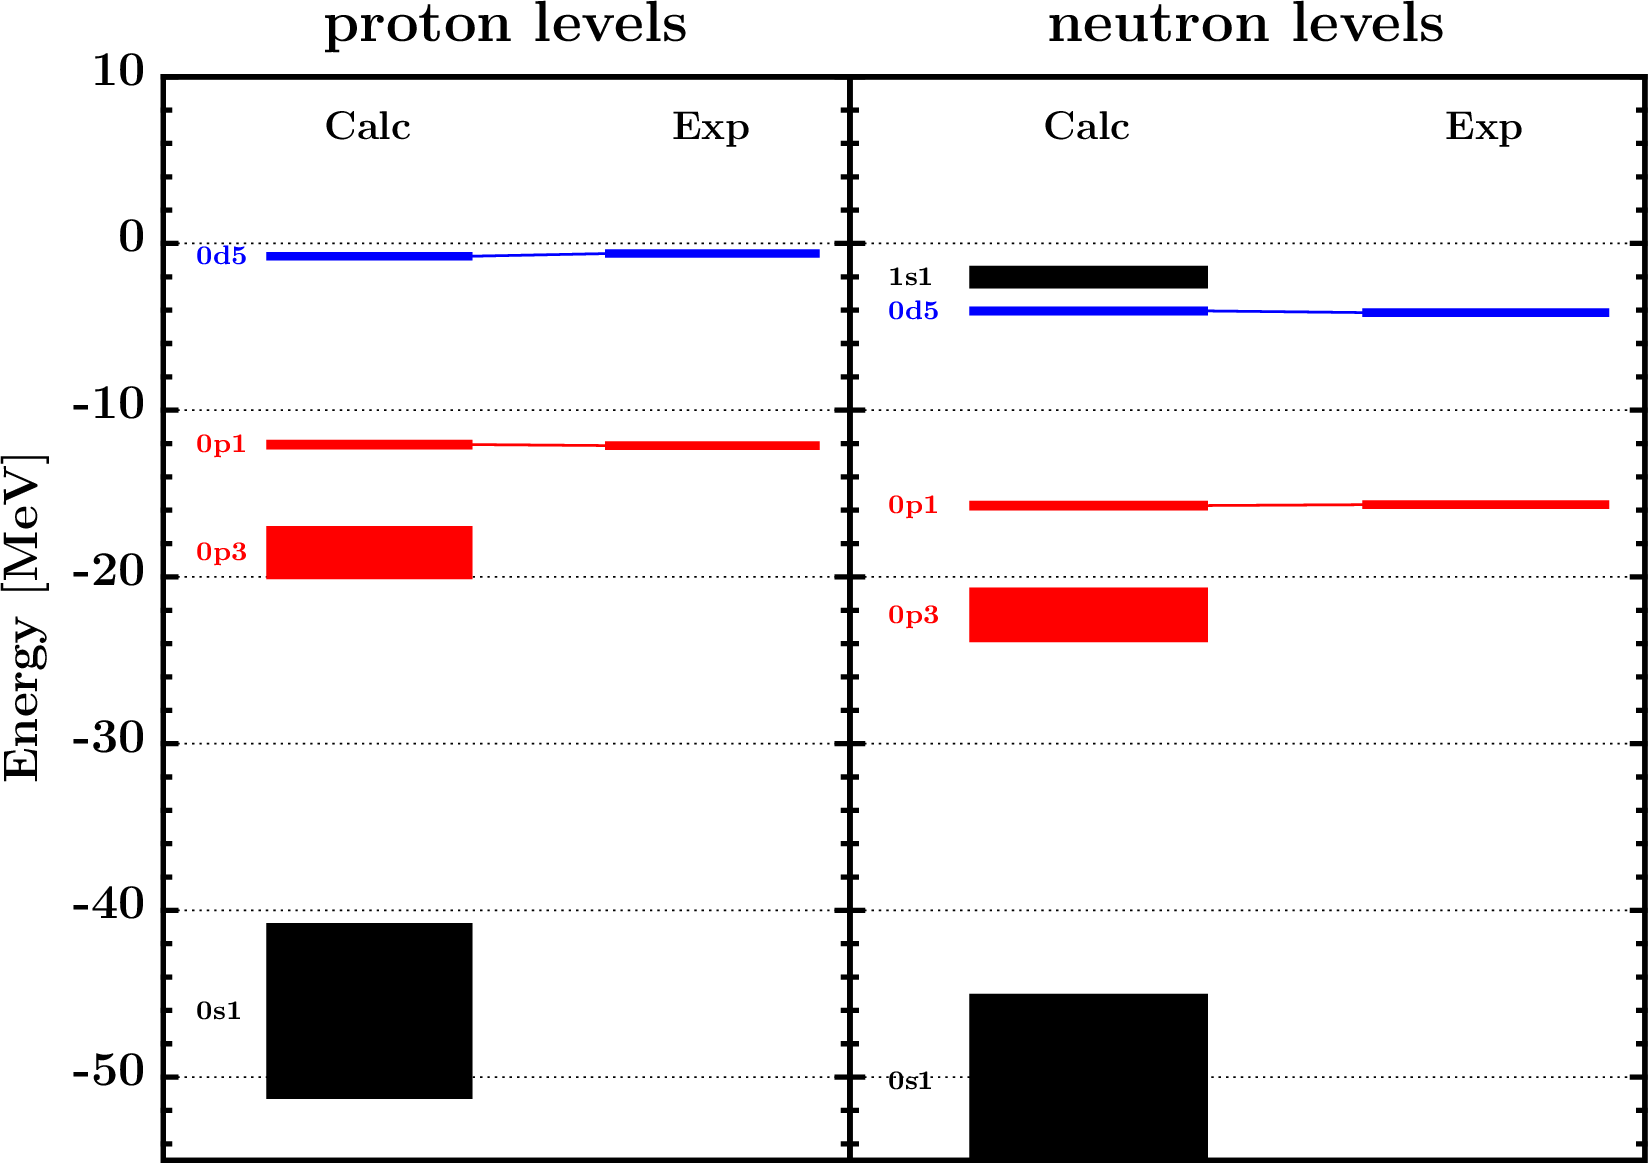
\includegraphics[width=\textwidth]{figures/o16_SPLevels.png}
        \label{DOM_o16_SPLevels}
    \end{minipage}
    \begin{minipage}{0.45\textwidth}
        \centering
        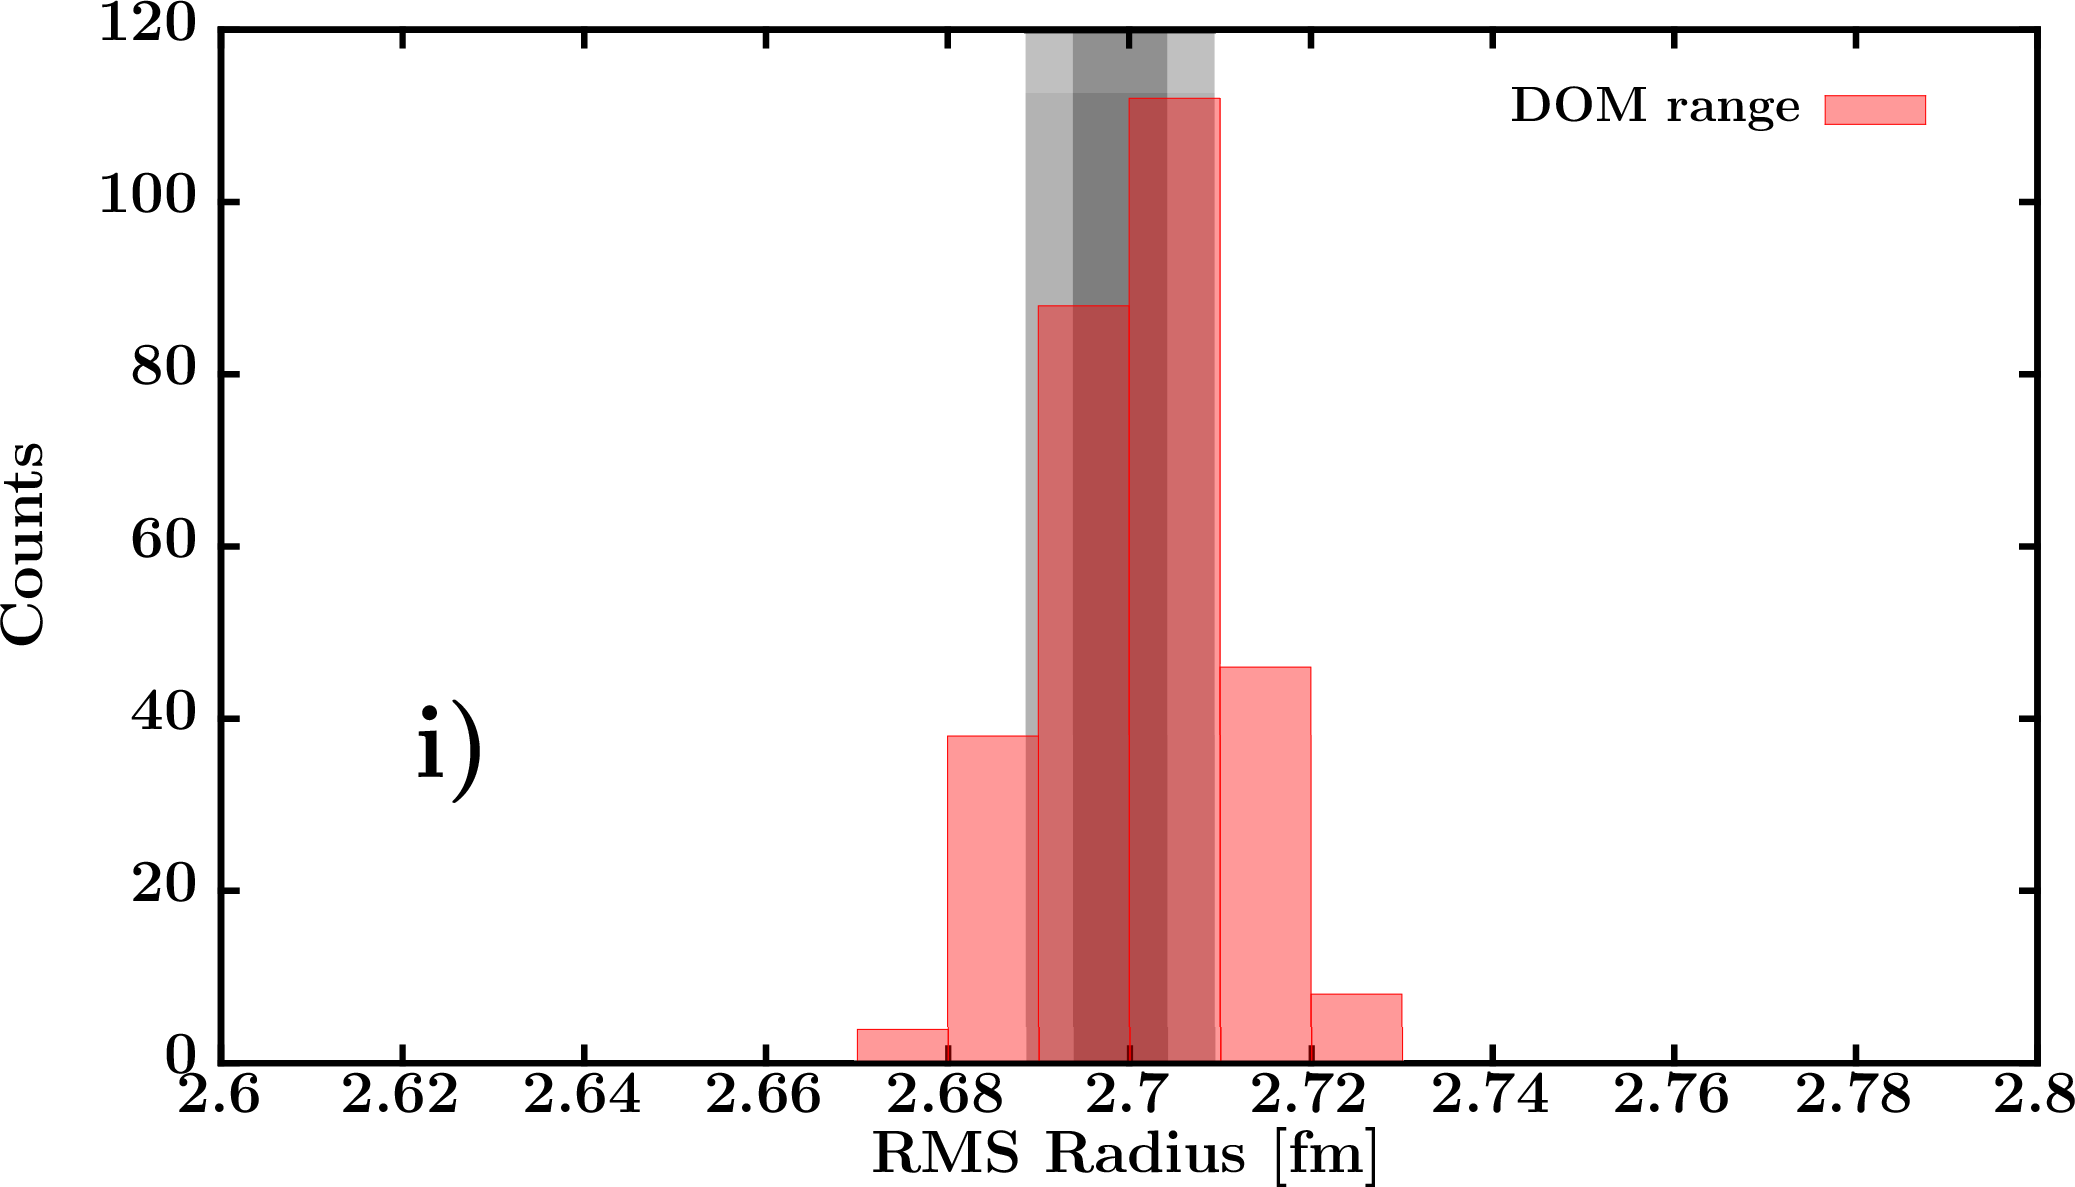
\includegraphics[width=\textwidth]{figures/o16_RMSRadius.png}
        \label{DOM_o16_RMSRadius}
    \end{minipage}
    \begin{minipage}{0.45\textwidth}
        \centering
        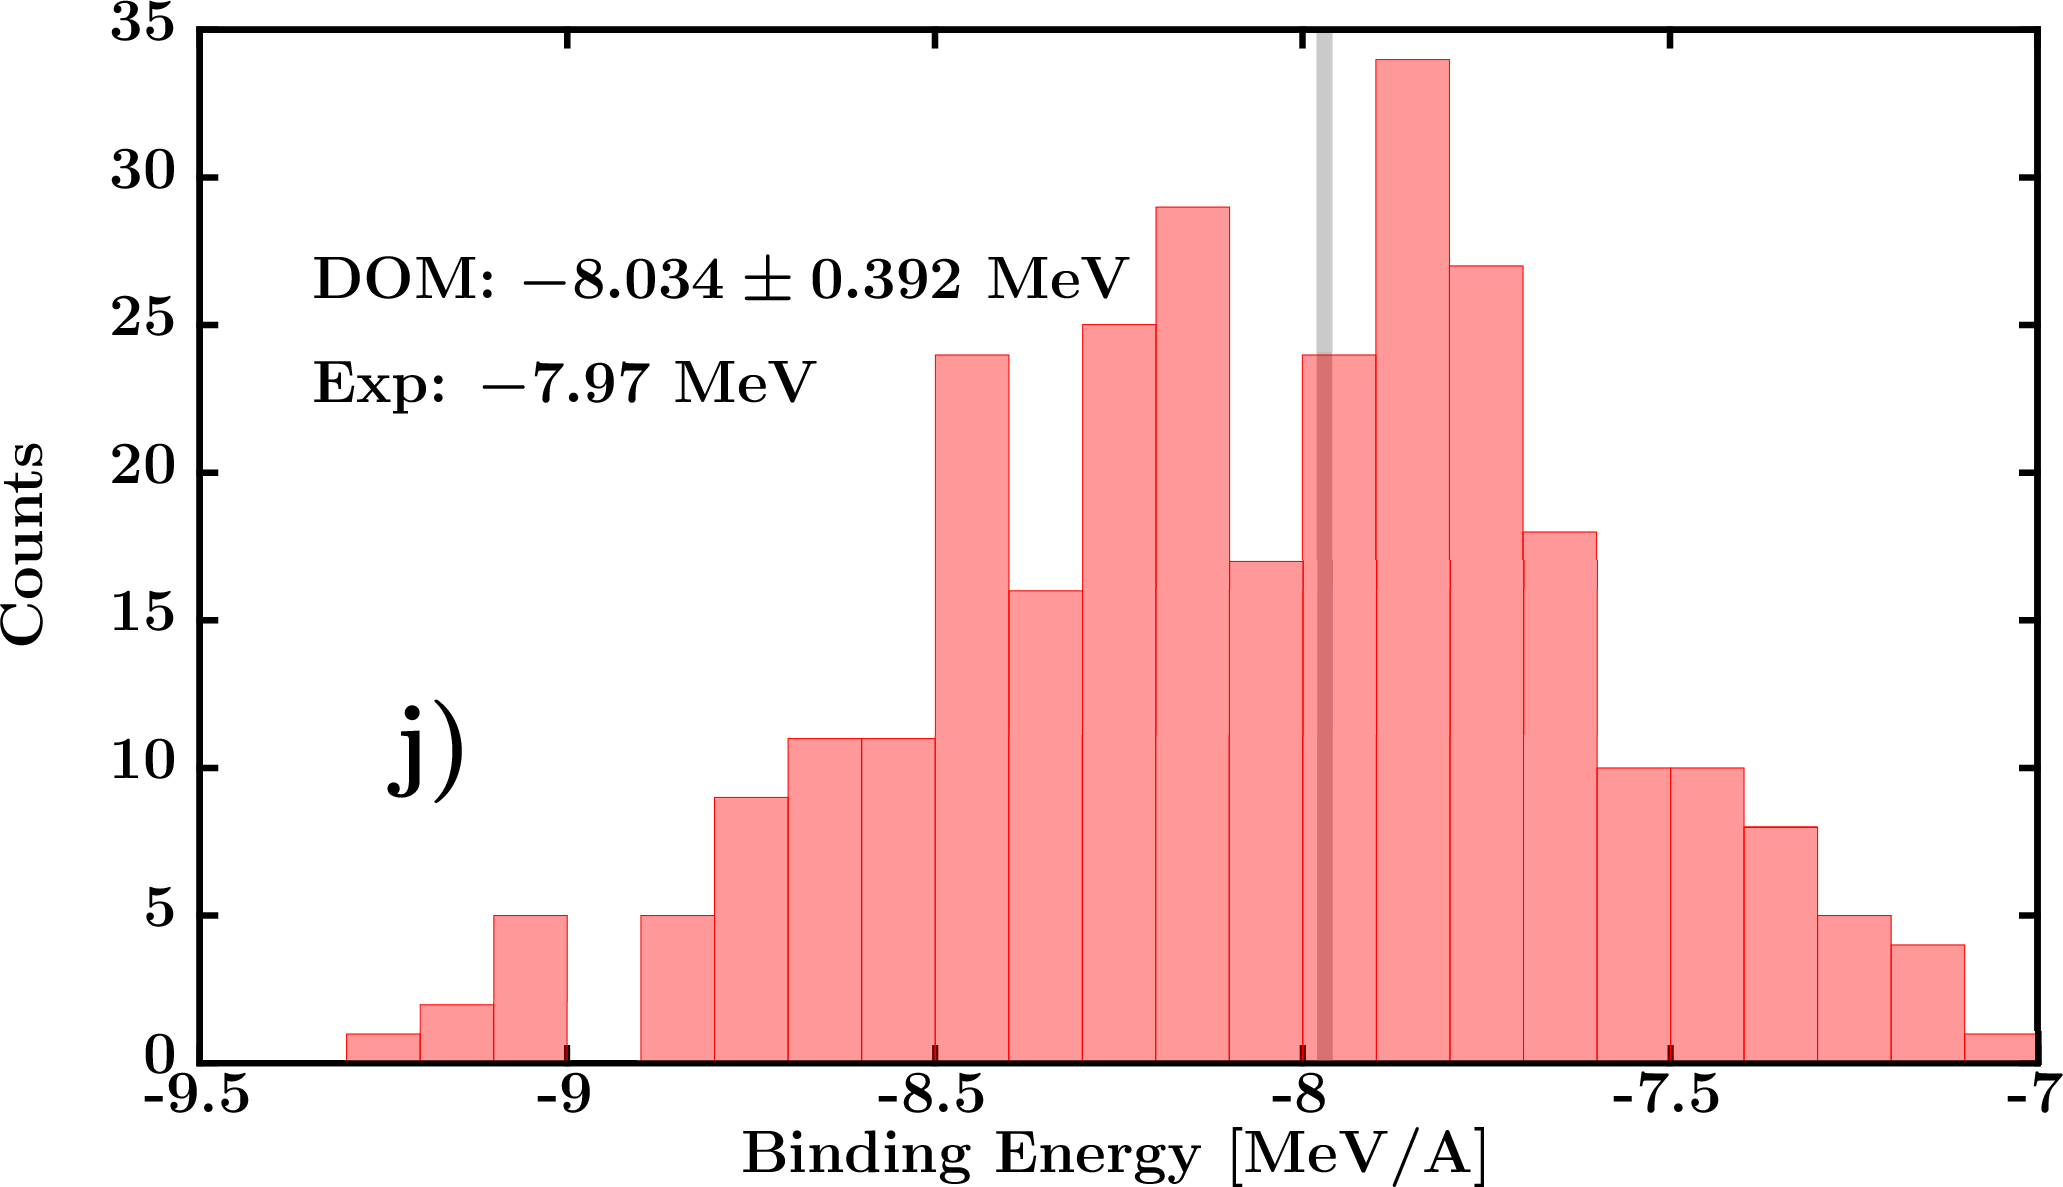
\includegraphics[width=\textwidth]{figures/o16_BE.png}
        \label{DOM_o16_BE}
    \end{minipage}
    \caption{\oSix\ structural data used in DOM fit. Panel a shows the charge
        density distribution: the ``experimental'' data of \cite{DeVries1987}
        are shown with an arbitrary 1\% error band and the DOM calculation is
        shown with associated one-$\sigma$ and two-$\sigma$ uncertainty regions.
        Panel b shows the DOM-calculated single-particle energies for protons
        and neutrons with a one-sigma error band (left side of each subpanel) and
        the known neutron and proton valence level energies, from \cite{AME2016}.
        Panels c and d show the DOM-calculated RMS charge radius and binding energy per
    nucleon, respectively; experimental values/uncertainties are shown in gray.}
    \label{DOM_o16_structural}
\end{figure*}

Figs. \ref{DOM_o16_scattering} and \ref{DOM_o16_structural} show the
DOM fit of \oSix\ to the experimental data used to constrain the potential via
MCMC sampling.  The experimental proton \rxn\, neutron \el, \tot, 
and \rxn\, charge density distribution, RMS charge radius, binding energy per nucleon,
and \pOne\ and \dFive\ single-particle energy data are all well-reproduced,
suggesting that the DOM is a robust modeling tool for nuclei as light as A=16.
Almost all experimental proton \el\ data are recovered by the DOM
calculations with the exception of the location and magnitude of the diffraction
minima at backward angles, a failure common to many past optical model analyses.
The assumption that the DOM optical potential can be factored into
independent radial and energy-dependent terms may be responsible for the poorer
performance of the DOM in this region.

The analyzing powers appear to be the most difficult sector of experimental data to
reproduce, with moderate deviations visible from 10-15 MeV for both protons and
neutrons and above 100 MeV for
protons (see panels B and D of Fig. \ref{DOM_o16_scattering}). Some
of the difficulty with the analyzing powers is attributable to our neglecting of
an imaginary spin-orbit term in the DOM potential used in this work, a choice
made due to the unreasonable unbounded growth of the imaginary spin-orbit term
as $\ell$ grows in the traditional $\ell\cdot\sigma$ definition used in
\cite{KoningDelaroche}. Future DOM analyses may demand a more sophisticated spin-orbit treatment.

\textcolor{red}{comments on pseudo-data for reaction cross section; relative value of TCS, ECS, and RCS data; importance of charge density distribution.}

\subsection{Fit results on $^{18}$O}
\begin{figure*}[!htb]
    \centering
    \begin{minipage}{0.45\textwidth}
        \centering
        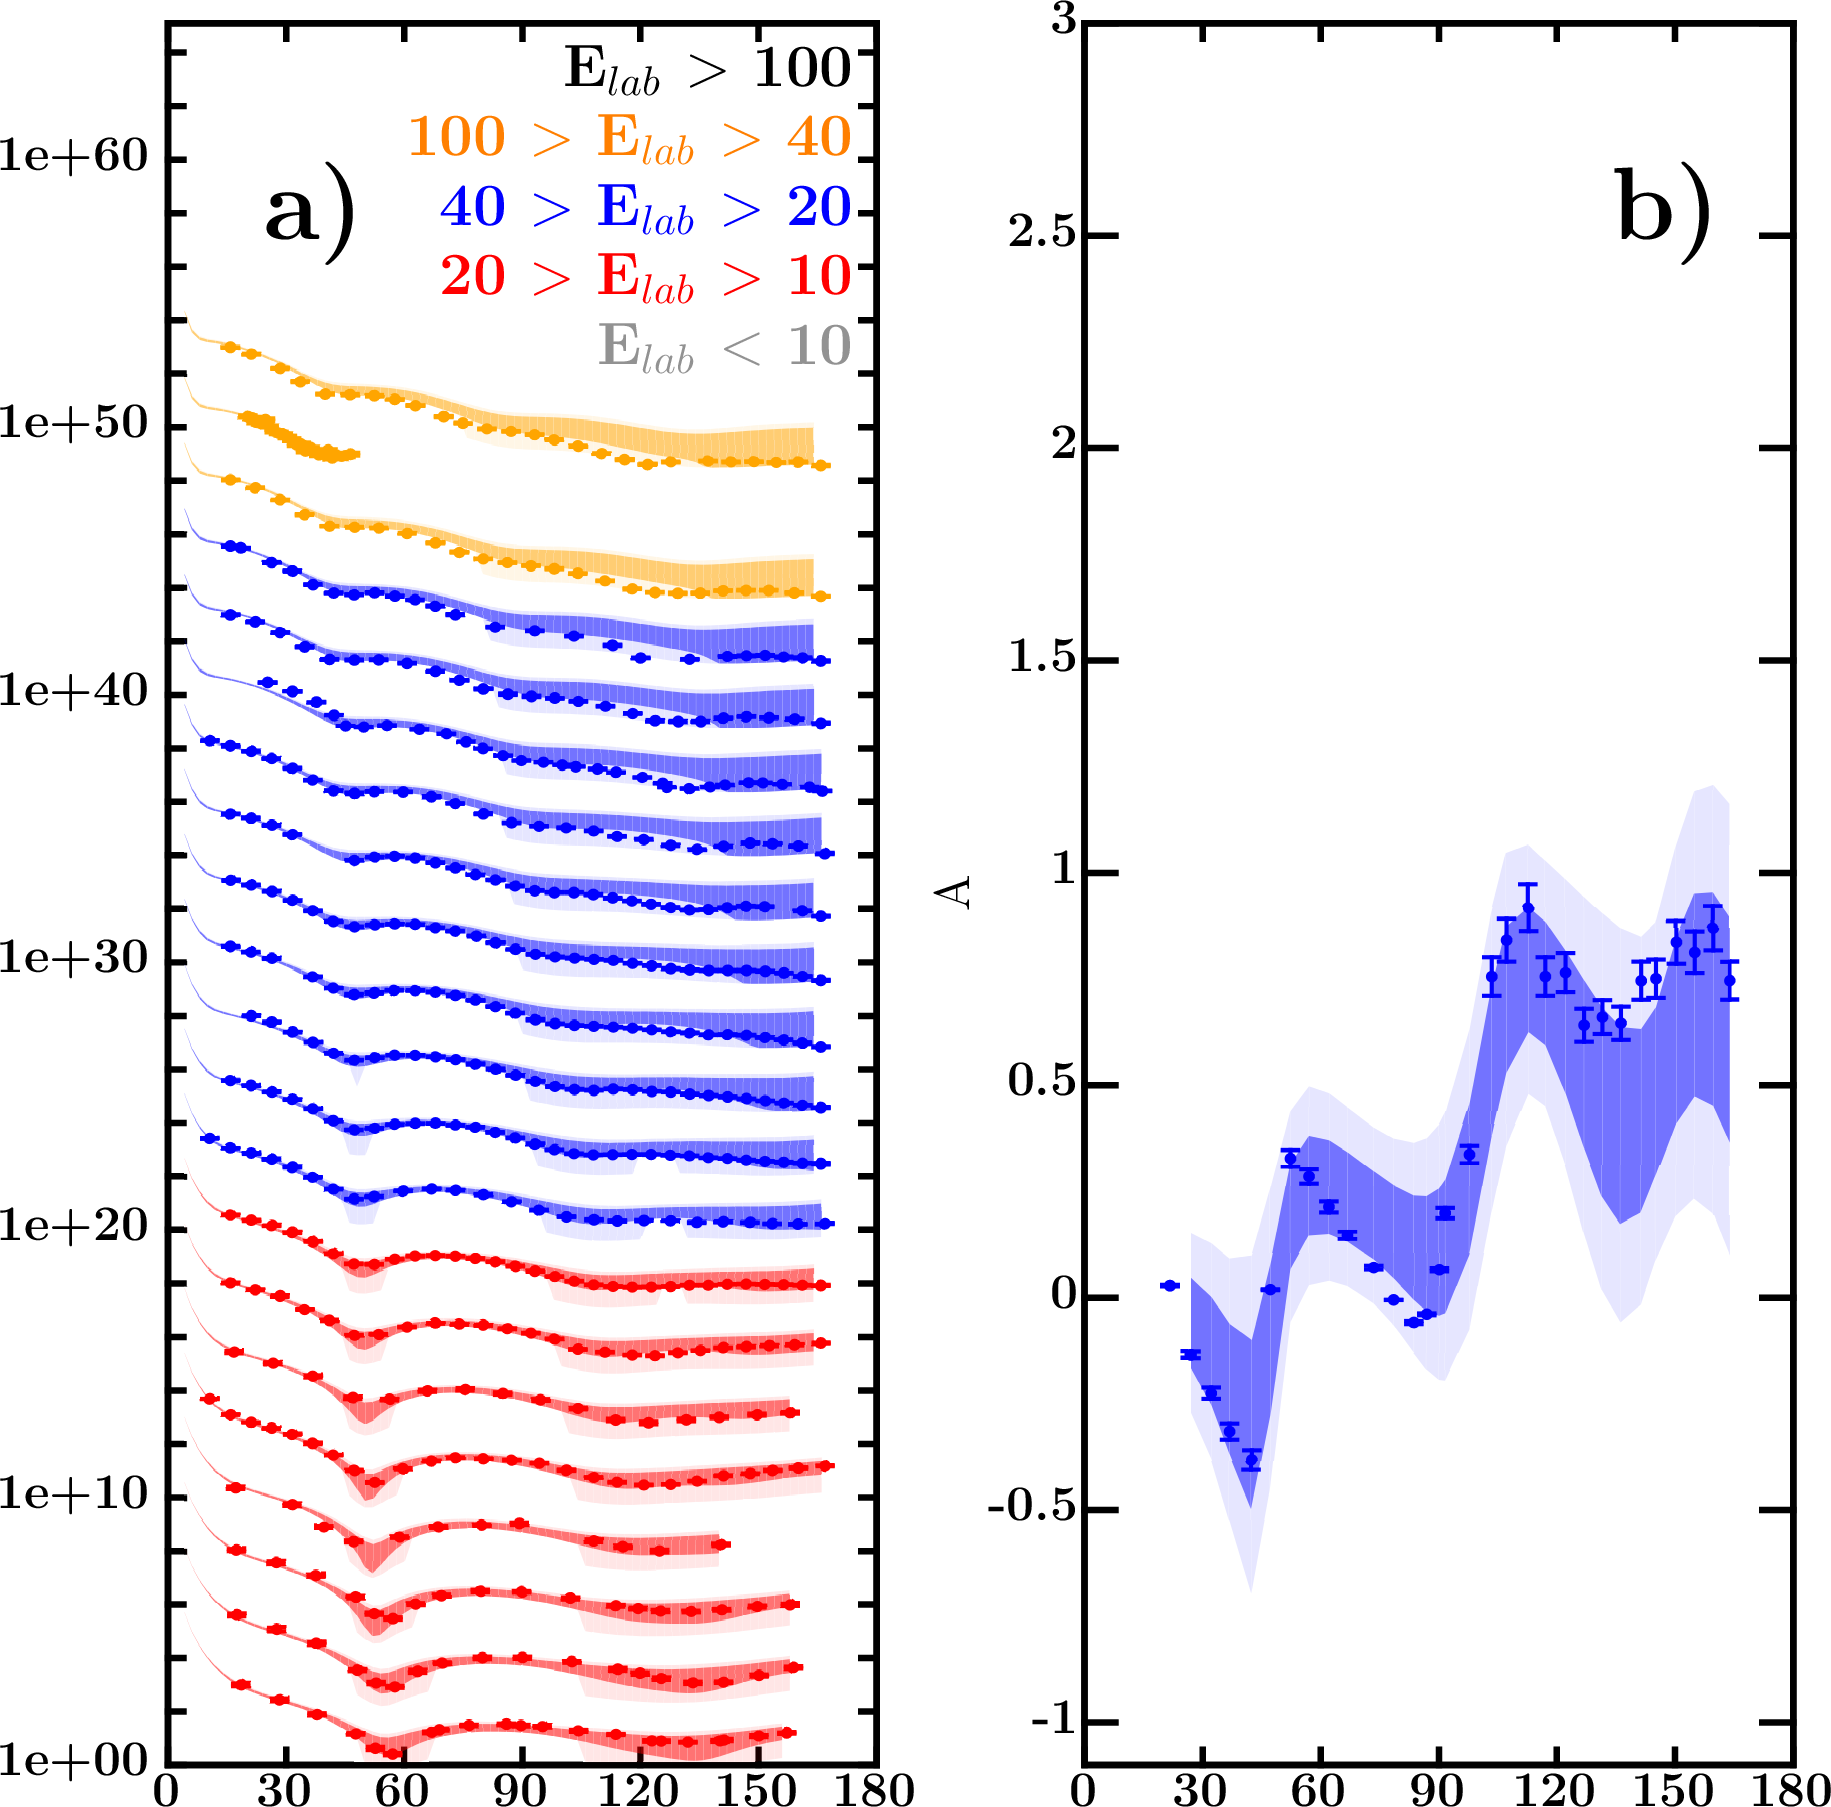
\includegraphics[width=\textwidth]{figures/o18_protonElastic.png}
        \label{DOM_o18_proton_elastic}
    \end{minipage}\hspace{6pt}
    \begin{minipage}{0.45\textwidth}
        \centering
        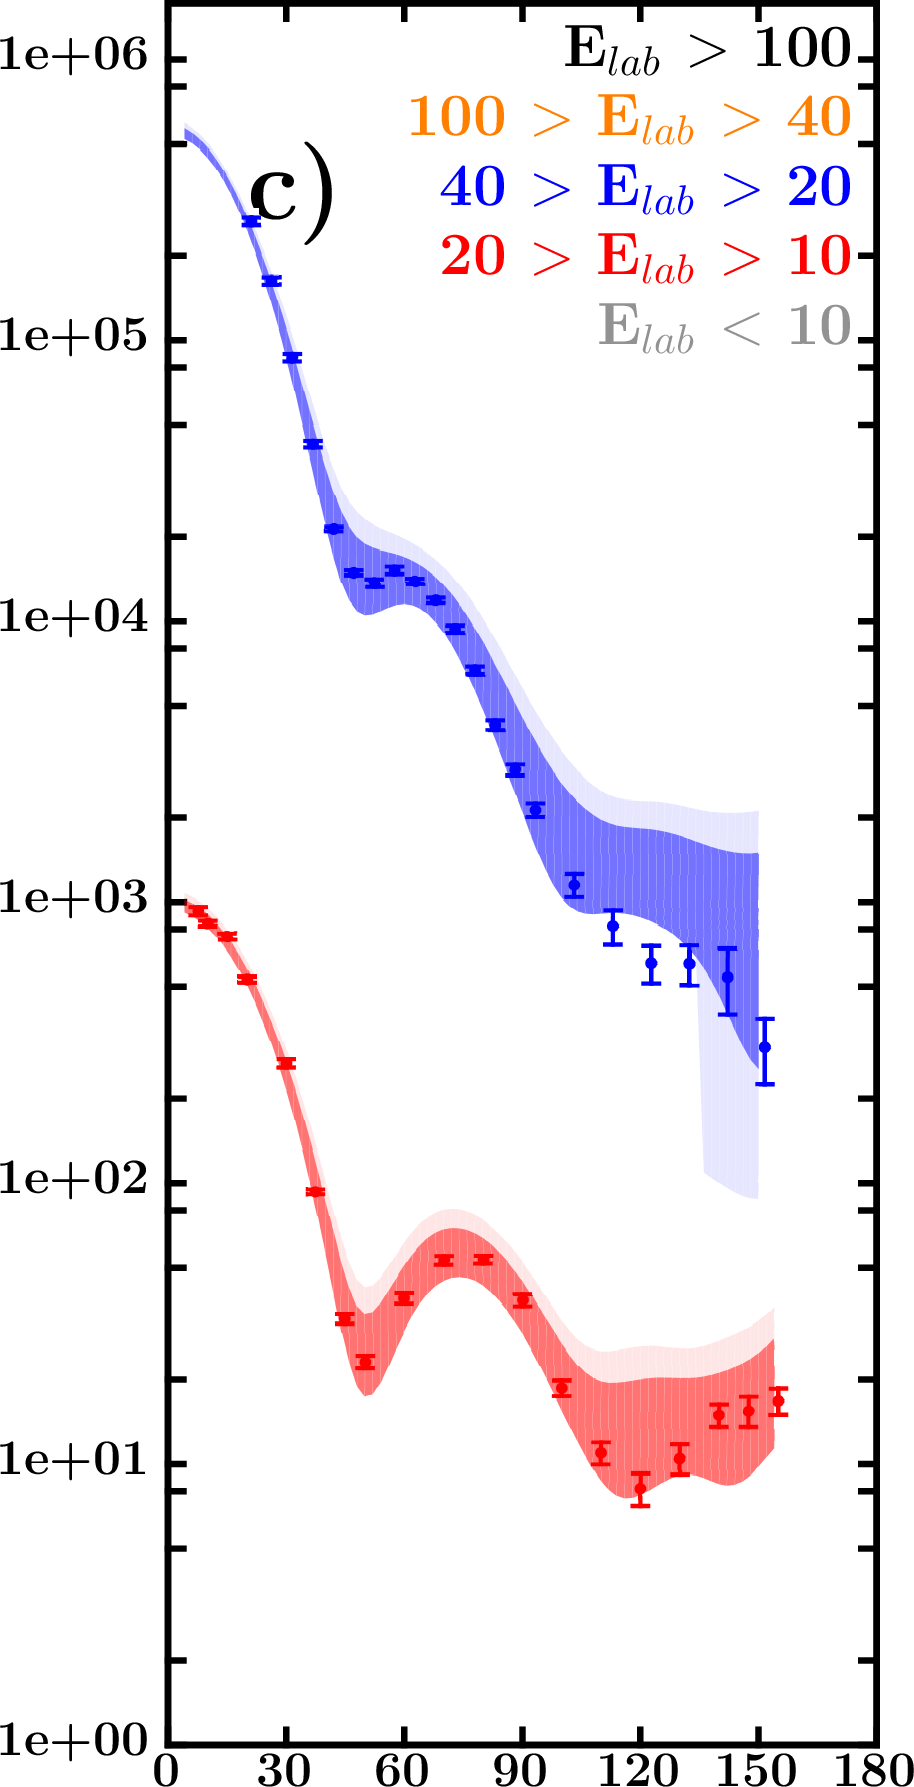
\includegraphics[width=\textwidth]{figures/o18_neutronElastic.png}
        \label{DOM_o18_neutron_elastic}
    \end{minipage}
    \centering
    \begin{minipage}{0.45\textwidth}
        \centering
        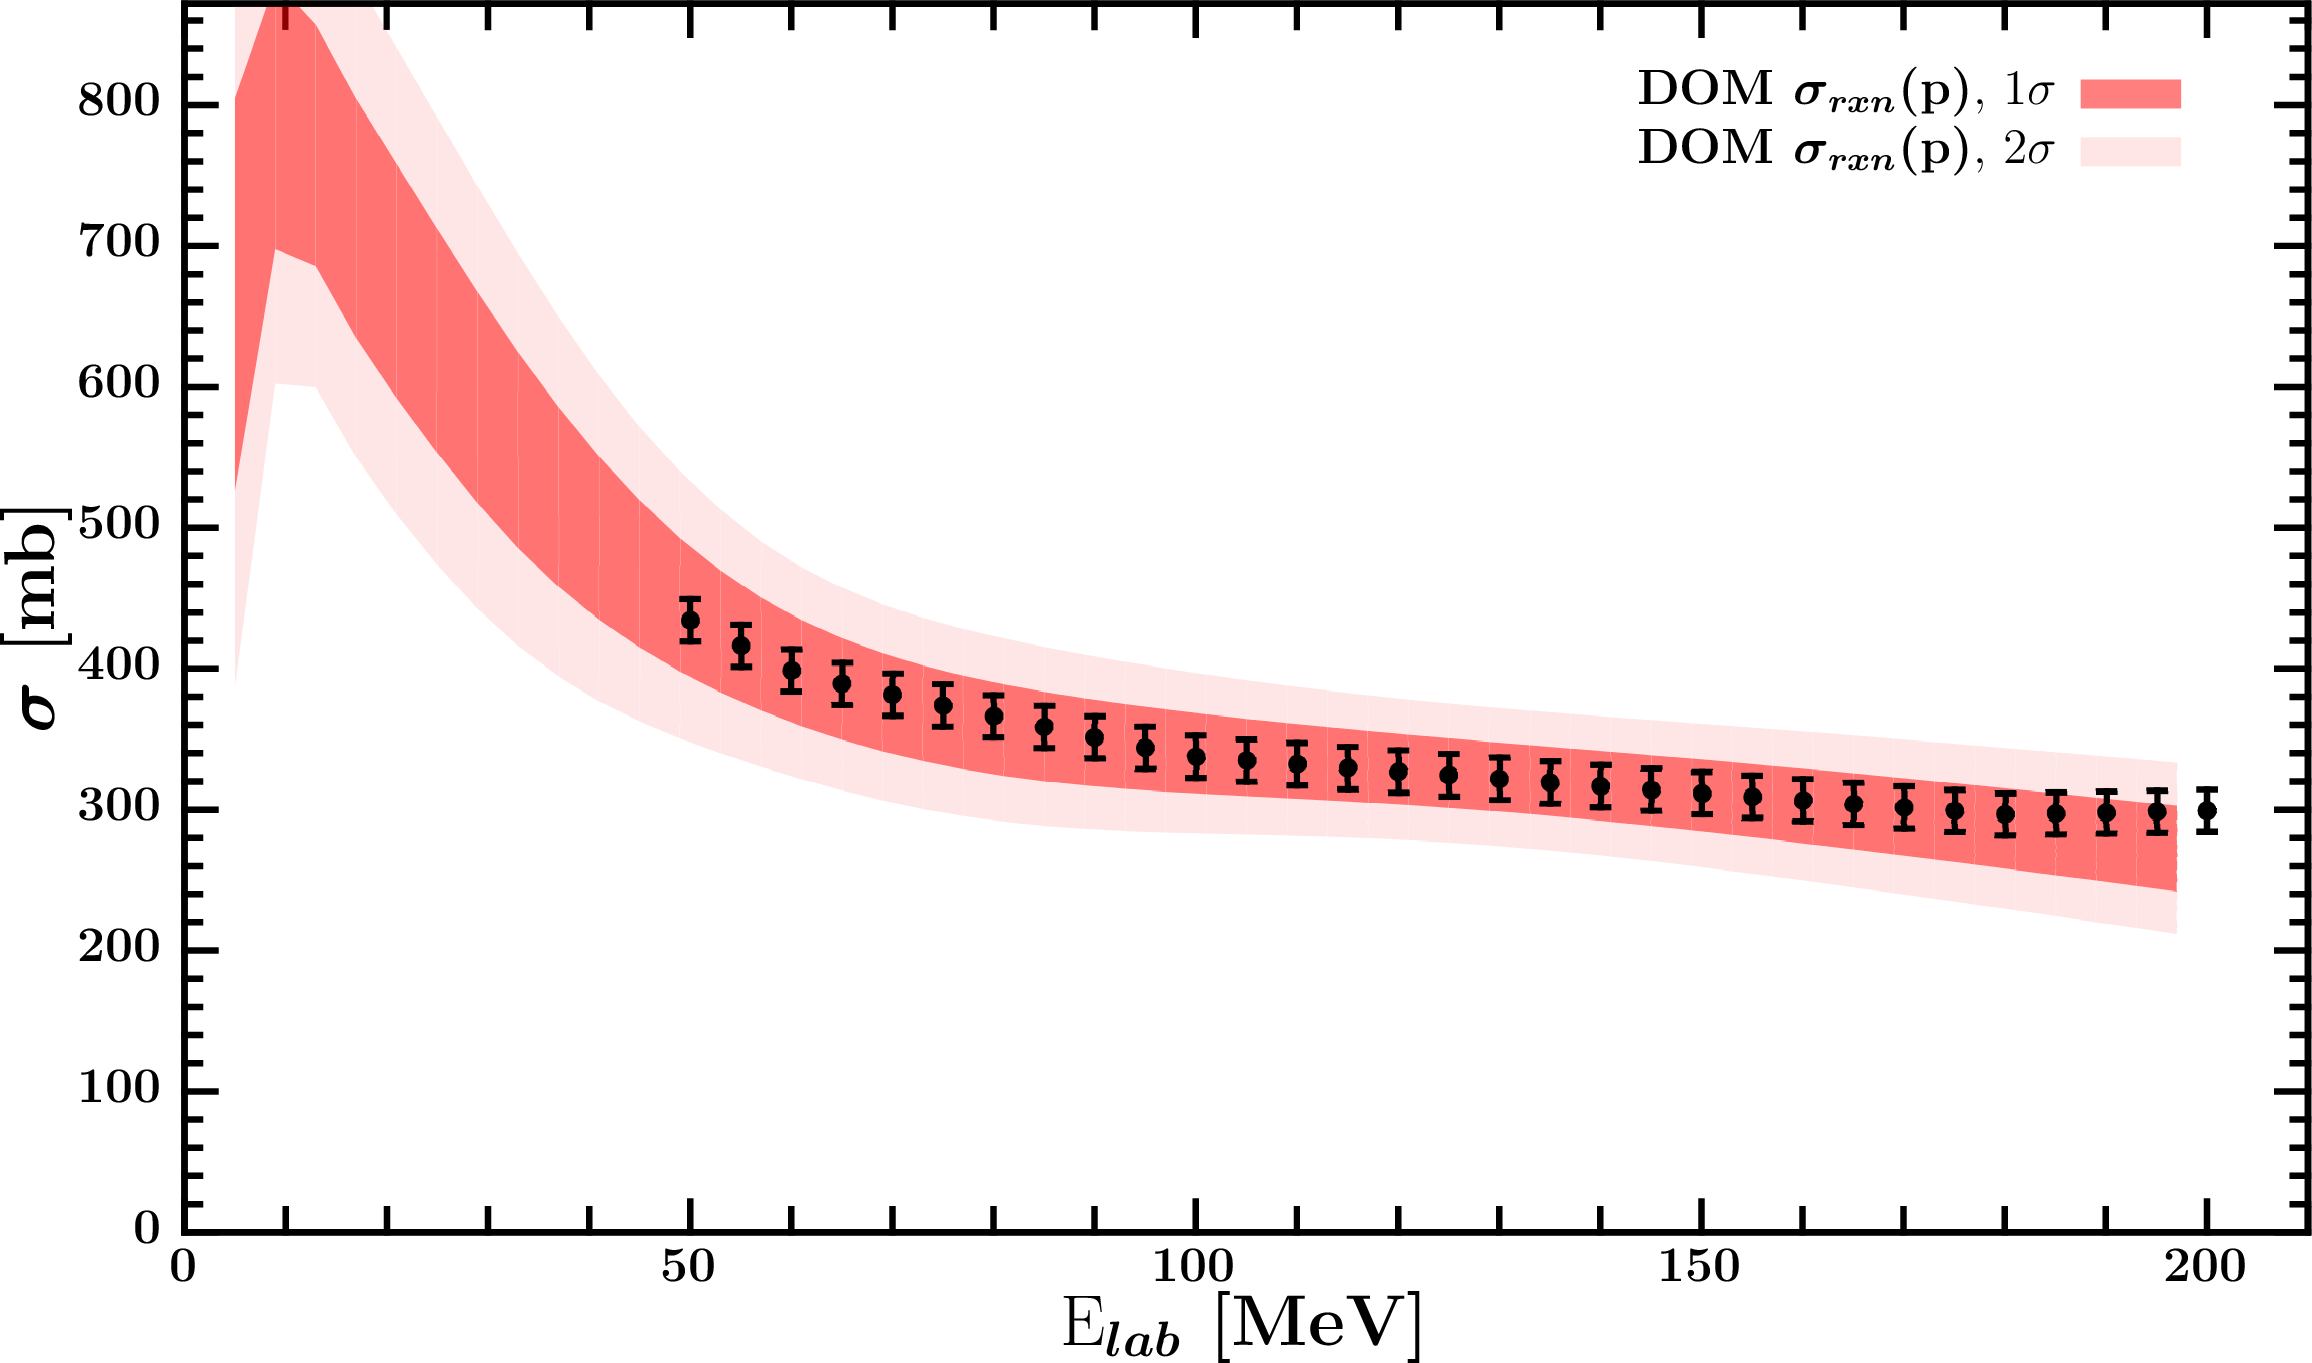
\includegraphics[width=\textwidth]{figures/o18_protonInelastic.png}
        \label{DOM_o18_proton_inelastic}
    \end{minipage}\hspace{6pt}
    \begin{minipage}{0.45\textwidth}
        \centering
        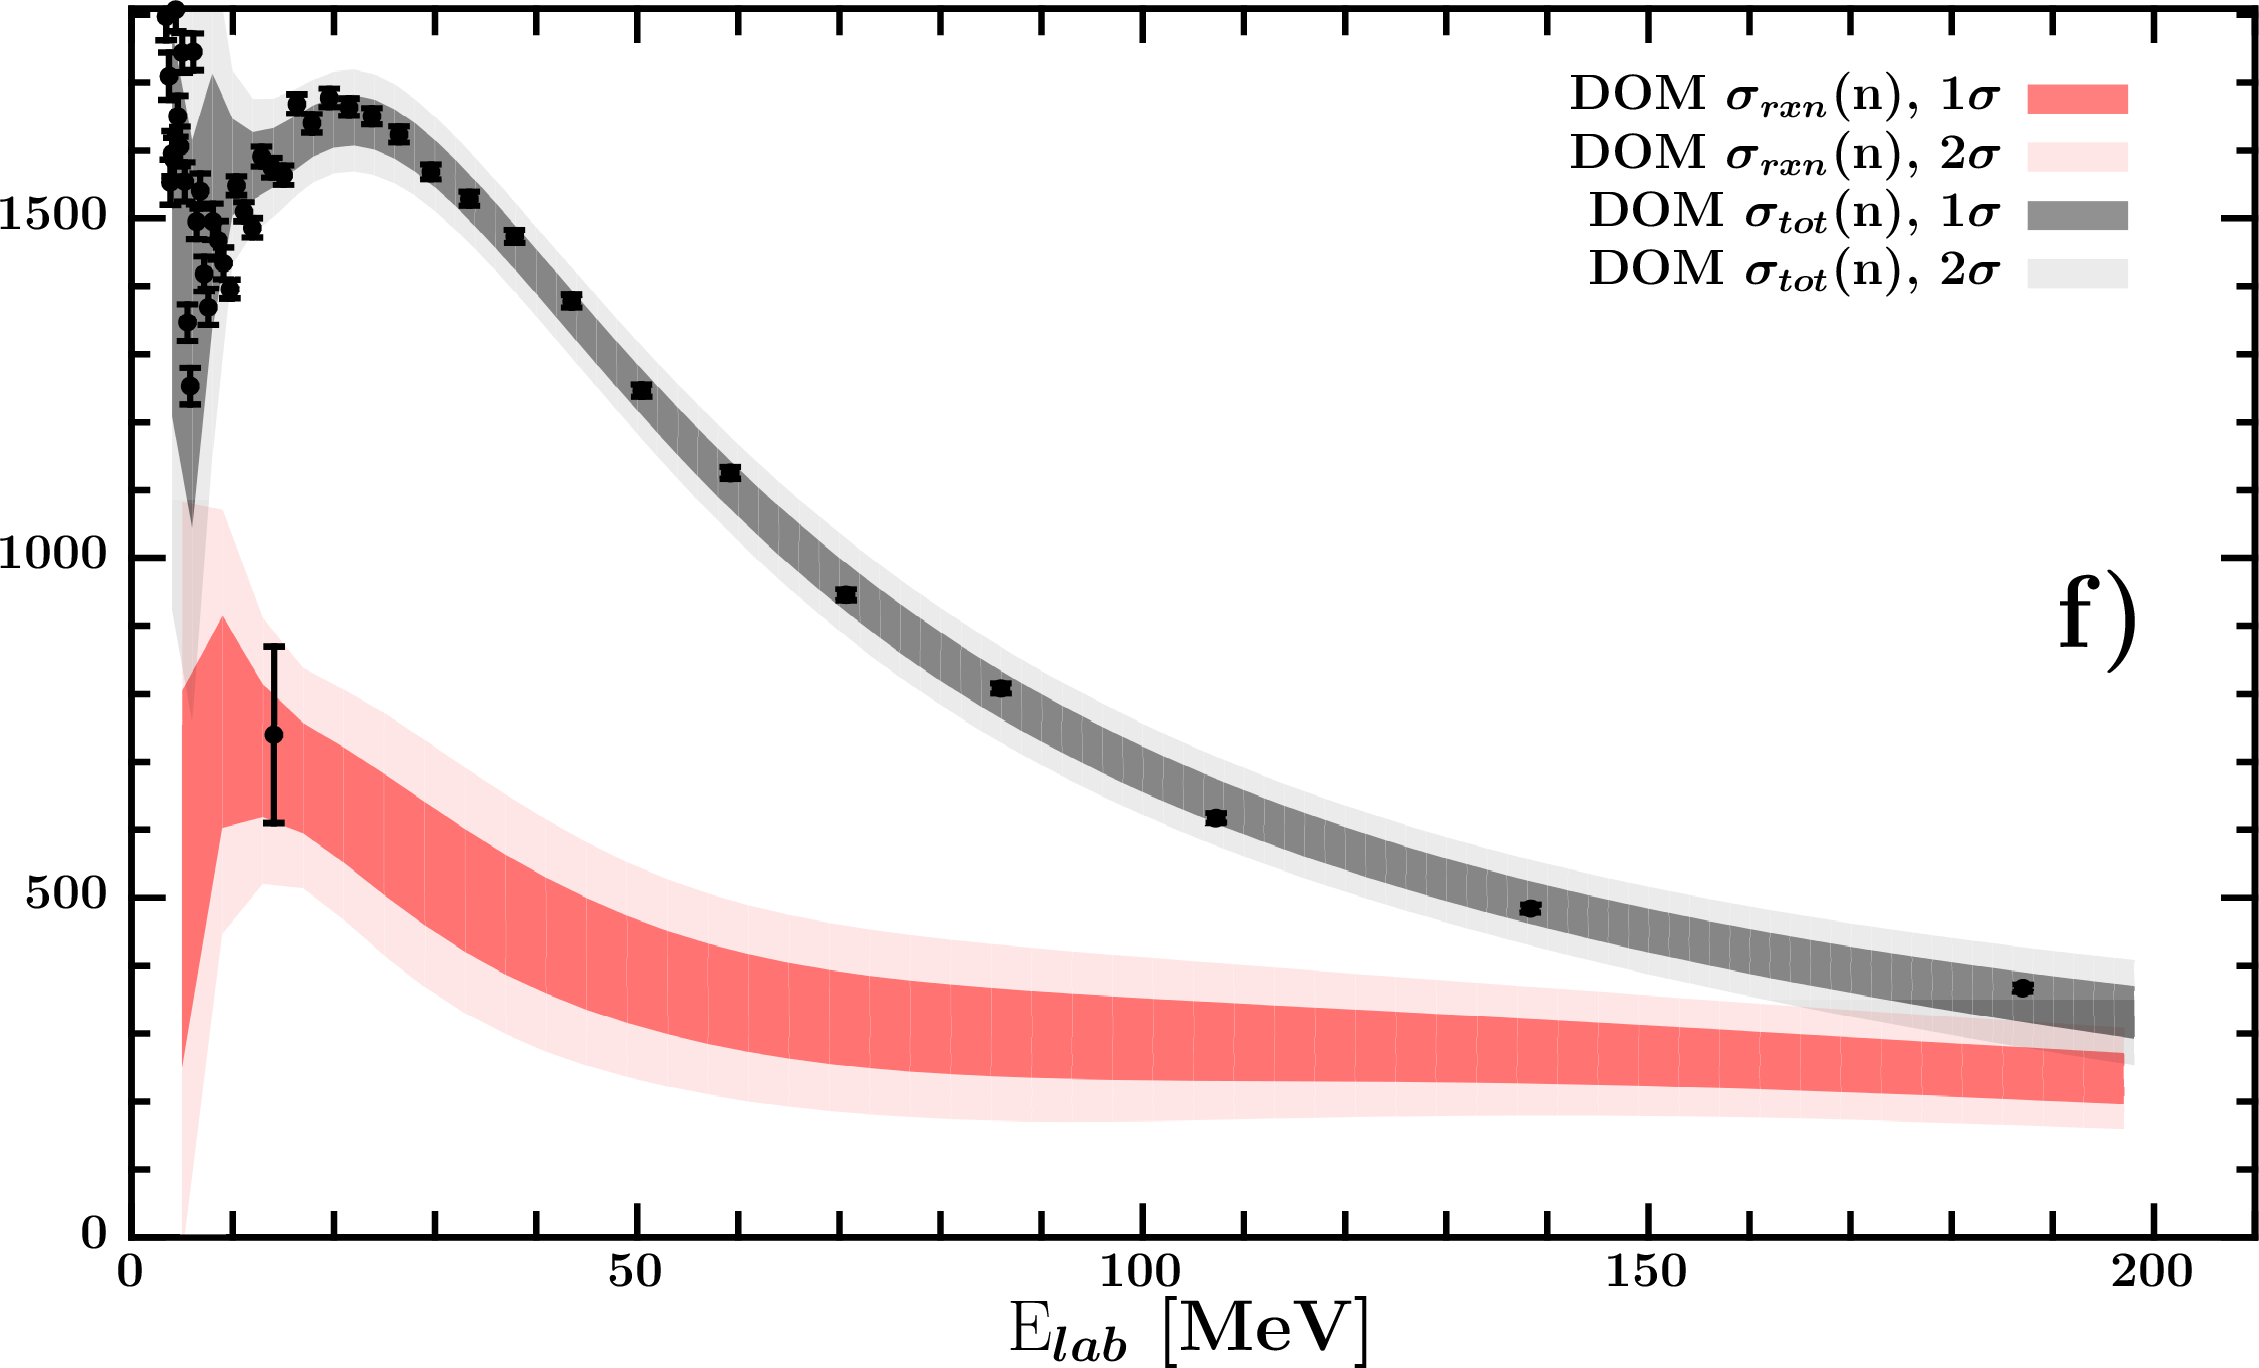
\includegraphics[width=\textwidth]{figures/o18_neutronInelastic.png}
        \label{DOM_o18_neutron_inelastic}
    \end{minipage}
    \caption{\oEight\ nucleon scattering data used in DOM fit. In all panels, experimental data
    are plotted as points and DOM calculations are shown as colored regions with
    associated one-$\sigma$ and two-$\sigma$ uncertainty bands. Panel a (c)
    shows proton (neutron) \el\ from 10-200 MeV. Panel b (d) shows proton
    (neutron) analyzing powers. Data sets are offset vertically for clarity
    and colored according to the center-of-mass scattering energy of the data
    set. Panel e shows the proton \rxn. Panel f shows the neutron \tot\ and
\rxn.}
    \label{DOM_o18_scattering}
\end{figure*}
\begin{figure*}
    \centering
    \begin{minipage}{0.45\textwidth}
        \centering
        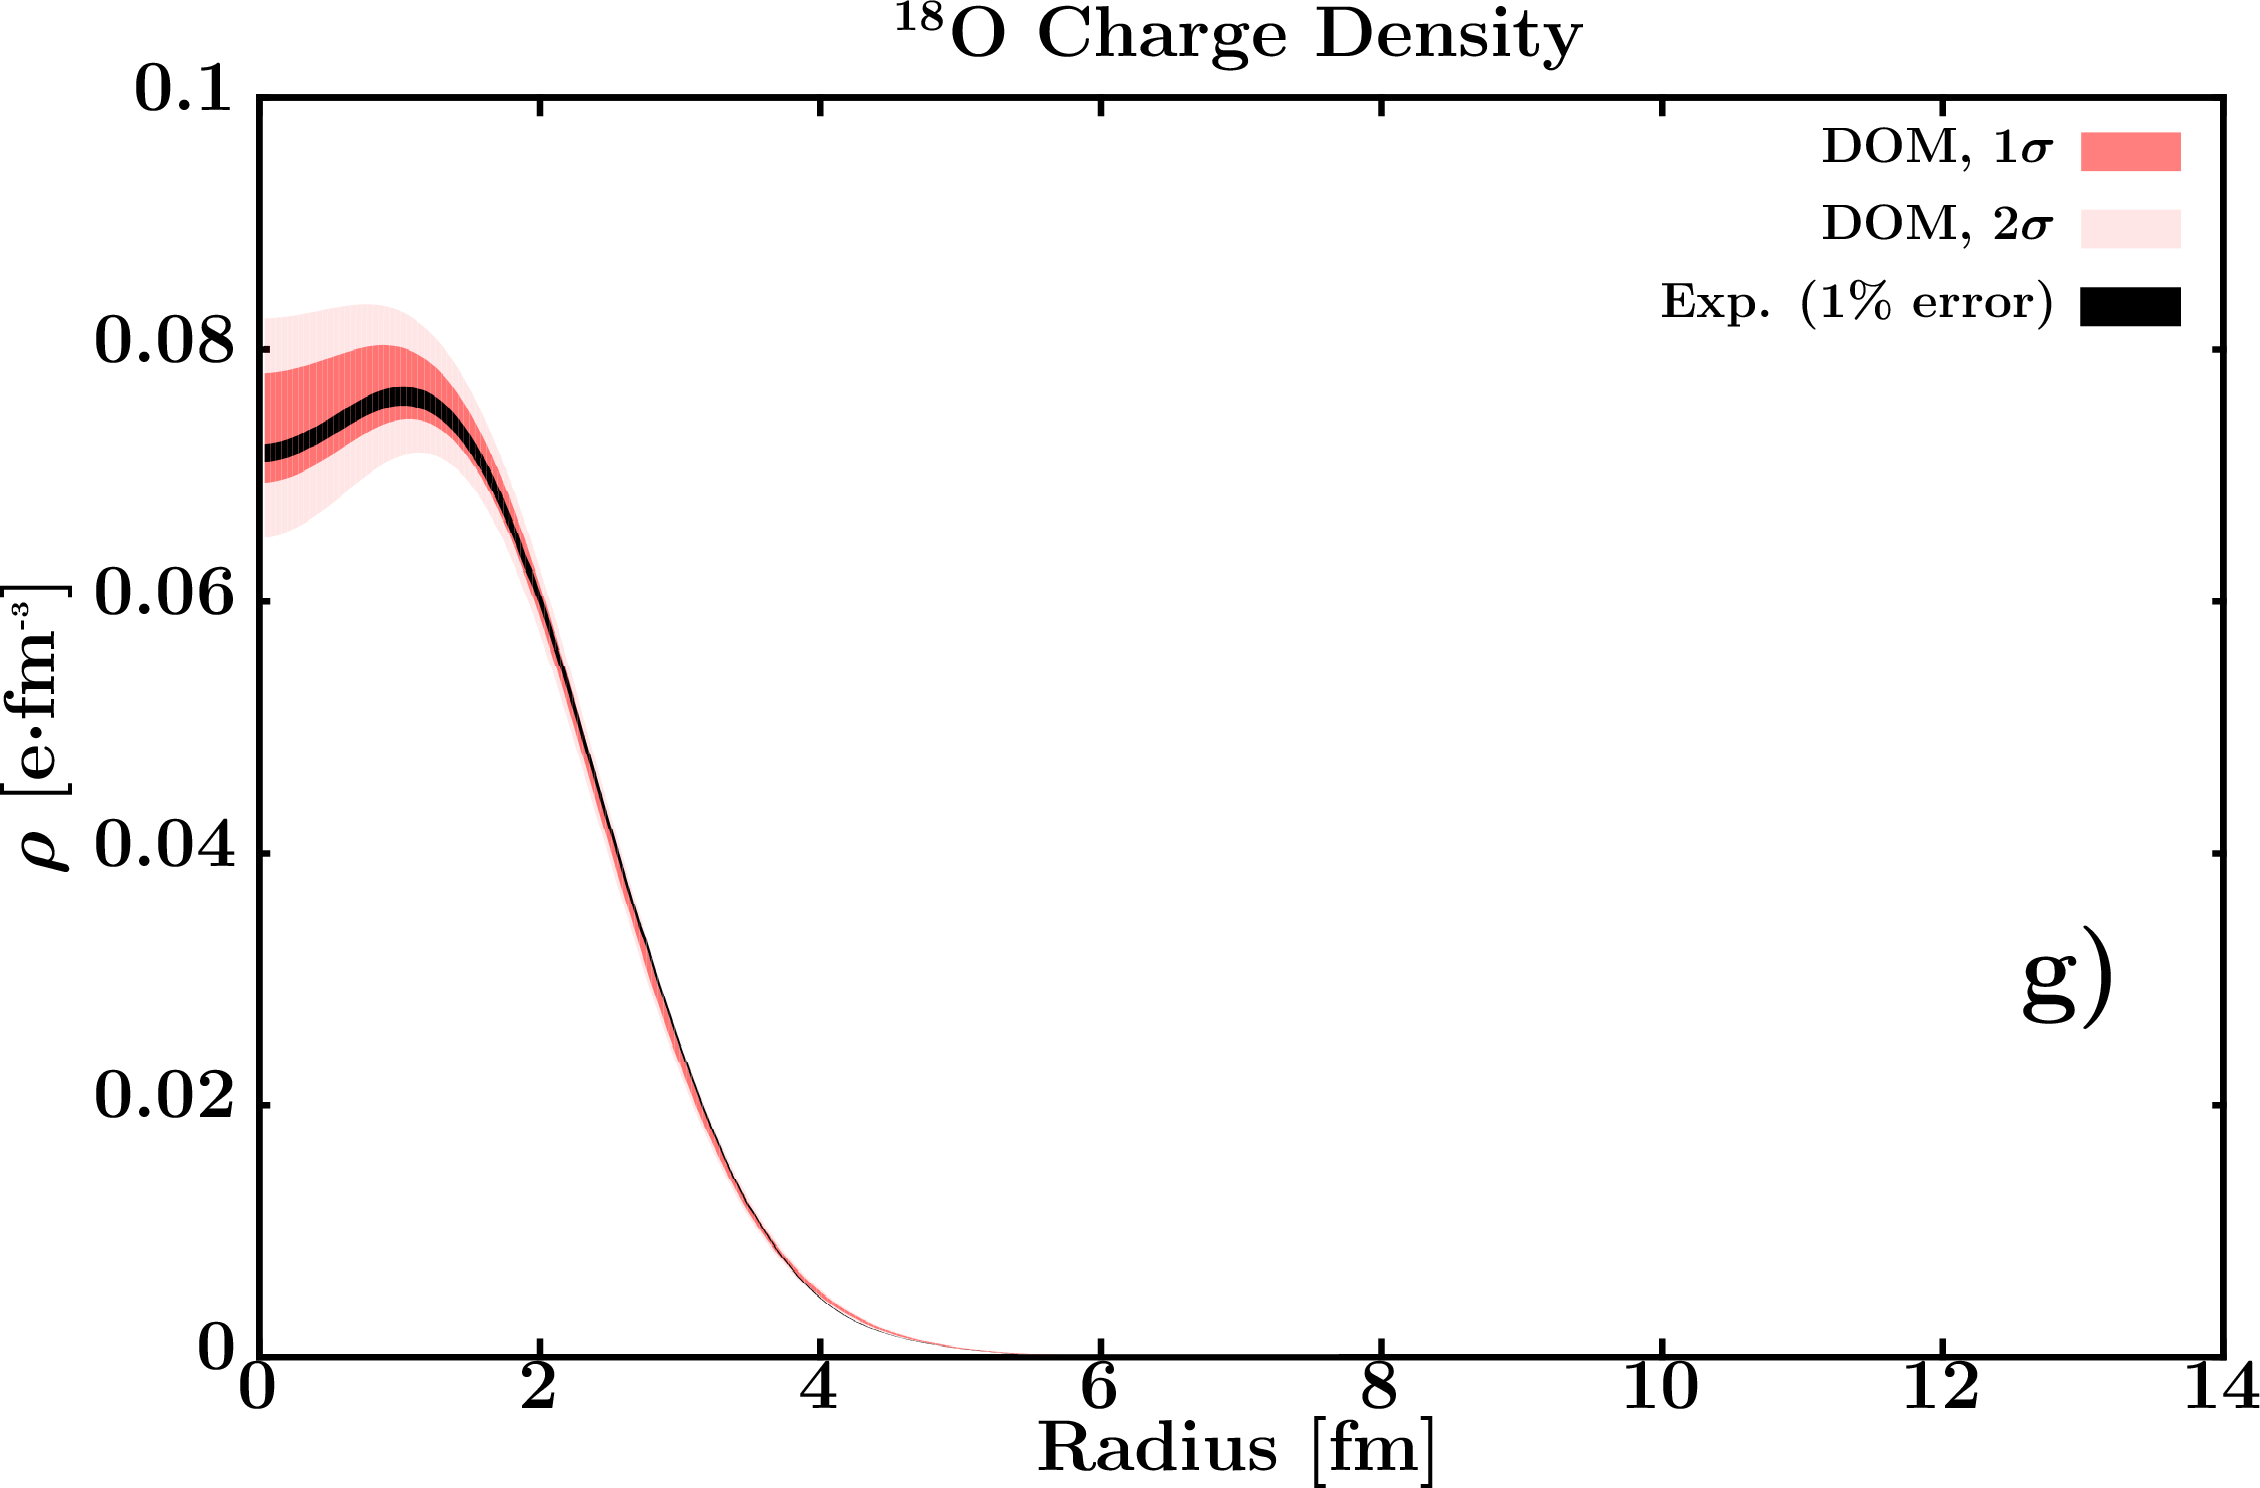
\includegraphics[width=\textwidth]{figures/o18_chargeDensity.png}
        \label{DOM_o18_chargeDensity}
    \end{minipage}
    \begin{minipage}{0.45\textwidth}
        \centering
        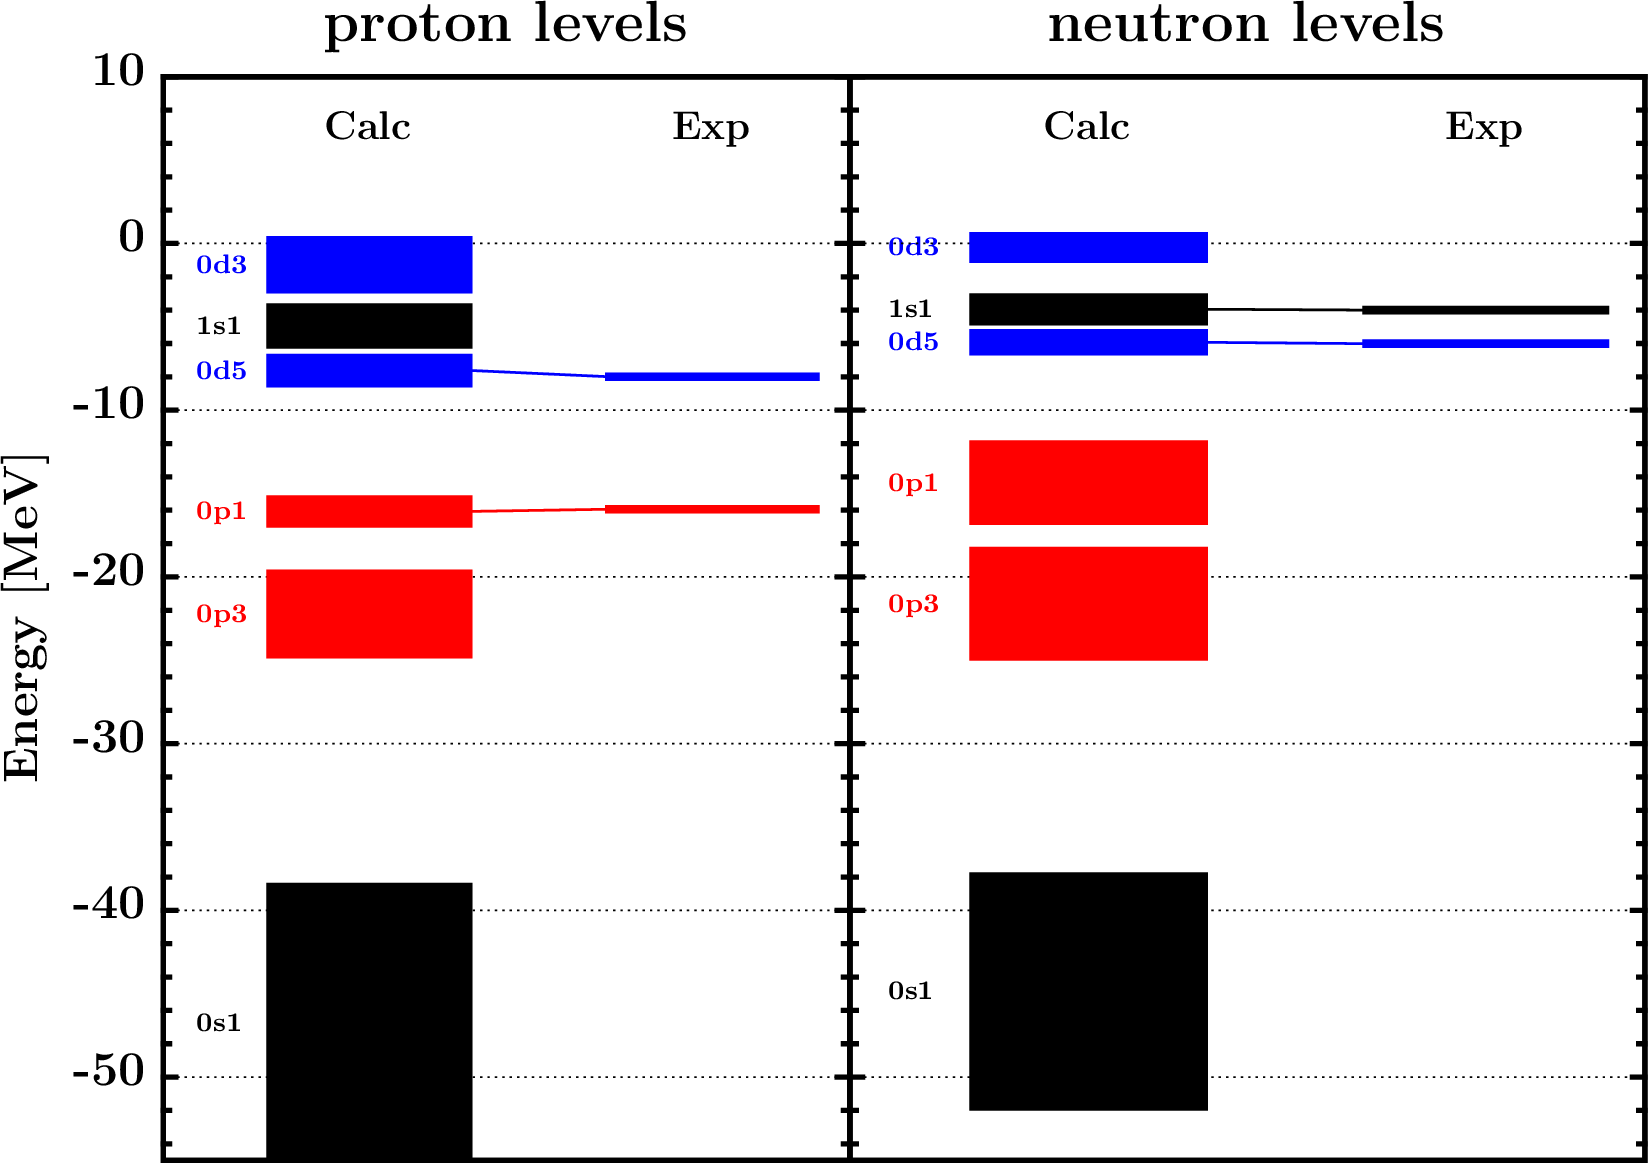
\includegraphics[width=\textwidth]{figures/o18_SPLevels.png}
        \label{DOM_o18_SPLevels}
    \end{minipage}
    \begin{minipage}{0.45\textwidth}
        \centering
        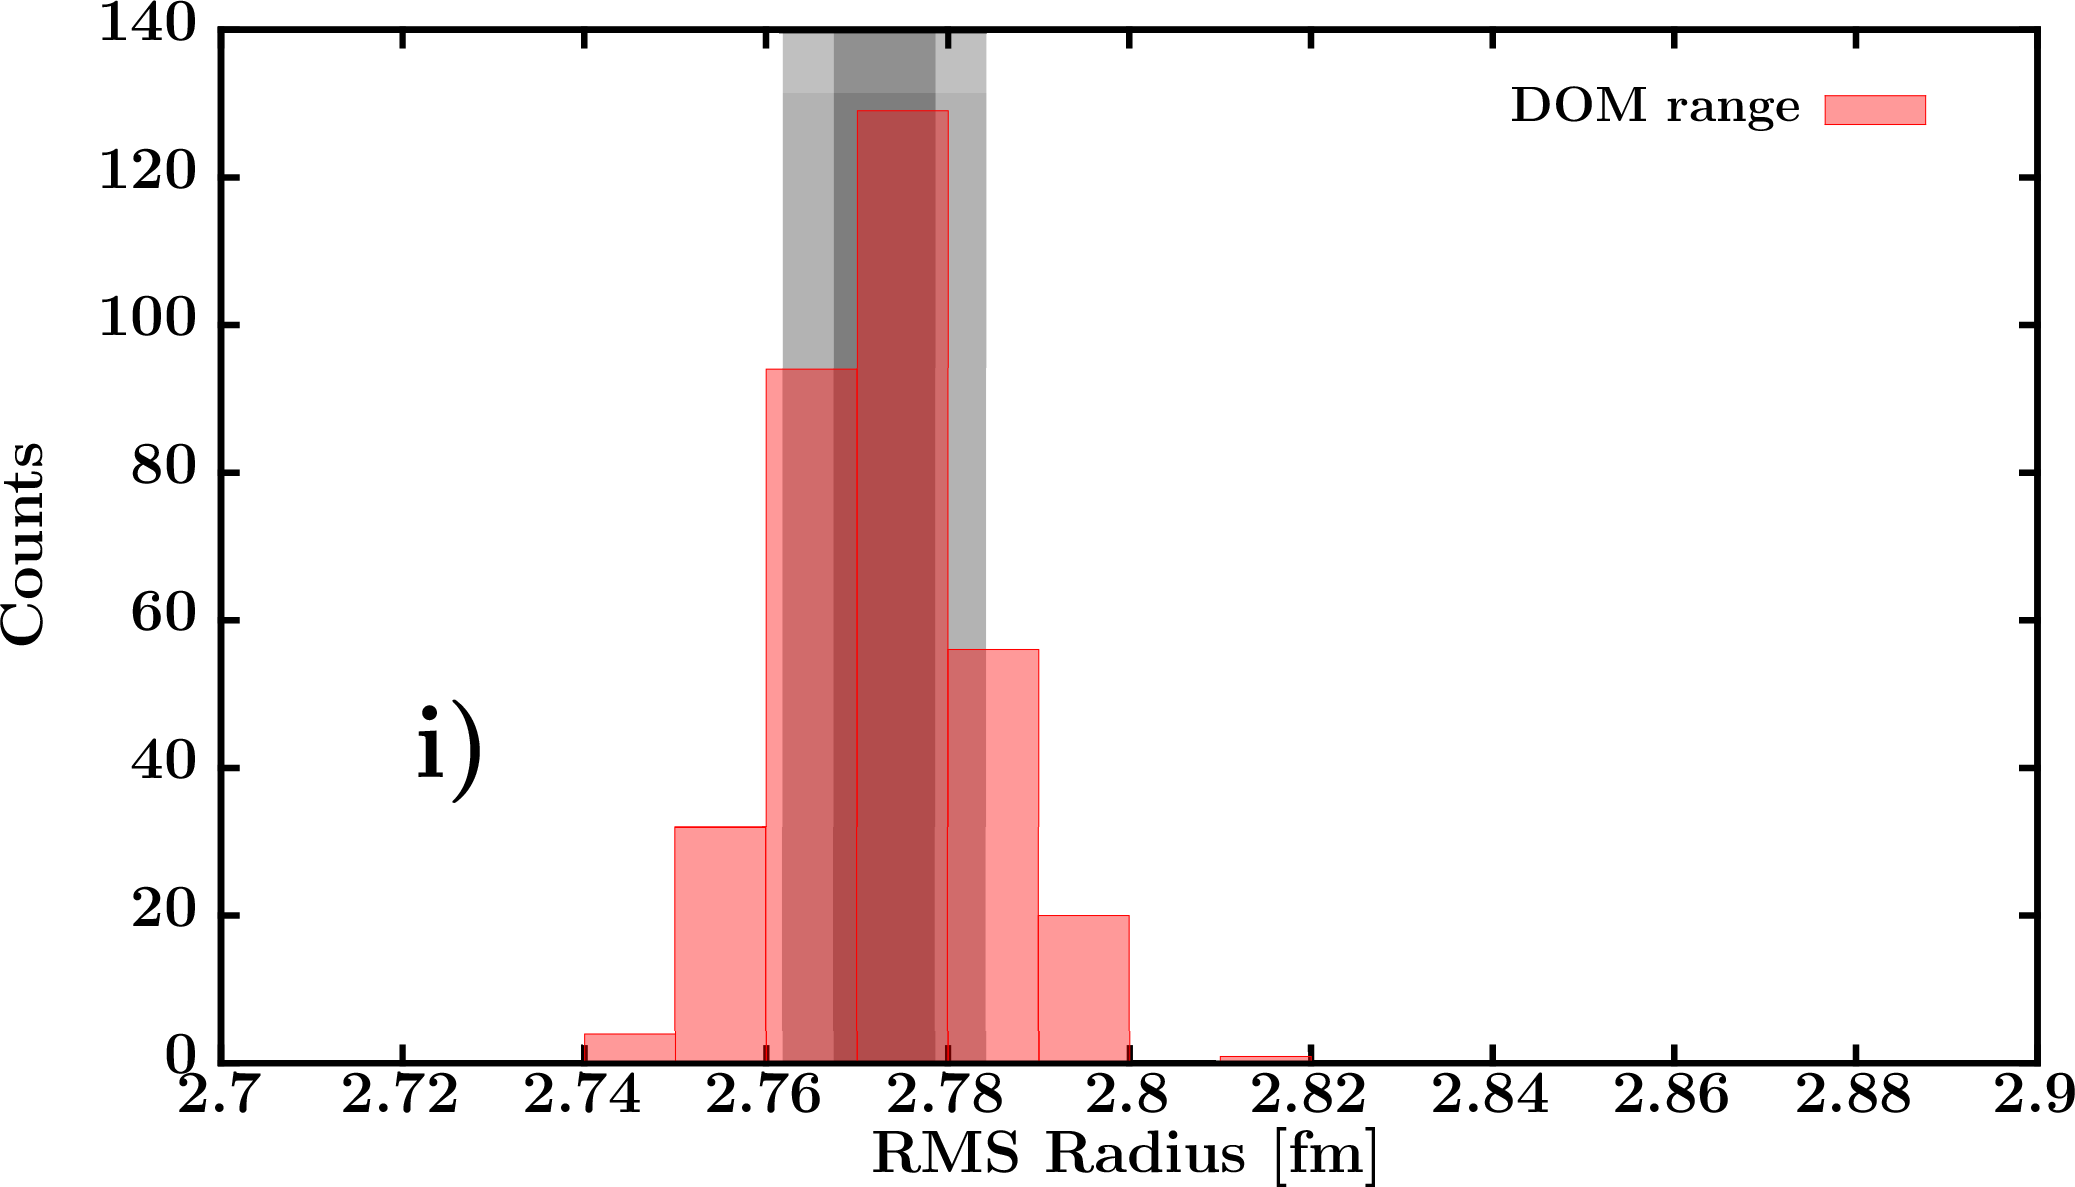
\includegraphics[width=\textwidth]{figures/o18_RMSRadius.png}
        \label{DOM_o18_RMSRadius}
    \end{minipage}
    \begin{minipage}{0.45\textwidth}
        \centering
        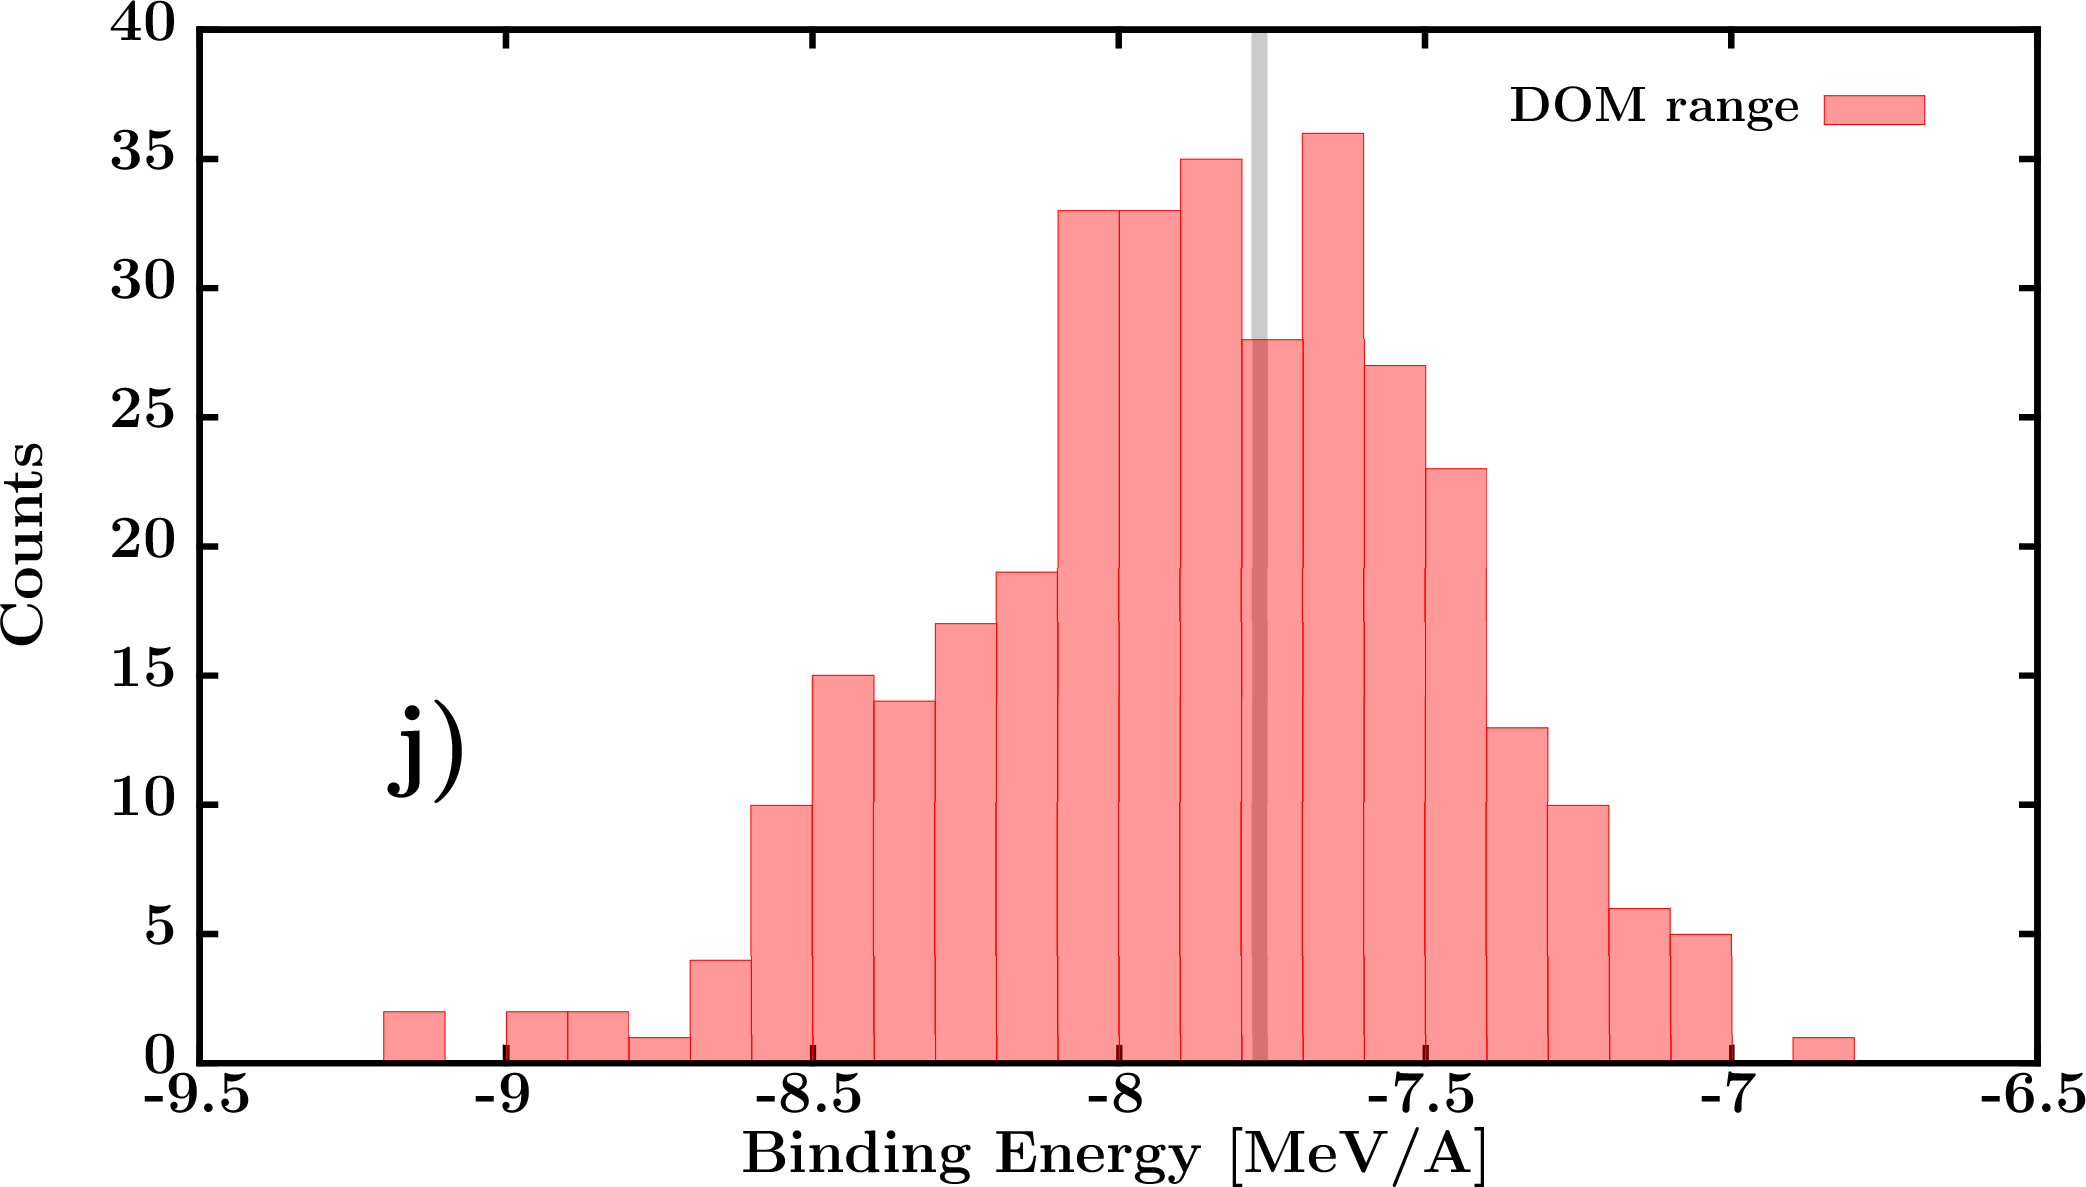
\includegraphics[width=\textwidth]{figures/o18_BE.png}
        \label{DOM_o18_BE}
    \end{minipage}
    \caption{\oEight\ structural data used in DOM fit. Panel a shows the charge
        density distribution: the ``experimental'' data shown here were generated
        by rescaling the \oSix\ distribution (see text). The DOM calculation is
        shown with associated 1$\sigma$ and 2$\sigma$ uncertainty bands.
        Panel b shows the DOM-calculated single-particle energies for protons
        and neutrons with a 1$\sigma$ error band (left side of each subpanel) and
        the known neutron and proton valence level energies, from \cite{AME2016}.
        Panels c and d show the DOM-calculated RMS charge radius and binding energy per
    nucleon, respectively; experimental values/uncertainties are shown in gray.}
    \label{DOM_o18_structural}
\end{figure*}

\textcolor{red}{comments on o18 fit and missing experimental neutron data}

\subsection{Summary fit results for \niEightFour\ and \snTwelveFour\ isotopes}
\textcolor{red}{insert details}

\subsection{Discussion of fit results}
\textcolor{red}{
- Charge density distribution and neutron \tot\ are two most useful data sets
- Lack of elastic neutron scattering data is a big problem for \oEight, \niFour,
and \snTwelveFour.
- \oEight\ missing proton reaction cross section data that appear to be
extremely valuable for fixing the magnitude of the imaginary strength asymmetry
dependence and in turn the neutron skin thickness and extracted valence proton
spectroscopic factors.
}

\section{Conclusion}
By adopting a digitizer-driven
approach, we measured \tot\ on the important closed-shell nuclides
$^{16,18}$O, $^{58,64}$Ni, and $^{112,124}$Sn across more than two orders of
magnitude in energy (3-450 MeV). Except at the highest energies, our results
on natural targets in are good agreement with previous analog-mediated measurements
that required 10-20 times more target material. 

Using these new data and a suite of scattering and bound-state literature data
on \oSixEight, \niEightFour, and \snTwelveFour,
we extracted DOM potentials capable of reproducing a wide range of scattering
and structural data for both neutrons and protons, validating the use of the
DOM away from doubly-closed shells and in systems as light as \oSixEight.
These analyses indicate that isotopically-resolved neutron \tot,
proton \rxn, and charge density distribution data are valuable assets for
constraining optical potentials, especially the imaginary and
asymmetry-dependent components.

%Our results are in good agreement with spectroscopic information
%from (e,e'p) measurements and show the sensitivity of nucleon matter density
%distributions to SRCs, which push nucleon density outward from the core and
%to higher angular momenta.

\section{Acknowledgements}
\textcolor{red}{insert acknowledgements}

\bibliography{references}
\begin{thebibliography}{32} \expandafter\ifx\csname
        natexlab\endcsname\relax\def\natexlab#1{#1}\fi \expandafter\ifx\csname
        bibnamefont\endcsname\relax \def\bibnamefont#1{#1}\fi
        \expandafter\ifx\csname bibfnamefont\endcsname\relax
        \def\bibfnamefont#1{#1}\fi \expandafter\ifx\csname
        citenamefont\endcsname\relax \def\citenamefont#1{#1}\fi
        \expandafter\ifx\csname url\endcsname\relax \def\url#1{\texttt{#1}}\fi
        \expandafter\ifx\csname urlprefix\endcsname\relax\def\urlprefix{URL
        }\fi \providecommand{\bibinfo}[2]{#2}
        \providecommand{\eprint}[2][]{\url{#2}}

\end{thebibliography}

\end{document}
